	\documentclass[8pt]{beamer}
\usepackage[utf8]{inputenc}

\usetheme{Madrid}

%% ADDITIONAL NICOLÁS
\usepackage{ragged2e}
\usepackage{amssymb}
\usepackage{subcaption}

\usefonttheme{serif}
\definecolor{UBCblue}{rgb}{0.01569, 0.11765, 0.25882} % PSU Blue
\usecolortheme[named=UBCblue]{structure}

%% ADDITIONAL NICOLÁS


\newcommand{\locx}{\mathbf{x}}
\newcommand{\vele}{\mathbf{e}_\alpha}
\newcommand{\kronecker}{\delta_{\alpha \beta}}
%------------------------------------------------------------
%This block of code defines the information to appear in the
%Title page
\title[Weekly Reports] %optional
{PhD in Energy and Mineral Engineering at PSU}

\subtitle{Nicolás's Research - Reports}

\author[Nicolás Bueno] % (optional)
{Nicolás Bueno\inst{1} \and Advisor: Dr. Ayala\inst{1} \and Co-advisor: Dr. Mehmani\inst{1}}

\institute[EME] % (optional)
{
	\inst{1}%
	Department of Energy and Mineral Engineering\\
	Penn State University\\
	
\includegraphics[height=1cm]{pics/PSU_EMS.png}
}

\date[Spring 2022] % (optional)
{}

%\logo{
\includegraphics[height=1cm]{pics/PSU_EMS.png}}

%End of title page configuration block
%------------------------------------------------------------



%------------------------------------------------------------
%The next block of commands puts the table of contents at the 
%beginning of each section and highlights the current section:

\AtBeginSection[]
{
	\begin{frame}
		\frametitle{Table of Contents}
		\tableofcontents[currentsection]
	\end{frame}
}
%------------------------------------------------------------


\begin{document}
	
	%The next statement creates the title page.
	\frame{\titlepage}
	
	%---------------------------------------------------------
	%This block of code is for the table of contents after
	%the title page
	\begin{frame}
		\frametitle{Table of Contents}
		\tableofcontents
	\end{frame}
	%---------------------------------------------------------
	
	\justifying
	\section{Spring 2022}
	
	\subsection{Report Jan 24 - 2022}
	\label{}
	\justifying
	\begin{frame}
		\textbf{Report Jan 24 - 2022}\\~\\
		Main discussion points:
		\begin{itemize}
			\item Cheng's paper
			\item LBM Code state
			\item Short-term Medium-term objectives
		\end{itemize}
	\end{frame}
	
	\begin{frame}{Cheng's paper}
		Bulk equation for the Shan-Chen force:
		\begin{equation*}
		\mathbf{F} = -G \psi(x) \sum_i \omega_i \psi(x+\mathbf{c}_i \delta t) \mathbf{c}_i \, \, \, \, \, \psi := \sqrt{\frac{2(P^{\text{\tiny EoS}}-c_s^2\rho)}{G \delta t c_s^2}}
		\end{equation*}
		\begin{itemize}
			\item MRT model
			\item Multi-component partially miscible
		\end{itemize}
	\end{frame}
	
	\begin{frame}{LBM state}
		This I advanced before last state:
		\begin{itemize}
			\item Tried the binary printing (unsuccessful)
			\item Run the single component multi-phase model (successful)
			\item Equation to count the number of molecules in a lattice. 
			\item Short-term mid-term objectives
		\end{itemize}
	\end{frame}

	\begin{frame}{van der Waals validation}
		\begin{figure}
			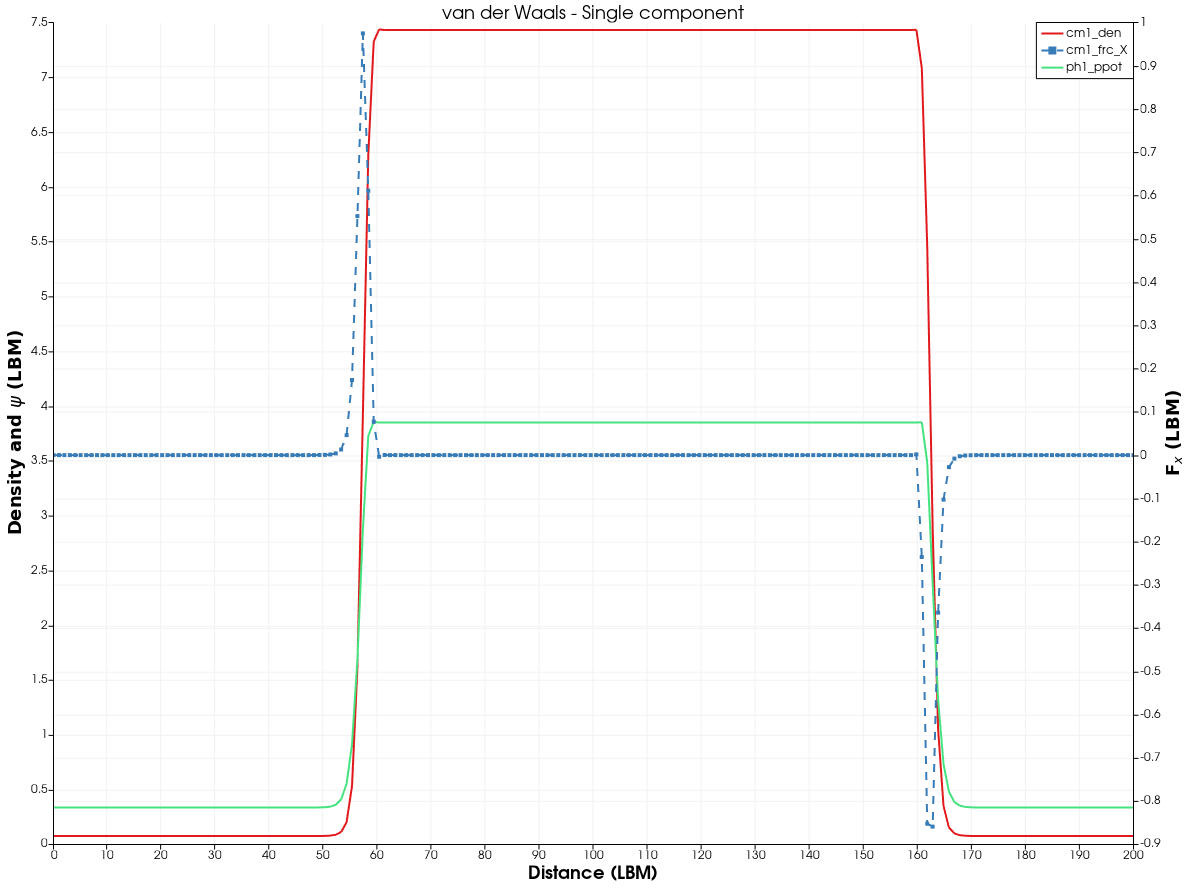
\includegraphics[scale=0.2]{pics/vdwValidation.png}
		\end{figure}
	\end{frame}

	\begin{frame}{Peng Robinson validation}
		\begin{columns}
			\column{0.4\textwidth}
			\begin{figure}
				\centering
				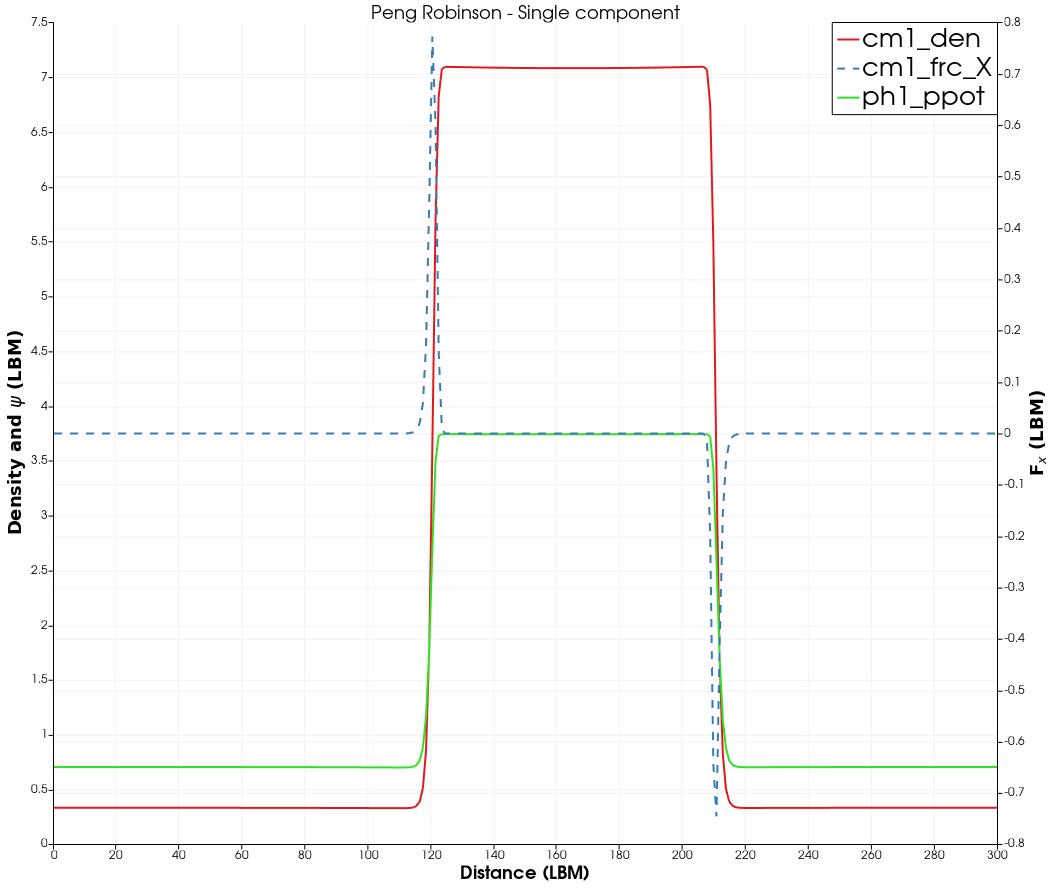
\includegraphics[scale=0.12]{pics/prValidation.png}
				\caption{}   
			\end{figure}
			\column{0.4\textwidth}
			\begin{figure}
				\centering
				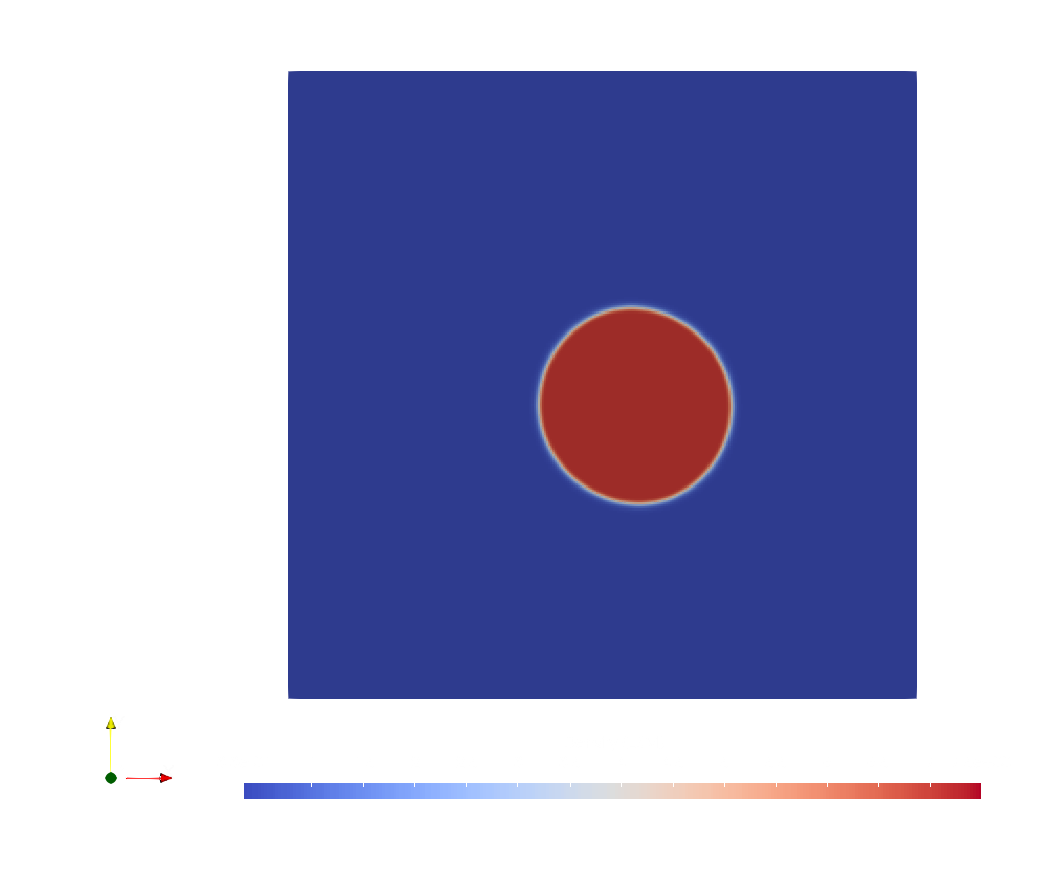
\includegraphics[scale=0.15]{pics/prValidation2.png}
			\end{figure}
		\end{columns}
	\end{frame}

	\begin{frame}{Where I am going?}
		I was rediscovering the concept of $\psi$ that now belongs to the bulk (phase) entity. In Kruger's book is assigned to each component, so each components computes its own SC force. Other forces split according to $\rho_i$.\\
		Two components structure is ready to start building the 2-component case that Cheng uses for validation. 
	\end{frame}
	\begin{frame}{Actions}
		\begin{itemize}
			\item Dry-run of research proposal for qualifying exam.Deep dive into literature looking for problems in current problems and interesting applications (reactions-solute transport-energy-multiphase).
			\item LBM tutorials is the next short-term project
			\item Finish my own code to run the Cheng's cases in our simulator. 
			\item Long-term: evaluate the Kruger's perspective of calculating SC per component.
		\end{itemize}
	\end{frame}
	
	%---------------------------------------------------------
	%---------------------------------------------------------
	\subsection{Report Jan 31 - 2022}
	\label{}
	\justifying
	\begin{frame}
		\textbf{Report Jan 31 - 2022}\\~\\
		\begin{itemize}
			\item Code and Cheng's paper
			\item SPH for EME 521
			\item Time demand
			\item Others
			\begin{itemize}
				\item Dr. Mehmani meetings (I'll start slow). 
				\item Summer 2022
				\item Almost null offer research-related. Italian courses.
				\item STAP (Summer Tuition Assistance Program)
				\item Penn State Vita (Taxes)
				\item 2022 Fuel Science Graduate Awards
				\item Own website
			\end{itemize}
			\item Lost.
		\end{itemize}
	\end{frame}
	
	\begin{frame}{Code}
		Multiphase validations: van der Waals (flat interface, droplet), Peng-Robinson (making use of velocity redefinition and $\beta$ parameter).\\
		Cheng redefined the velocity for the Guo's scheme as:
		
		\begin{equation}
			\mathbf{u}^{mod} = \mathbf{u} + \frac{\beta \mathbf{F}}{(\tau - 0.5)\psi^2}
		\end{equation}
		
		The other velocity definitions remain. Without this term, the PR case diverges. Also $G$ affects stability.
		
	\end{frame}
	
	\begin{frame}{Code - Peng Robinson validation}
		\begin{columns}
			\column{0.4\textwidth}
			\begin{figure}
				\centering
				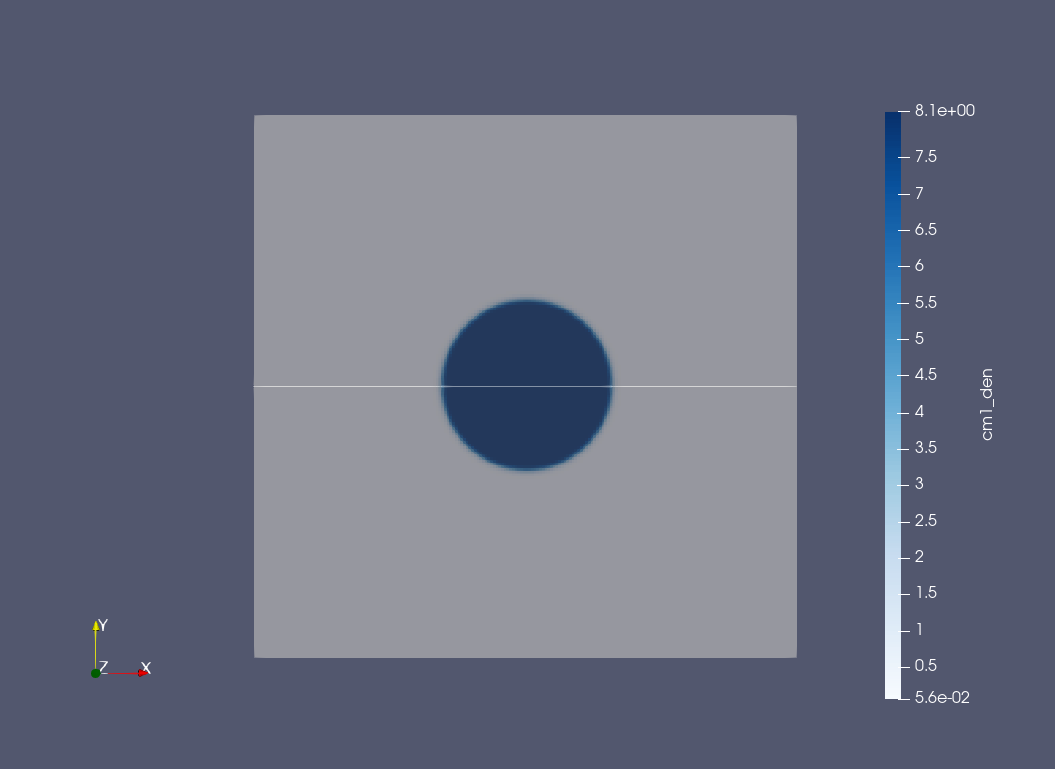
\includegraphics[scale=0.12]{pics/prDroplet1C.png}
				\caption{}   
			\end{figure}
			\column{0.4\textwidth}
			\begin{figure}
				\centering
				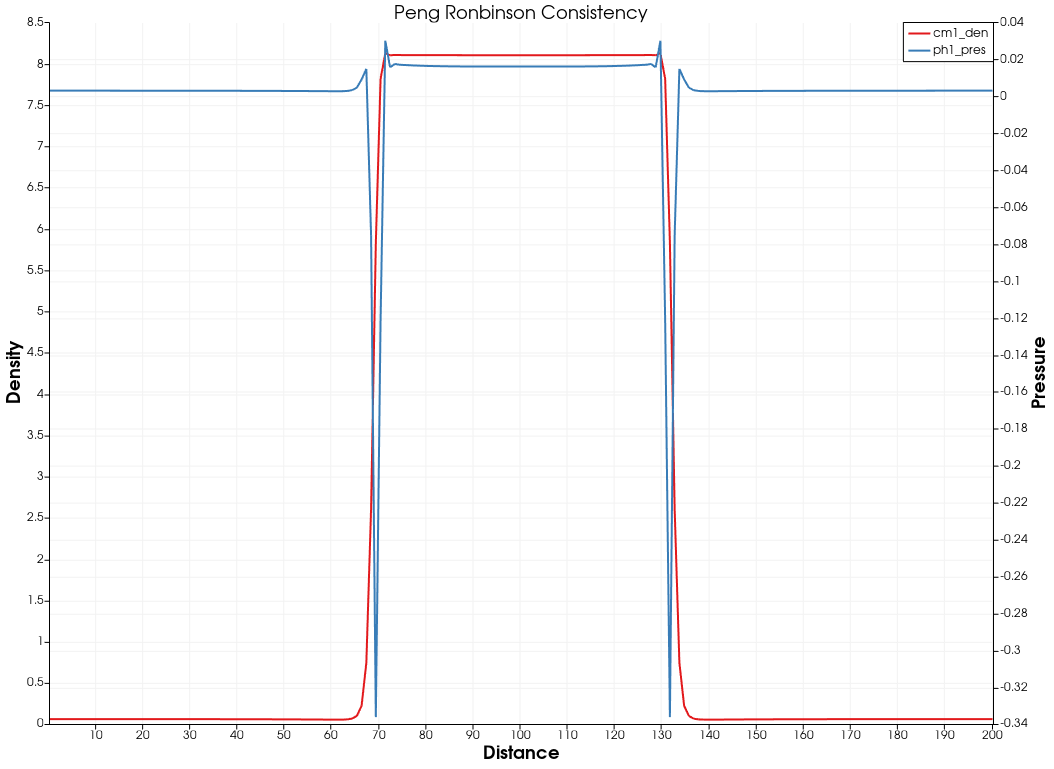
\includegraphics[scale=0.15]{pics/prDroplet1C_2.png}
			\end{figure}
		\end{columns}
	\end{frame}
	
	\begin{frame}{Code - New features}
		\begin{itemize}
			\item Now we can have $N_F$ forces of different nature. All are grouped and discretized in the velocity space together.
			\item We have now a new force to compute $\psi^i$ and thus calculate a force per component.
			\item Each component relaxes with its own $\tau^i$, allowing different viscosities.
			\item Reading density/pressure fields for every component, and a common velocity field.
		\end{itemize}
		Current problems:
		\begin{itemize}
			\item Force only working for periodic BC.
			\item Still not implemented the force fluid/solid
			\item Instability (due to BGK)
		\end{itemize}
		 
	\end{frame}
	
	\begin{frame}{Code}
		\begin{itemize}
		\item Can the pressure of the gas be higher than the liquid? What if we initialize a bubble instead of a droplet?
		\item Validate Young-Laplace?
		\item I am now setting a 2C 2P problem to validate the code. I can try both, immiscible and miscible, as both implementations are there and the only change is the $\psi$ definition.
		\item Injecting A into a system full of B. How does it look like?
		\item What 1C complex systems can we simulate? Water hammer effect?
		\end{itemize}
		Ready for meeting with Pr. Orlando for program. language discussions, questions about implementations, and possible feedback (I need the time to compile the material).\\~\\
		
		PBM: RR procedure. I'll program the minimization algorithm, but try to implement Eigen, a library to solve $\mathbf{A \cdot x} = \mathbf{b}$.
	\end{frame}
	
	\begin{frame}{Research}
		I definitely want to use my research for applying the LBM to a particular field. In contrast, my Master's Thesis was only computational, with validations, but did not include any experimental/real data of any type. Questions I have:
		\begin{itemize}
			\item Bubbles, coalescence, and their viscosity effect
			\item CO$_2$ plume generation.
			\item Interaction between fluids and rock (swelling, mineralization, adsorption)
			\item Rock deformation? Does imply FEM? Too complicated? 
			\item Questions about $\sigma$ in 3-P systems. I don't know? Nobody knows? Film drainage. Oil spills. Receding / advancing $\theta$ 
			\item Can we derive a $k_r$ label-blind with hysteresis, based on 3P simulations?
		\end{itemize}
		
	\end{frame}

	\begin{frame}{Actions}
		\begin{itemize}
			\item Yes, start learning SPH. 
			\item Look for internships in companies and research labs in the US. In Summer, if nothing appears, we will focus on research. Do not lose contacts and willingness to participate in new things.
			\item Apply to Fuel Award and Nico SPE Awards
			\item Go for MRT. Write equations. Pr. Orlando presentation. Think in 2C cases that validates our understanding. 2 non interacting components (miscible). Then partially miscible. 
			\item Bubbles as an interesting topic to work with in LBM. There may be other options.
		\end{itemize}
	\end{frame}
	%---------------------------------------------------------
	%---------------------------------------------------------
	
	\begin{frame}{Discussion}
		Discussion...
	\end{frame}
	
	%---------------------------------------------------------
	%---------------------------------------------------------
	
	\subsection{Report Feb 7 - 2022}
	\label{}
	\justifying
	\begin{frame}
		\textbf{Report Feb 7 - 2022}\\~\\
		\begin{itemize}
			\item Cheng's coding error in modified velocity.
			\item MRT implementation. Facts and difficulties:
			\begin{itemize}
				\item Vectorized implementation. Still have problems with $\mathbf{m}^{\text{eq}}$. Works only in manual computing.
				\item More validation cases. I only picked one.
				\item Recent result: yesterday.
			\end{itemize}
			\item Peng Robinson inconsistency: I have to revisit the PR results with BGK. I thing it may be converging to densities slightly away from equilibrium.
			\item Dr. Mehmani suggestions.
			
		\end{itemize}
	\end{frame}
	

	\begin{frame}{MRT Validation}
		\begin{figure}
			\centering
			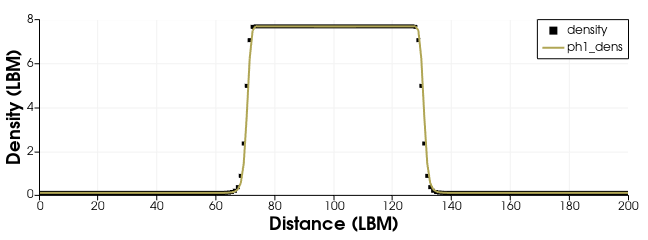
\includegraphics[scale=0.4]{pics/MRTValDen.png}
		\end{figure}
		\begin{figure}
			\centering
			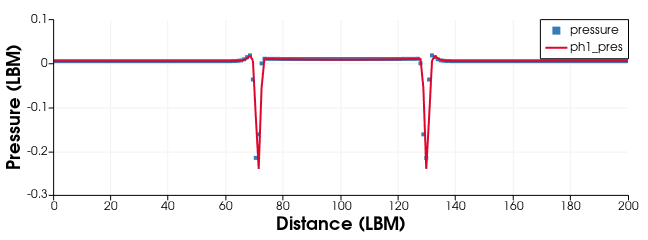
\includegraphics[scale=0.4]{pics/MRTValPres.png}
		\end{figure}
	
	\end{frame}
	\begin{frame}{Actions}
		\begin{itemize}
			\item Prepare meeting with Cheng: velocity modification, and MRT parameters. Source of validation.
			\item Trace a path for validation: Oscillating droplet, tube oscillation. 
			\item Reading CO$_2$ with oil trapping and water different mechanisms and modeling.
			\item Share code.
			
		\end{itemize}
	\end{frame}
	
	
	%---------------------------------------------------------
	%---------------------------------------------------------
	
	\subsection{Report Feb 14 - 2022}
	\label{}
	\justifying
	\begin{frame}
		\textbf{Report Feb 14 - 2022}\\~\\
		\begin{itemize}
			
			\item BGK and MRT validations
			\begin{itemize}
				\item Several cases tested: see the LBM private document
				\item How to set fluid viscosity with MRT?
				\item I had to change Cheng's diffuse width.
			\end{itemize}
			
			\item Dr. Mehmani suggestions.
			\item Questions
			\begin{itemize}
				\item Point-distributed parameter and point-centered (?) parameter
				\item Fluid in tension LBM?
				\item Motivation. Self-propulsion, drop collision, microemulsions: \href{https://www.youtube.com/watch?v=arpGntfrg4s}{link to Youtube}
			\end{itemize}
			
		\end{itemize}
	\end{frame}

	\begin{frame}{BGK Validation - Cheng's code}
		\begin{figure}
			\centering
			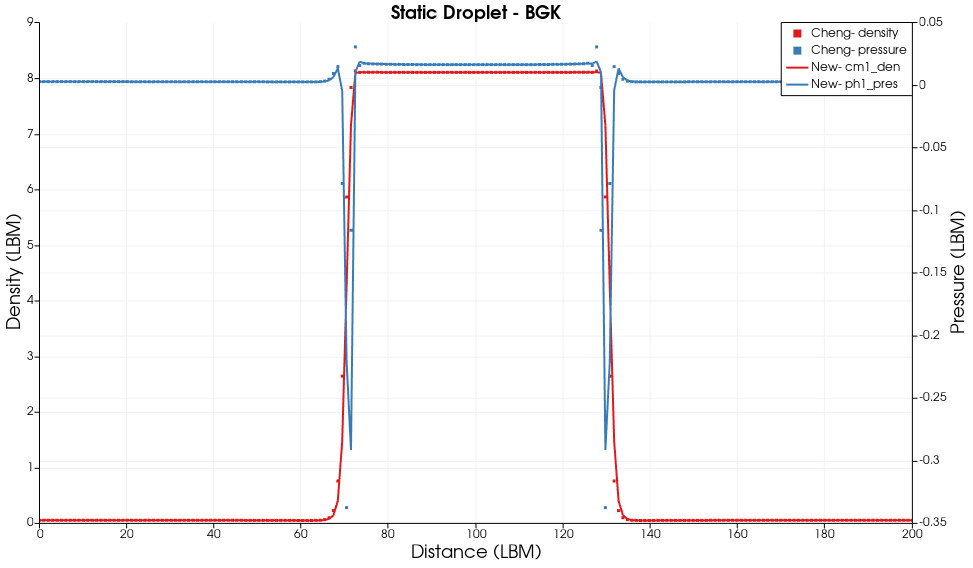
\includegraphics[scale=0.3]{pics/BGK_StaticDroplet.png}
		\end{figure}
	\end{frame}
	\begin{frame}{BGK Validation - Cheng's code}
		\begin{figure}
			\centering
			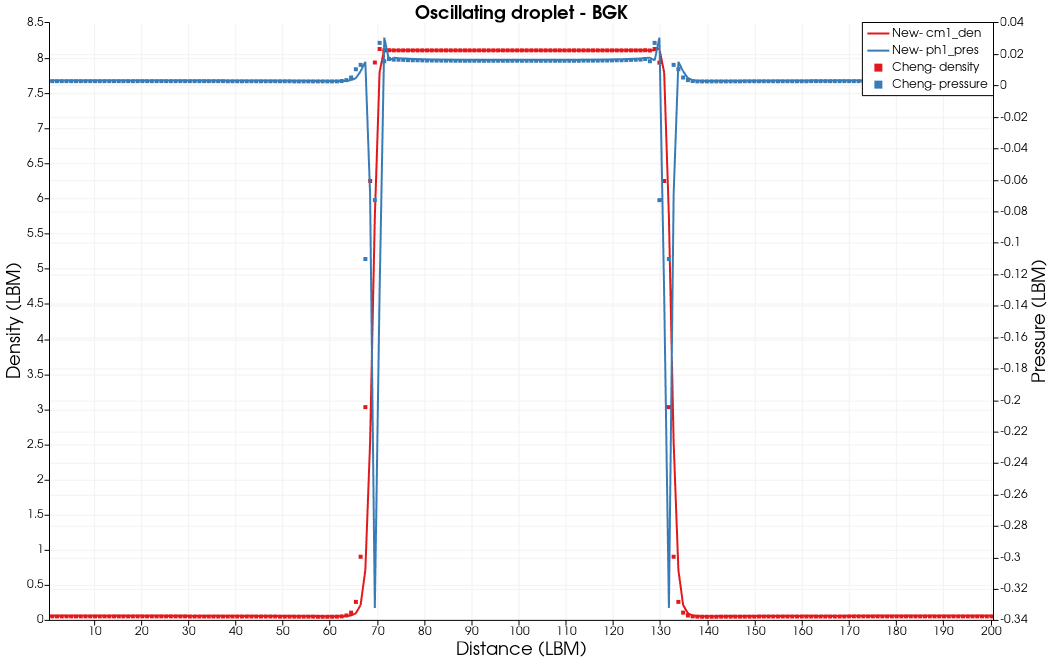
\includegraphics[scale=0.3]{pics/BGK_OscDroplet_PRHO.png}
		\end{figure}
	\end{frame}
	\begin{frame}{BGK Validation - Cheng's code}
		\begin{figure}
			\centering
			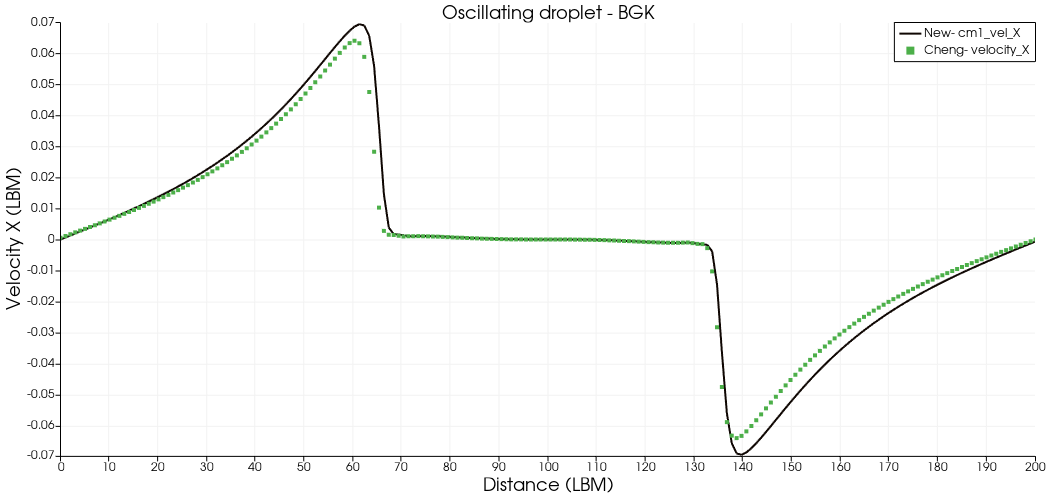
\includegraphics[scale=0.3]{pics/BGK_OscDroplet_VelProf.png}
		\end{figure}
	\end{frame}
	\begin{frame}{BGK Validation - Cheng's code}
		\begin{figure}
			\centering
			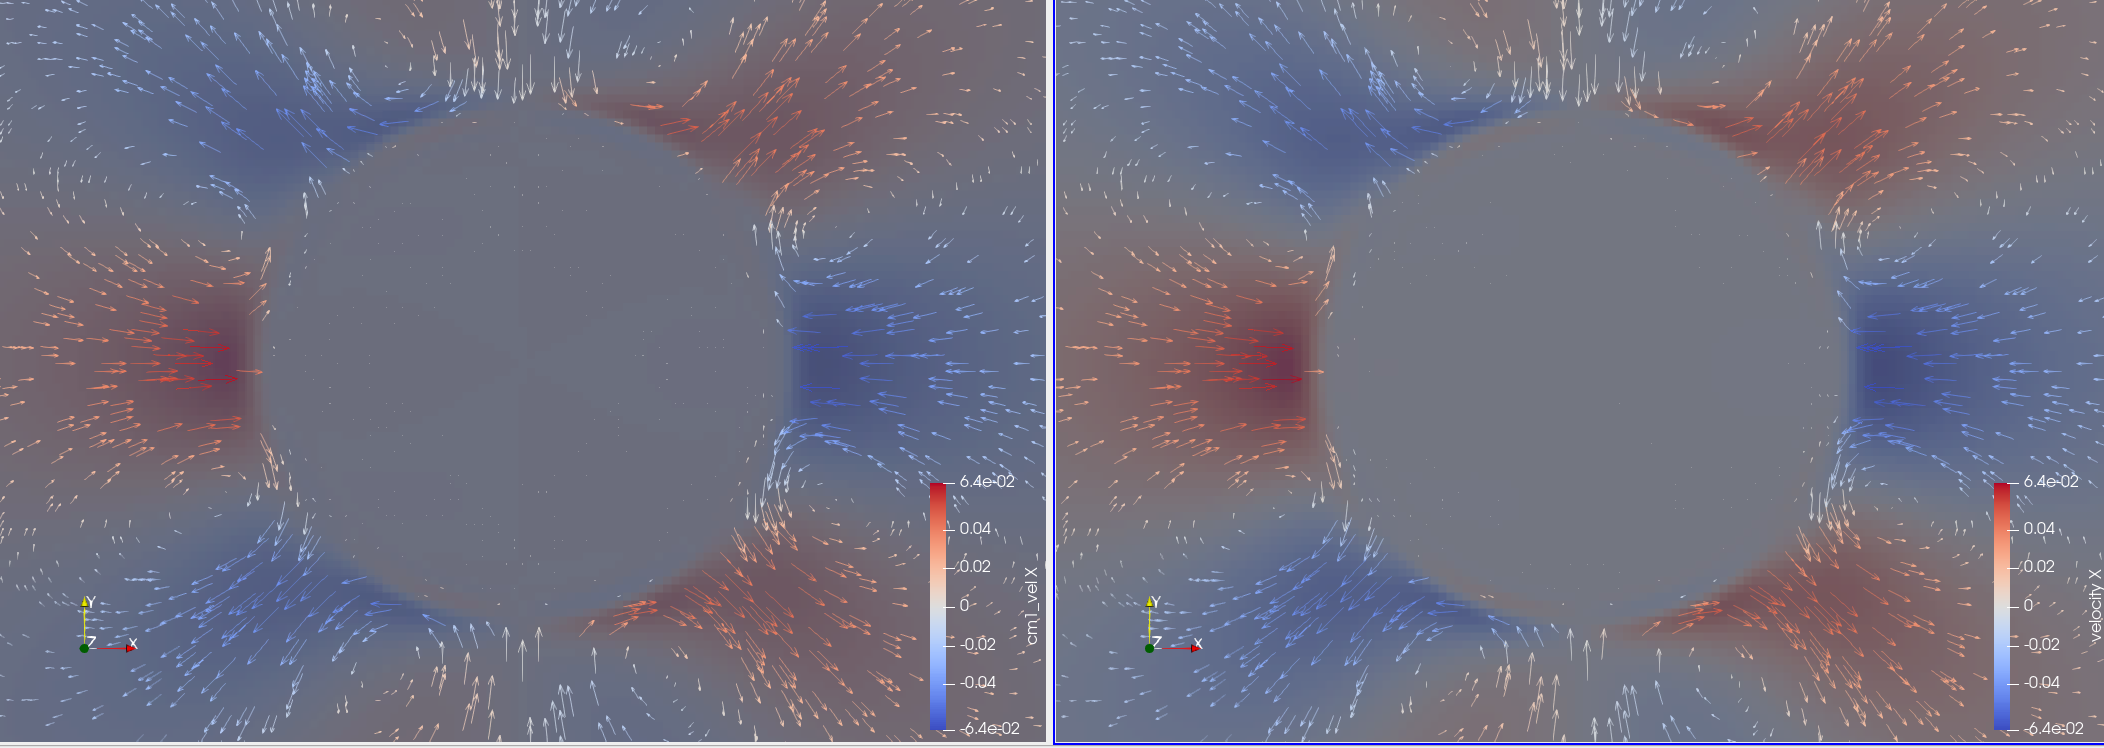
\includegraphics[scale=0.14]{pics/BGK_VelFieldComparison.png}
		\end{figure}
	\end{frame}
	\begin{frame}{BGK Validation - Cheng's code}
		\begin{figure}
			\centering
			\includegraphics[scale=0.14]{pics/OScDroplet_BGK_Axis.png}
		\end{figure}
	\end{frame}
	
	
	\begin{frame}{MRT Validation - Cheng's code}
		\begin{figure}
			\centering
			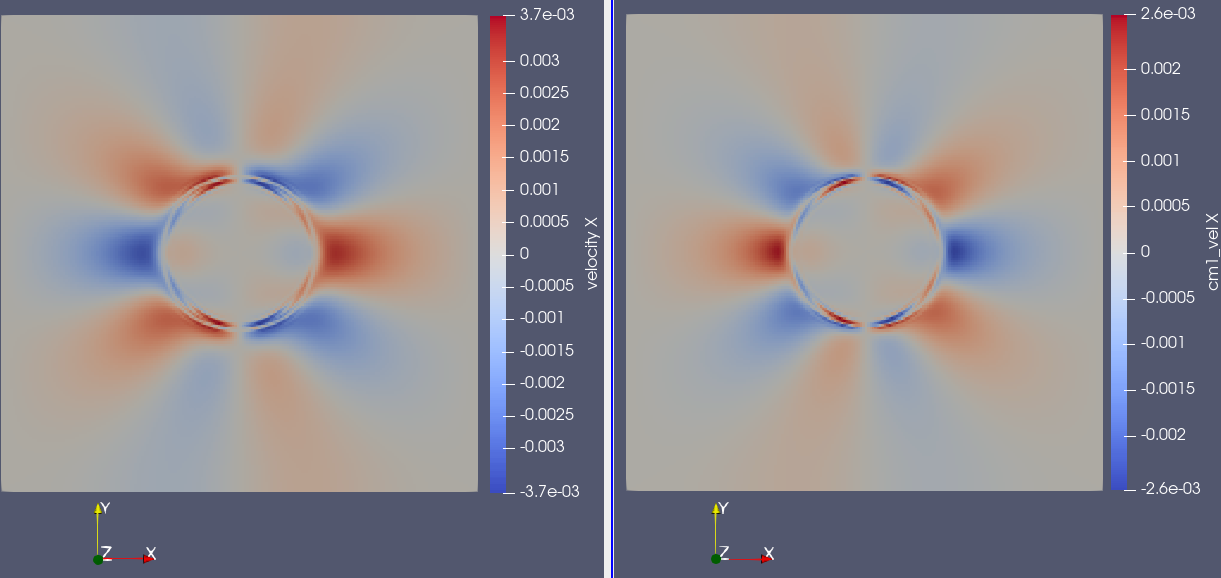
\includegraphics[scale=0.25]{pics/MRT_StaticDroplet_VelField.png}
		\end{figure}
	\end{frame}
	\begin{frame}{MRT Validation - Cheng's code}
		Attached video.
		\begin{figure}
			\centering
			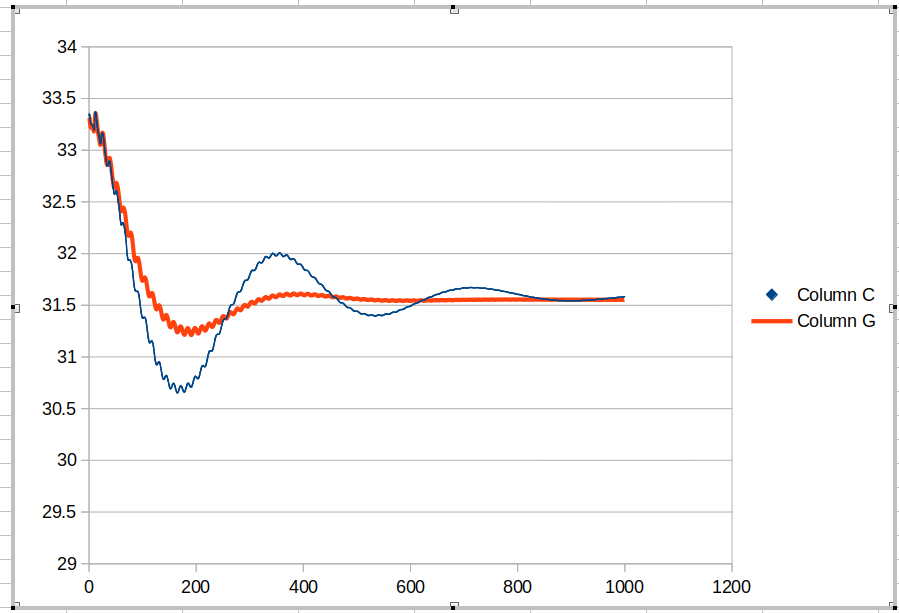
\includegraphics[scale=0.25]{pics/MRT_oscillatingAxis.png}
		\end{figure}
	\end{frame}
	
	\begin{frame}{For analytical solutions}
		\begin{itemize}
			\item How to convert a single component droplet surrounded by its vapor, to a droplet surrounded by empty space? Is the frequency of the oscillation the same in both cases.
			
			\item Analytical solutions and reported cases:
			\begin{itemize}
				\item Oscillating droplet
				\item Rising bubble (very interesting!)
				\item Square drop as IC
				\item Rayleigh-Taylor instability (heavy fluid supported against gravity)
				\item Induced translation by Marangoni-effect (variable $\sigma$ field)
				\item Bubble break-up due to variable $\sigma field$
			\end{itemize}
		\end{itemize}
	\end{frame}

	\begin{frame}{Actions}
		\begin{itemize}
			\item Keep preparing Cheng's meeting
			\item Go back to BGK and compare oscillations
			\item Find differences with MRT for oscillating droplet
			\item Start reading LAMP reference and Cheng's reports to compare against analytical solution
			\item Go for the 2 components case
		\end{itemize}
	\end{frame}
	
	
	%---------------------------------------------------------
	%---------------------------------------------------------
	
	
	\subsection{Report Feb 21 - 2022}
	\label{}
	\justifying
	\begin{frame}
		\textbf{Report Feb 21 - 2022}\\~\\
		\begin{itemize}
			\item BGK and MRT validations
			\item Viscosity per phase-per component
			\item Rising droplet (video)
			\item Marangoni flow (papers based on Phase-Field and Free energy)
			\item Questions
			\begin{itemize}
				\item Point-distributed parameter and point-centered (?) parameter
				\item Fluid in tension LBM?
				\item Motivation. Self-propulsion, drop collision, microemulsions: \href{https://www.youtube.com/watch?v=arpGntfrg4s}{link to Youtube}
			\end{itemize}
			\item What to present in next meeting?
		\end{itemize}
	\end{frame}

	\begin{frame}{Oscillating droplet}
		\begin{figure}[h]
			\centering
			\begin{subfigure}{.5\textwidth}
				\centering
				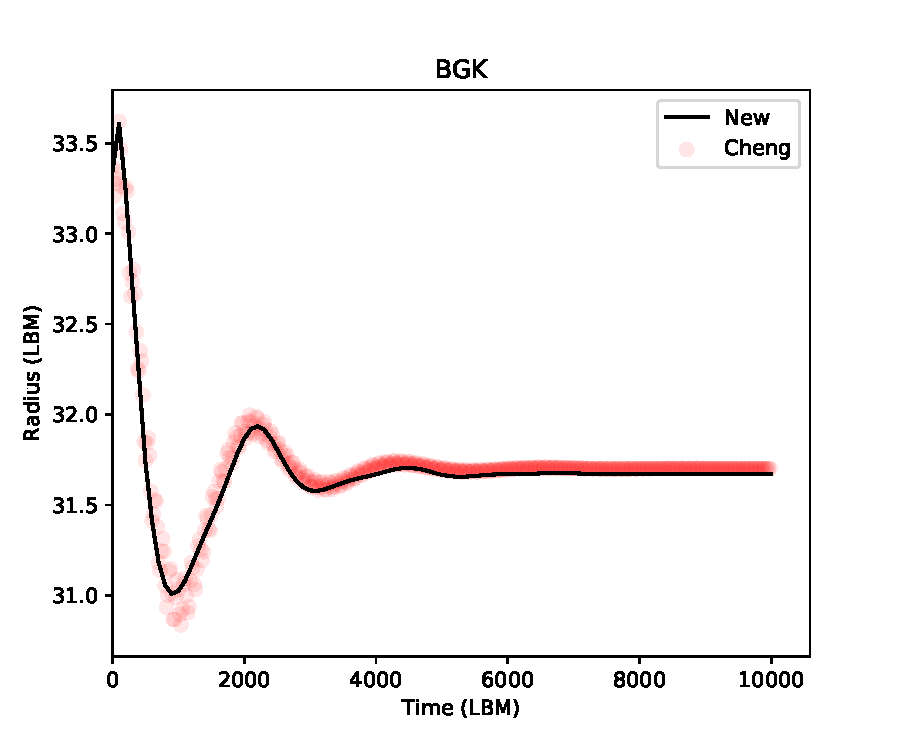
\includegraphics[width=.9\linewidth]{pics/BGKOsc.pdf}
				\caption{BGK}
				\label{fig:sub1}
			\end{subfigure}%
			\begin{subfigure}{.5\textwidth}
				\centering
				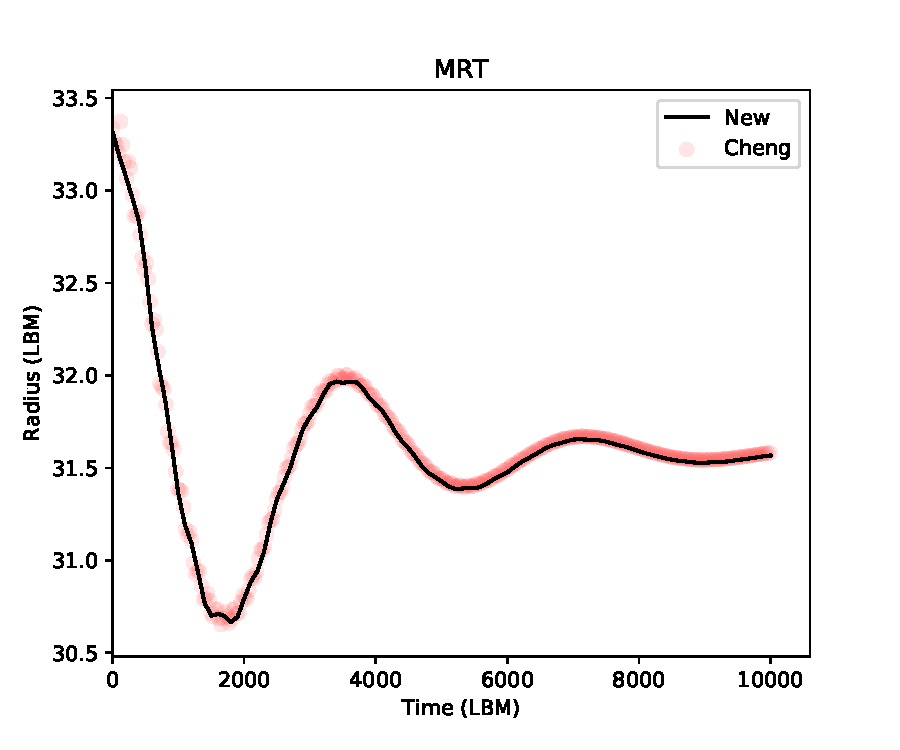
\includegraphics[width=.9\linewidth]{pics/MRTOsc.pdf}
				\caption{MRT}
				\label{fig:sub2}
			\end{subfigure}
			\caption{Oscillation droplet case. Viscosities are different in each case.}
			\label{fig:osci}
		\end{figure}
	\end{frame}

	\begin{frame}{Thursday meeting}
		\begin{itemize}
			\item Motivation of new code
			\item Current validations
			\item Current status
			\item Questions about: boundary conditions, global density increase, dynamic validations:
			\begin{itemize}
				\item Oscillating droplet (ready). For which conditions, an analytical solution exists? Droplet in void space?
				\item Rayleigh-Taylor instability (oscillating capillary tube)
				\item Rotating droplet (any analytical solution)
			\end{itemize}
		\end{itemize}
	\end{frame}
	
	
	
	\begin{frame}{Actions}

	\end{frame}

	%---------------------------------------------------------
	%---------------------------------------------------------

	\subsection{Weekly meeting - LBM - Feb 24 - 2022}
	\label{}
	\justifying
	\begin{frame}{Weekly meeting - LBM}
		\textbf{Feb 24 - 2022}\\~\\
		\begin{itemize}
			\item LBM Code - New version (motivation, state, and validation)
			
			\item Questions about the LBM formulation
		
			\item Paper (Dynamic validations)
		\end{itemize}
	\end{frame}
	
	\begin{frame}{LBM Code}
		
		Motivation: 
		\begin{itemize}
			\item 3D version for arbitrary domains, forces, and boundary conditions
			\item Future parallelization
			\item Coupling with other transport equations
		\end{itemize}
	
		~\\\textbf{General description}: Fortran 90, Object Oriented, LBM code for multi-component ($N_c$) mixtures. Output in VTK format. Main classes:
		\begin{itemize}
			\item Components - Phase - Mixture - Equation of state
			\item LBM Functions (Parameters - Coll. Operators) 
			\item Domain - Global Properties
			\item Forces - Boundaries
		\end{itemize}
		Desired simulation setup is given through input files (parameters, domain, initial conditions).
	\end{frame}
	
	\begin{frame}{Validations}
		
		The main validation sources are: analytical solutions, Cheng's codes, qualitative physics understanding.\\~\\

		
		\begin{columns}[T]
			
			\column{0.5\textwidth}
			Single phase:
			\begin{itemize}
				\item Channel flow ($\mathbf{F}$ \& $\nabla p$-driven)
				\item Couette flow (plates)
				\item Cylinder (turbulent)
				\item Cavity flow
				\item Porous medium
			\end{itemize}
			
			\column{0.5\textwidth}
			Multiphase:
			\begin{itemize}
				\item Static droplet
				\item Oscillation droplet
				\item Falling droplet
			\end{itemize}
		\end{columns}
	\end{frame}

	\begin{frame}{Single phase validations (quantitative)}
		\begin{figure}[h]
			\centering
			\begin{subfigure}{.5\textwidth}
				\centering
				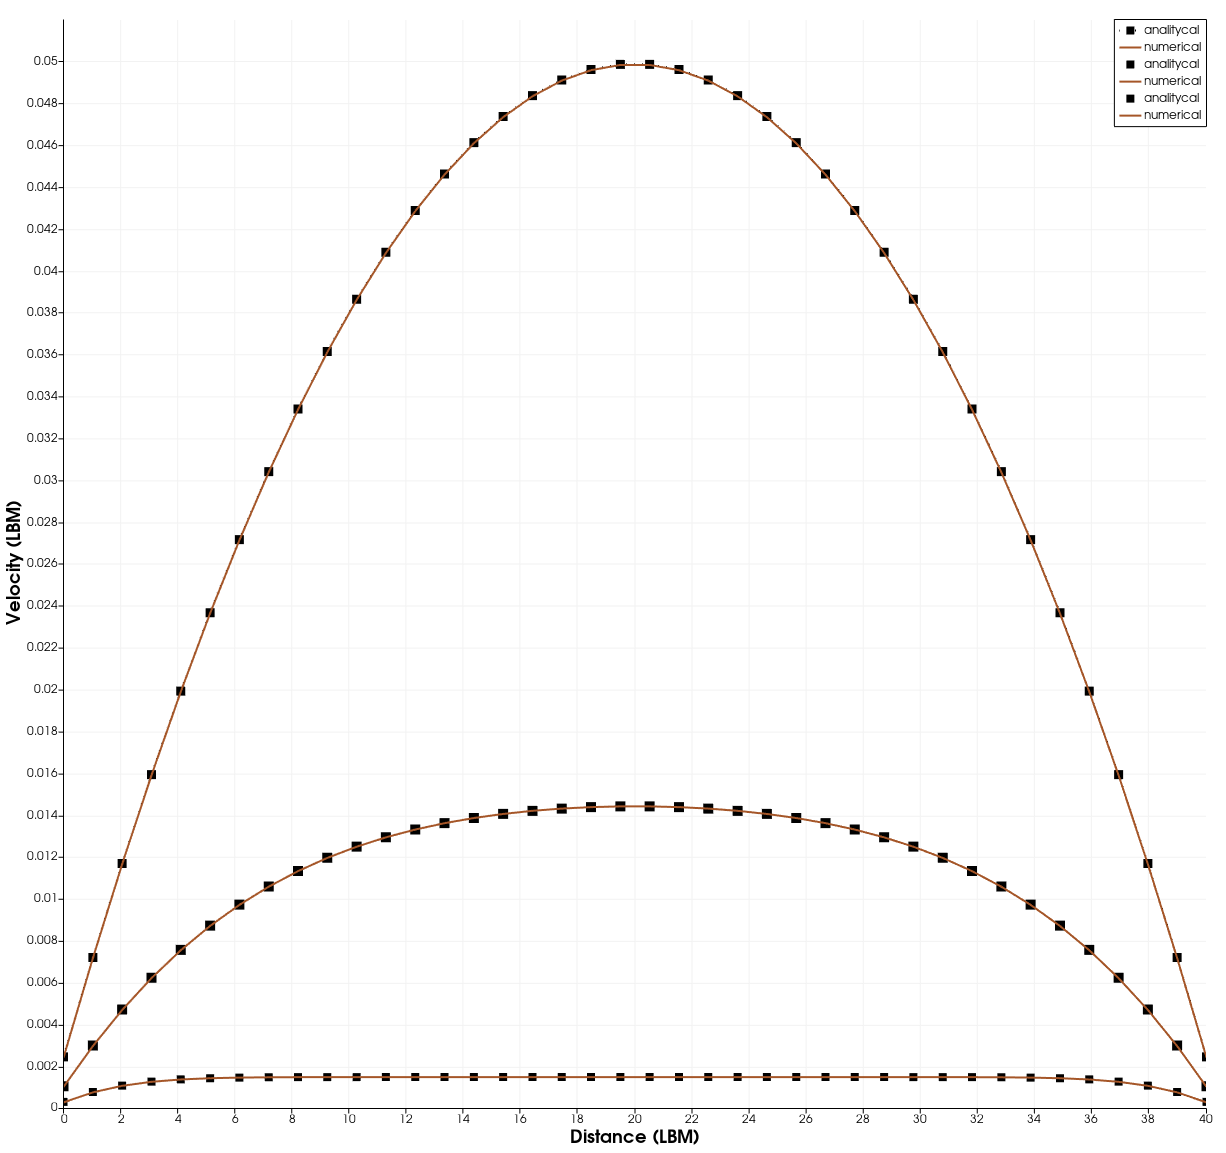
\includegraphics[width=.9\linewidth]{pics/channelForceDrivenValidation.png}
				\caption{$\mathbf{F}$-driven channel flow}
				\label{fig:sub1}
			\end{subfigure}%
			\begin{subfigure}{.5\textwidth}
				\centering
				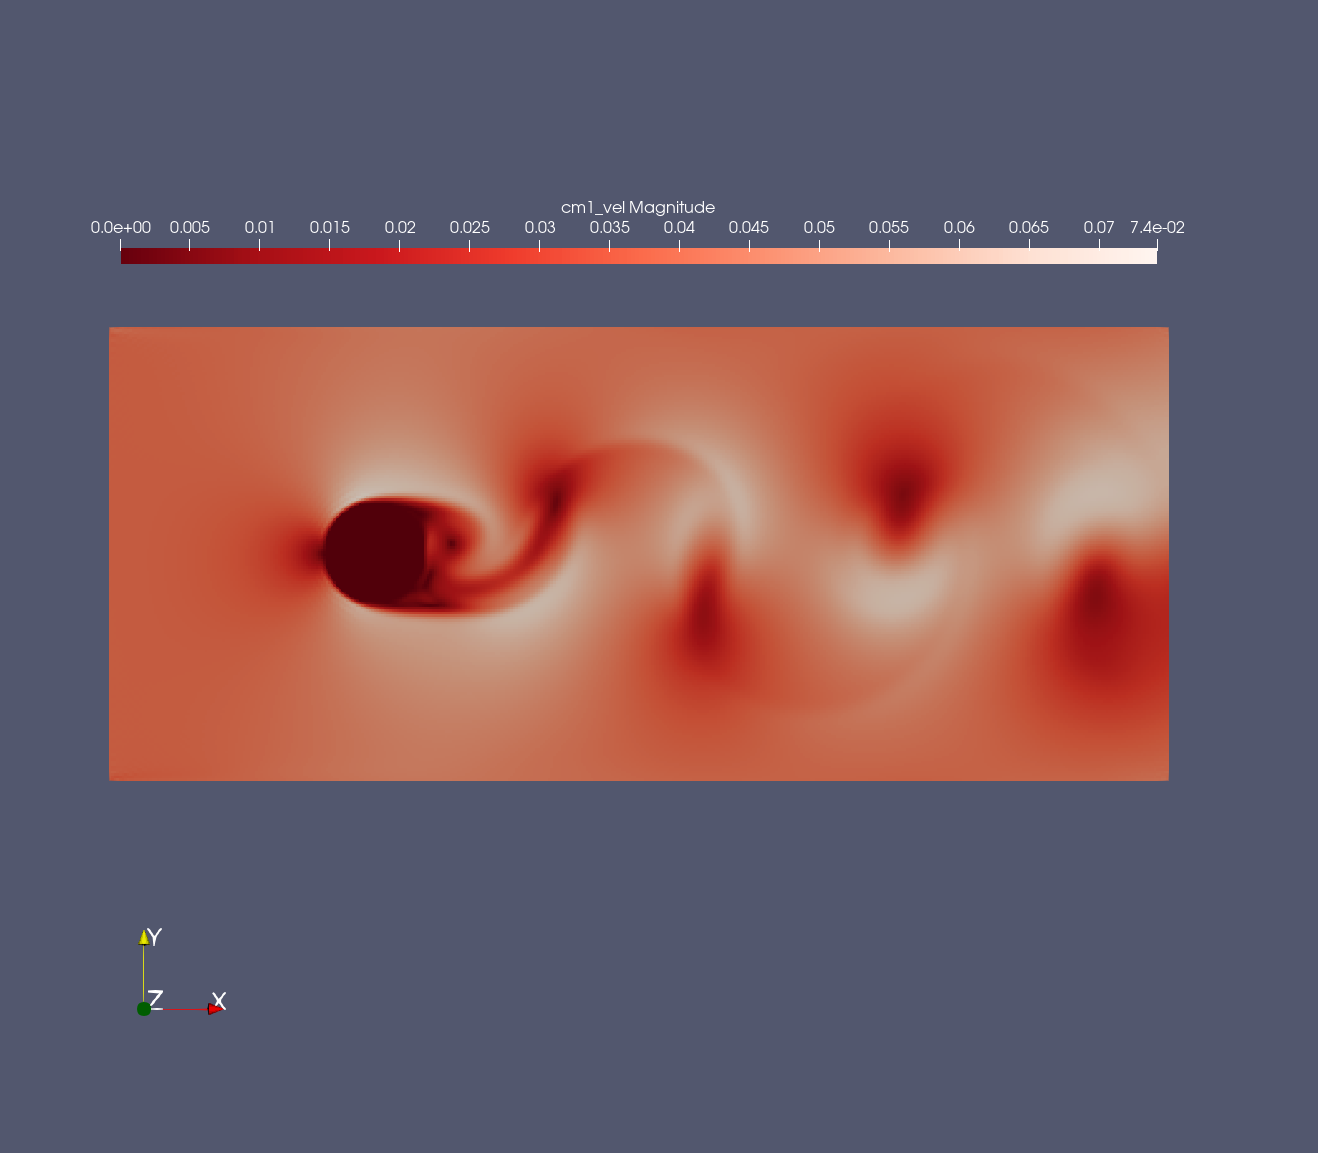
\includegraphics[width=.9\linewidth]{pics/cylinderTurbulent.png}
				\caption{Turbulent flow around cylinder}
				\label{fig:sub2}
			\end{subfigure}
			\caption{Results with direct source for quantitative comparisons.}
			\label{fig:osci}
		\end{figure}
	\end{frame}
	
	\begin{frame}{Single phase validations (qualitative)}
		\begin{figure}[h]
			\centering
			\begin{subfigure}{.5\textwidth}
				\centering
				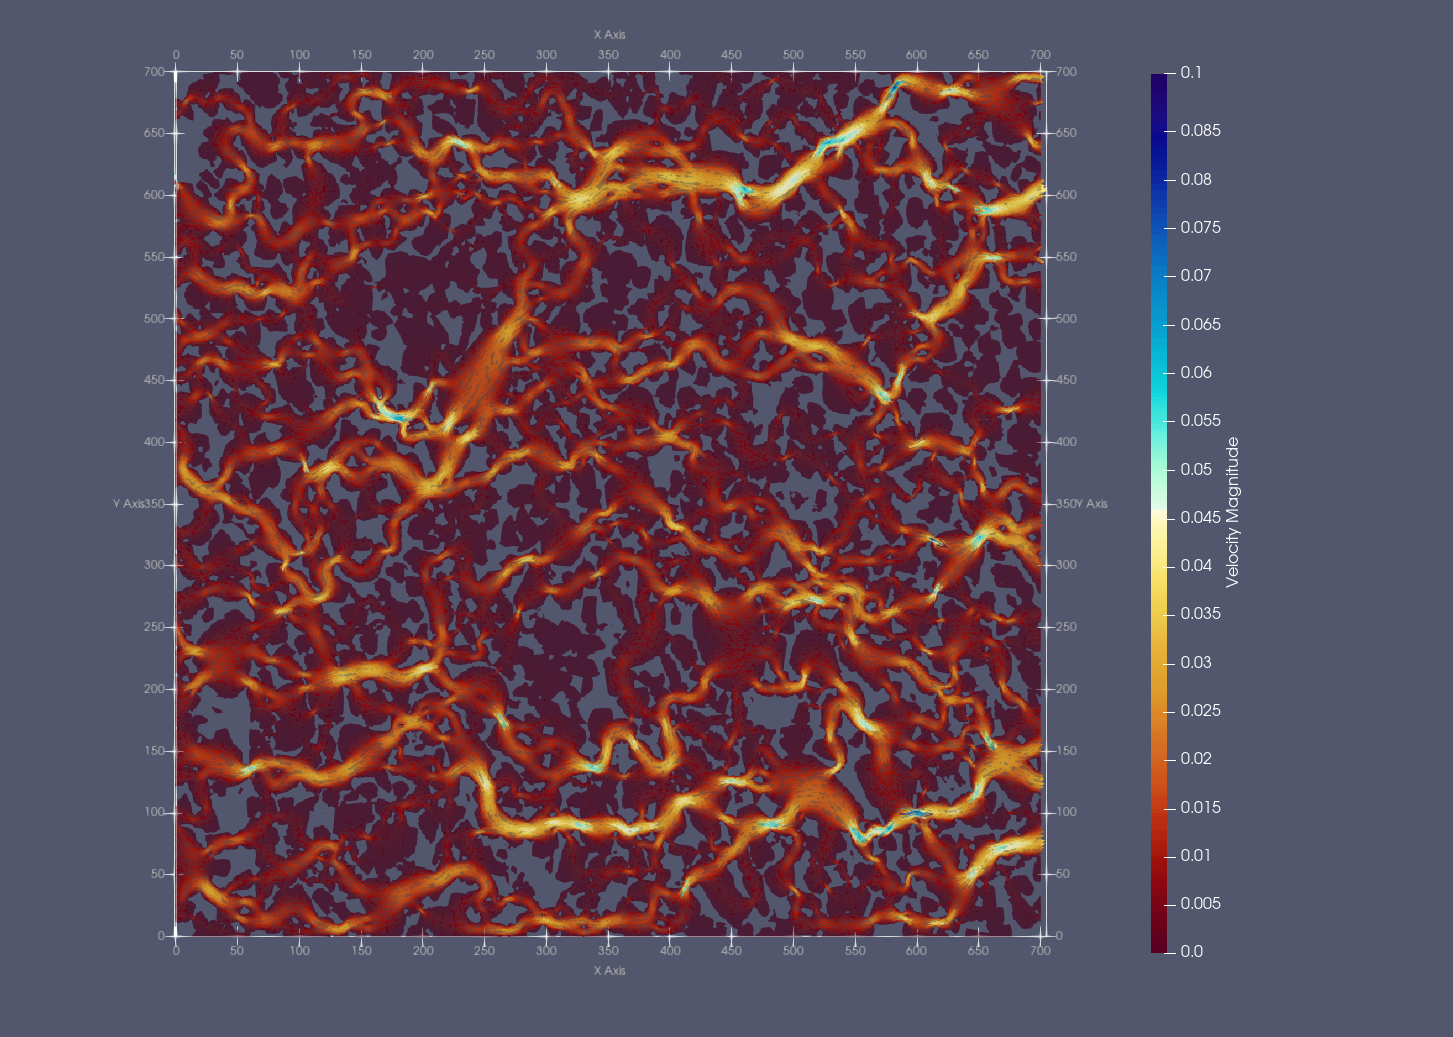
\includegraphics[width=.9\linewidth]{pics/pmVelLowV.png}
				\caption{Arbitrary porous medium (real image).}
				\label{fig:sub1}
			\end{subfigure}%
			\begin{subfigure}{.5\textwidth}
				\centering
				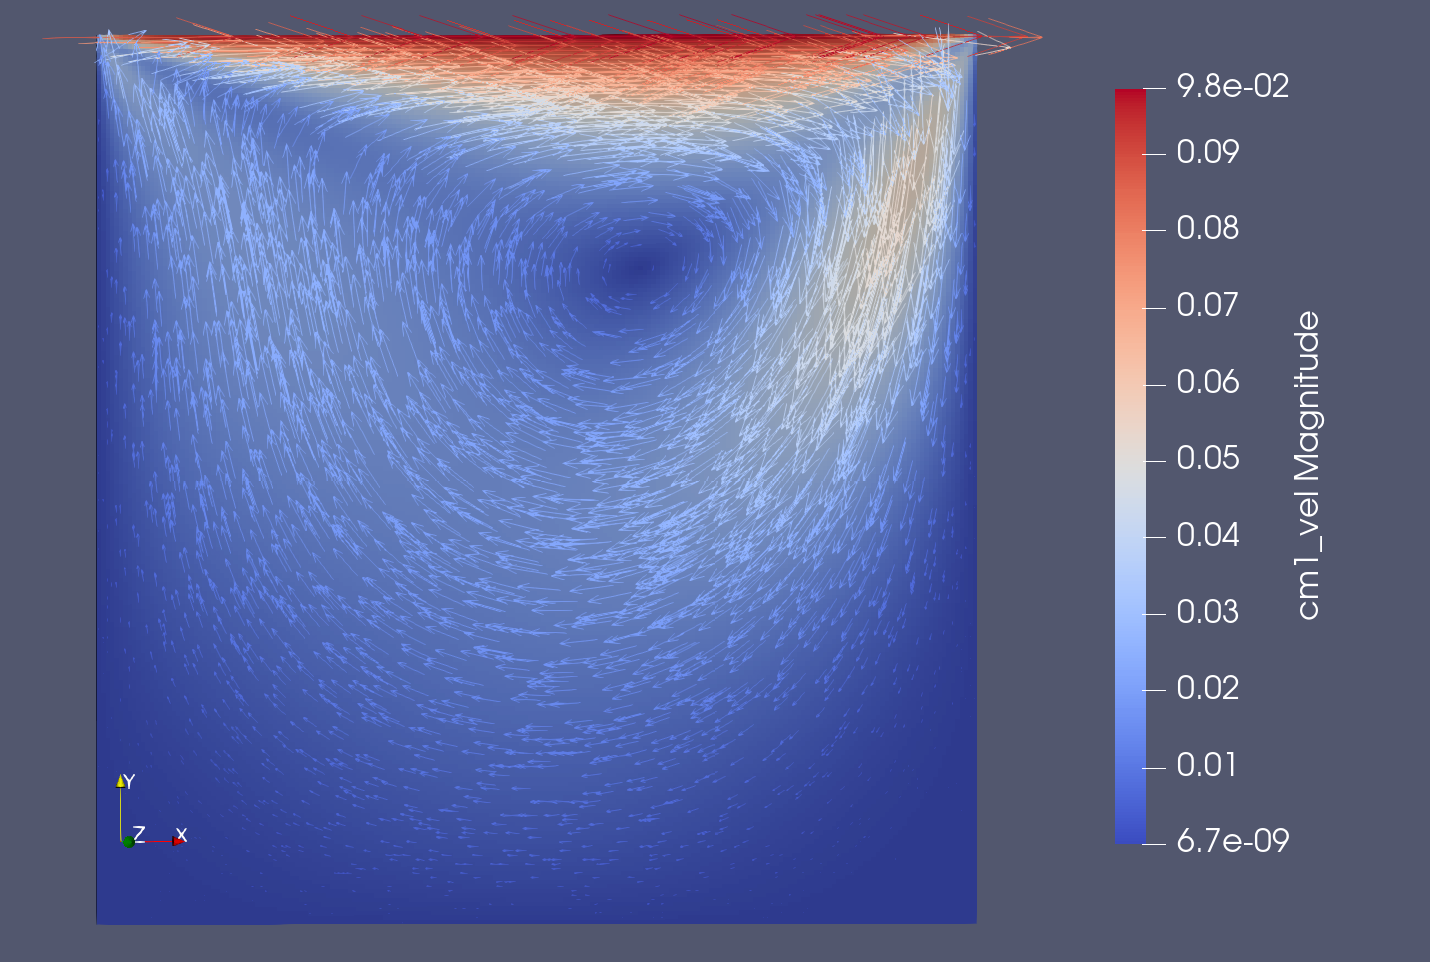
\includegraphics[width=.9\linewidth]{pics/cavity.png}
				\caption{Cavity flow, imposing a velocity on the upper wall.}
				\label{fig:sub2}
			\end{subfigure}
			\caption{Single phase cases qualitatively demonstrating the ability of modeling arbitrary porous media and arbitrary boundary conditions.}
			\label{fig:osci}
		\end{figure}
	\end{frame}

	\begin{frame}{Multiphase single component - Oscillating droplet}
		\begin{figure}[h]
			\centering
			\begin{subfigure}{.5\textwidth}
				\centering
				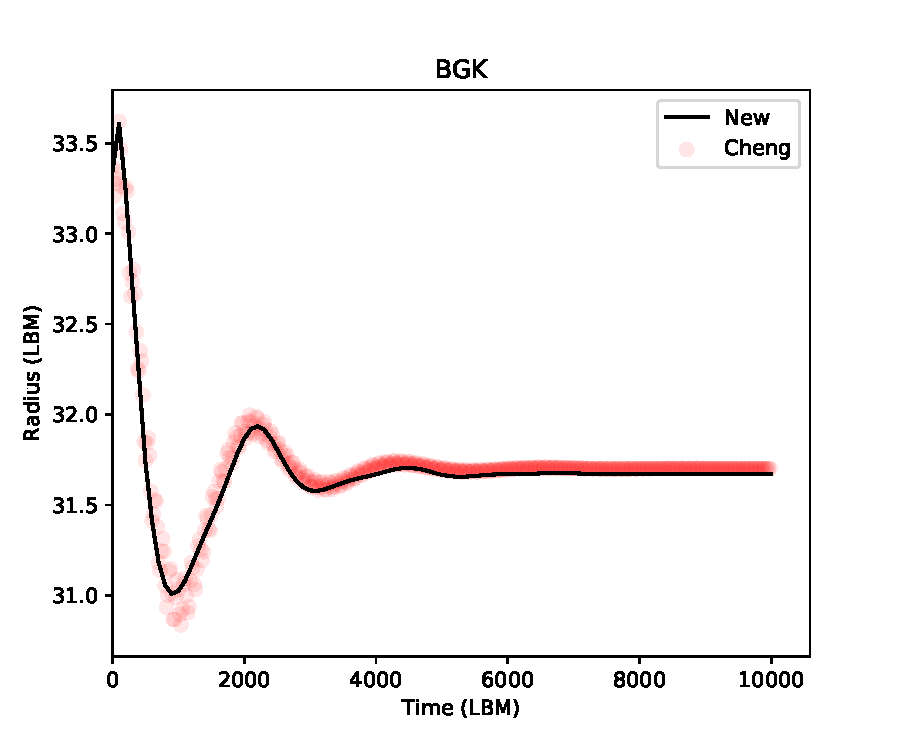
\includegraphics[width=.9\linewidth]{pics/BGKOsc.pdf}
				\caption{BGK}
				\label{fig:sub1}
			\end{subfigure}%
			\begin{subfigure}{.5\textwidth}
				\centering
				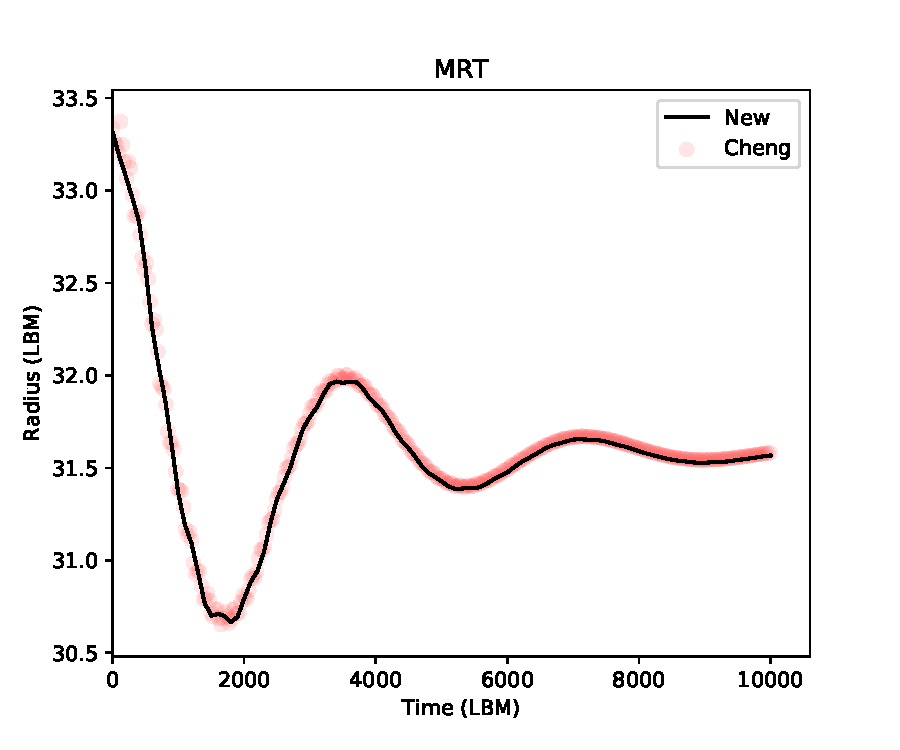
\includegraphics[width=.9\linewidth]{pics/MRTOsc.pdf}
				\caption{MRT}
				\label{fig:sub2}
			\end{subfigure}
			\caption{Oscillation droplet case. Viscosities are different in each case.}
			\label{fig:osci}
		\end{figure}
	\end{frame}
	
	\begin{frame}{Ongoing work}
		\begin{itemize}
			\item Two-component validation case
			\item Shan-Chen force in agreement with boundary conditions
			\item Viscosity per component/phase
			\item Falling and raising droplet/bubble within LBM velocity ranges (see falling droplet video).
		\end{itemize}
	\end{frame}
	
	\begin{frame}{Questions}
		\begin{itemize}
			\item<1> Mass increasing when imposing velocity/outflow.
			\begin{equation*}
			\begin{split}
				f_{i,\text{in}}^{\text{bndry}} = f_{i,\text{in}}^{\text{neighbor}} \, \, \, \text{vs.}\\
				f_{i,\text{in}}^{\text{bndry}} = f_{\bar{i},\text{in}}^{\text{bndry}} - g(\mathbf{u}_{n}^{\text{neighbor}}) \,\,\,\,\, \text{    (wall)}
			\end{split}
			\end{equation*}
			\item<1> Over-constraining P and $\mathbf{u}$ with outflow, may solve the increasing density?
			\item<2> Outflow boundary conditions. Assumptions and implications. How many layers for averaging?
			\item<2> Density variations in velocity/pressure are common in LBM?
			\item<3> Is there a general treatment for corners for all BC combinations?
			\item<3> $\Psi(P) \text{ .vs. } \Psi^i(P_i)$. Was this tried and what were the difficulties?
			\item<3> Velocity modification. Which $\tau$ to use in two-phase systems?
			\begin{equation}
			\mathbf{u}^{mod} = \mathbf{u} + \frac{\beta \mathbf{F}}{(\tau - 0.5)\psi^2}
			\end{equation}
		\end{itemize}
	\end{frame}

	\begin{frame}{Density variations}
		\begin{columns}
			\column{0.5\textwidth}
			\begin{figure}
				\centering
				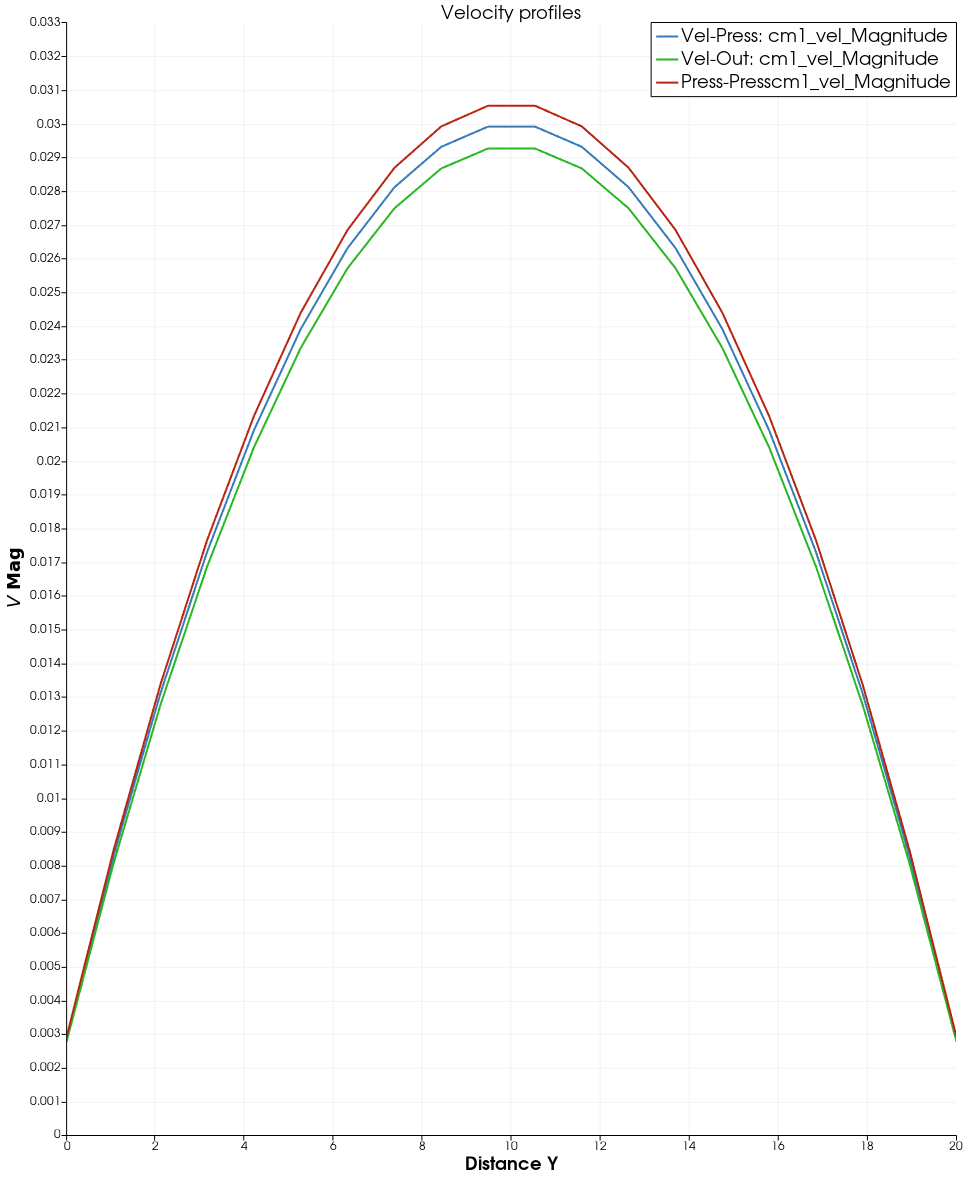
\includegraphics[width=\textwidth]{pics/velDropBox.png}
				%\caption[]{}    
				\label{}
			\end{figure}
			
			\column{0.5\textwidth}
			
			\begin{figure}
				\centering
				
				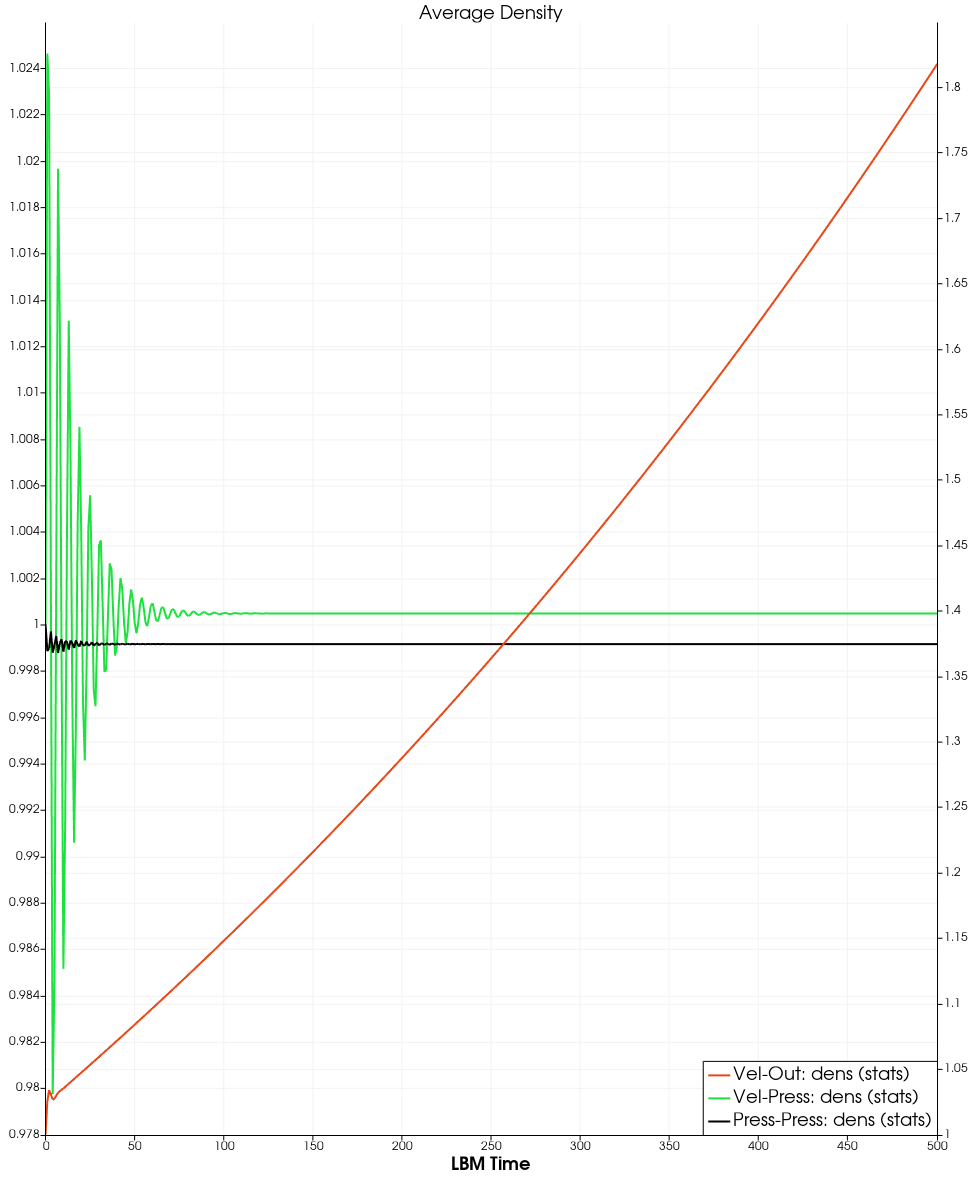
\includegraphics[width=0.8\textwidth]{pics/globalDenBox.png}
				%\caption[]{}   
				\label{}
			\end{figure}
		\end{columns}
	\end{frame}
	
	\begin{frame}{\href{https://www.overleaf.com/project/5f5cfacb13ed640001eeb63d}{\color{green}Paper}}
		
		What cases were selected for validation?\\~\\
		
		Ideas/tasks for dynamic validations:
		\begin{itemize}
			\item Young-Laplace equation
			\item Find analytical expression for oscillation frequency
			\item Rayleigh-Taylor instability (surface waves)
			\item Rising bubble/falling droplet (simple analytical solution in 3D!)
			\item Impacting droplet
		\end{itemize}
	
	Starting with the Young-Laplace case is straightforward, if this case will go in the paper.
	\end{frame}
	
	\begin{frame}{Discussion}
		Discussion...
	\end{frame}
	%---------------------------------------------------------
	%---------------------------------------------------------
	%---------------------------------------------------------
	%---------------------------------------------------------
	%---------------------------------------------------------
	%---------------------------------------------------------
	%---------------------------------------------------------
	%---------------------------------------------------------
	%---------------------------------------------------------
	
	\begin{frame}{Input}
		\begin{figure}
			\centering
			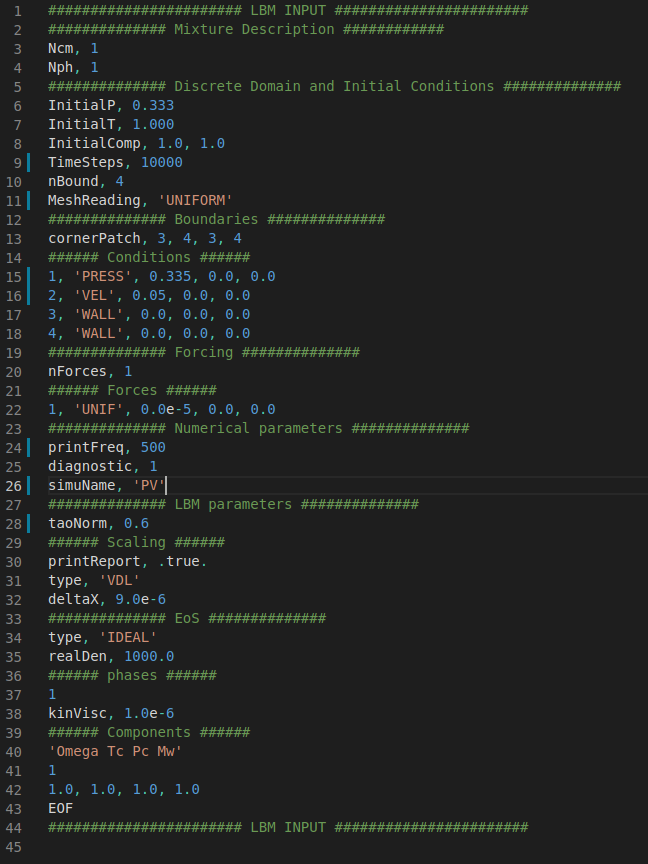
\includegraphics[width=0.5\textwidth]{pics/modelInput.png}
		\end{figure}
	\end{frame}
	
	\begin{frame}{Discussion}
		Discussion...
	\end{frame}
	
	\begin{frame}{Actions}
		\begin{itemize}
			\item Explore the use of outflow condition with combinations of other impositions at the inlet
			\item Detect the source of the mass increase. Outlet? Inlet?
			\item Extend column of fluid for the falling droplet simulation
			\item Repeat the rotating droplet case
			\item Lamb's Book
			\item Previous paper in the group
			\item William's experience with boundary conditions
			\item Which Fortran version is recommended?
		\end{itemize}
	\end{frame}
	
	%---------------------------------------------------------
	%---------------------------------------------------------

	\subsection*{Report Feb 28 - 2022}
	\label{}
	\justifying
	\begin{frame}
		\textbf{Report Feb 28 - 2022}\\~\\
		Actions:
		\begin{itemize}
			\item Teams as file-sharing platform
			\item Git tutorial to General folder and convert it into an Overleaf file
			\item Migrate bibliography to Teams
			\item Suggested books in a list in General
			\item What is the device name to draw on Windows desk?
		\end{itemize}
	
	\begin{block}{Question}
		Which papers to upload? Decide first nomenclature?
	\end{block}

	CODE-YEAR-CATEGORY-NAME-FIRSTAUTHORNAME-JOURNAL
	\end{frame}


	%---------------------------------------------------------
	%---------------------------------------------------------
	
	\subsection{Weekly meeting - LBM - Mar 11 - 2022}
	\label{}
	\justifying
	\begin{frame}{Weekly meeting - LBM}
		\textbf{Mar 11 - 2022}\\~\\
		\begin{itemize}
			
			\item Outflow boundary conditions
			\item Two-components implementation

		\end{itemize}
	\end{frame}
	
	\begin{frame}{Boundary conditions}
		In the previous meeting, I raised some questions regarding the combination of boundary conditions. To clarify those points, the following was done:
		
		\begin{itemize}
			\item A channel with closed boundaries was simulated under three combinations of BC.
			\item Velocity/Outflow, Velocity/Pressure, and Pressure/Pressure, were tested.
			\item The velocity profile at two locations, and the fluxes at boundaries were computed\footnote{The fluxes are actually measured half way from the real boundary.}
		\end{itemize}
	\end{frame}
	
	\begin{frame}{Boundary conditions}
		
		Moving wall (using average density)/ Velocity BC:
		\begin{equation*}
		f_{i}(\mathbf{x}_b,t+\delta t) = f^*_{i^-}(\mathbf{x}_b,t) - 2 w_i \rho_w \frac{\mathbf{c}_{i^-} \cdot \mathbf{u}_w}{c_s^2}
		\end{equation*}
		Pressure condition (interpolating velocity):
		\begin{equation*}
		f_{i}(\mathbf{x}_b,t + \delta t) = - f^*_{i^-}(\mathbf{x}_b,t) + 2 w_i \rho_w \left[1+\frac{(\mathbf{c}_{i^-} \cdot \mathbf{u}_w)^2}{2c_s^4} - \frac{\mathbf{u}^2_w}{2c^2_s} \right]
		\end{equation*}
		Local $\rho$ for open boundaries, and global $\rho$ for static walls.\\
		{\color{red}
			Mistakes:\\
			Outflow (1): Interpolating velocity from adjacent layer and use wall BC\\
			Outflow (2): Copying distribution functions from adjacent layer. }
		
	\end{frame}
	
	
	\begin{frame}{Boundary conditions}
		
		Animation.
		\begin{figure}
			\centering
			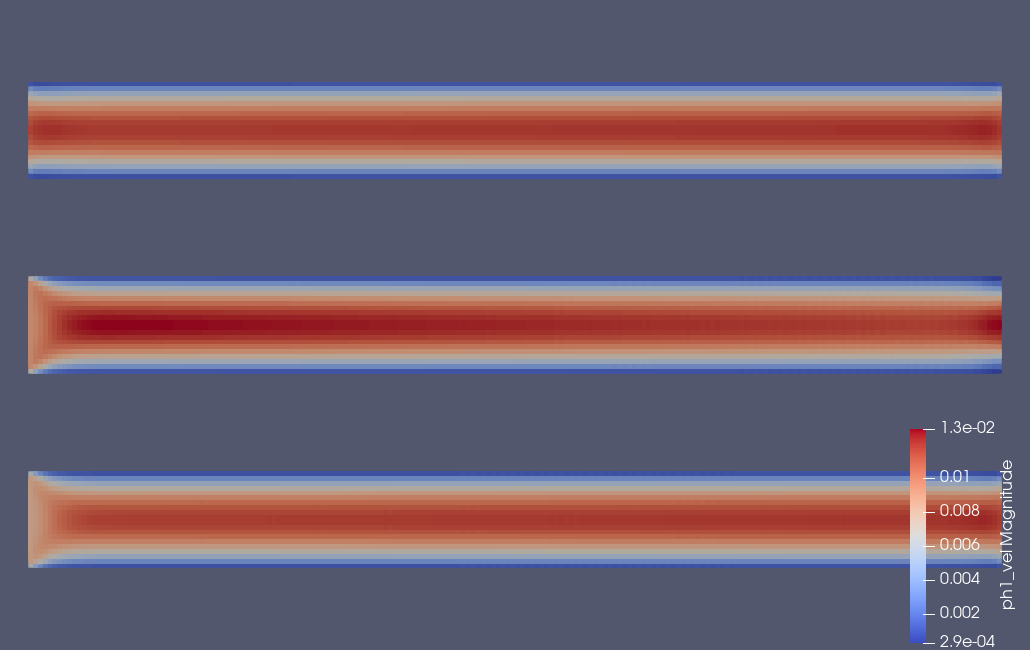
\includegraphics[width=0.75\textwidth]{pics/channelBCComparision.png}
		\end{figure}
	\end{frame}
	
	\begin{frame}{Boundary conditions}
		\begin{figure}
			\centering
			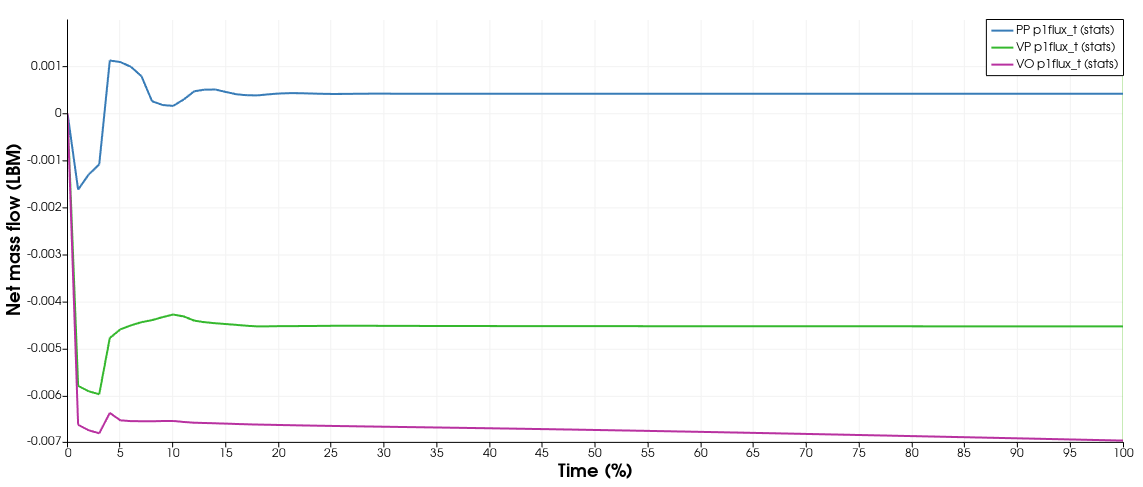
\includegraphics[width=0.75\textwidth]{pics/channelBCComparisionNetFlow.png}
		\end{figure}
		\begin{figure}
			\centering
			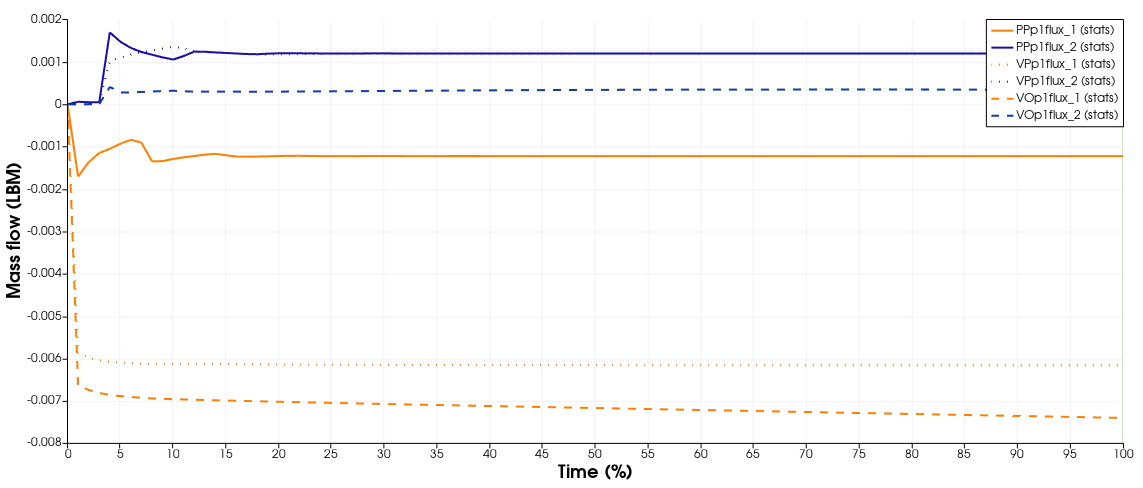
\includegraphics[width=0.75\textwidth]{pics/channelBCComparisionBndFlow.png}
		\end{figure}
			
	\end{frame}

	\begin{frame}{Partial conclusions}
		\begin{itemize}
			\item Outflow requires some corrections to agree with CBC, Zou-He, William's findings.
			
			\item Pressure/Pressure does not depict a transition of the boundary layer. Positive/negative impact on multiphase flow?
			
			\item Velocity/boundary is not conserving mass with current implementations. The effect is reduced considerably, interpolating the velocity and applying the moving wall BC.
			
			\item These cases will be the benchmark for outflow implementations, and will provide the answer if the mass increasing problem is solved by doing the proposed corrections.  
		\end{itemize}
	\end{frame}
	
	
	\begin{frame}{Two-components results}
		Regarding the two-components implementation (the main objective to address the dynamic simulations) this was performed:
		
		\begin{itemize}
			\item The mixing rule for viscosity was implemented (falling droplet keeps accelerating)
			\item Programmed initialization of arbitrary composition or density fields (concentration fields creates peaks in density profile)
			\item Corrected some incompatibilities between EoS, type of force, and initialization method.
			\item Two tested cases: static and oscillating droplet
		\end{itemize}
	\end{frame}
	
	\begin{frame}{Two-components results}
		\begin{figure}
			\centering
			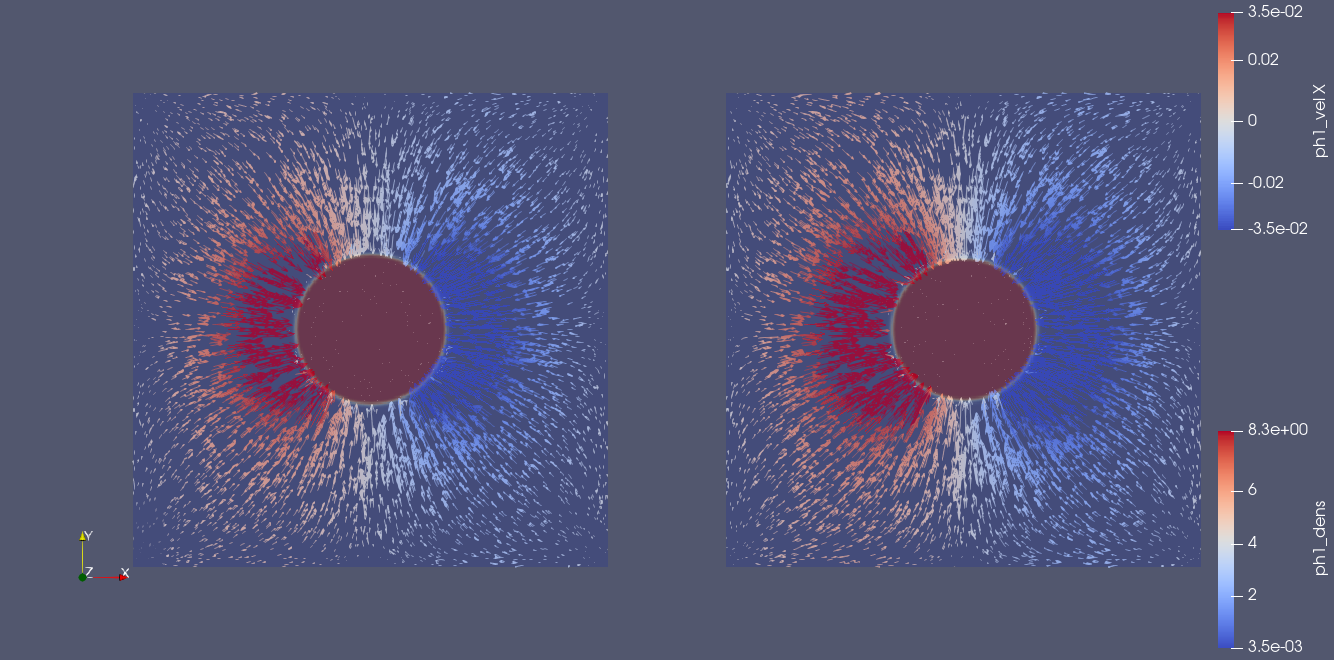
\includegraphics[width=0.60\textwidth]{pics/TwoCMP_MRT_StaticvsOsc.png}
		\end{figure}
	
		\begin{figure}
			\centering
			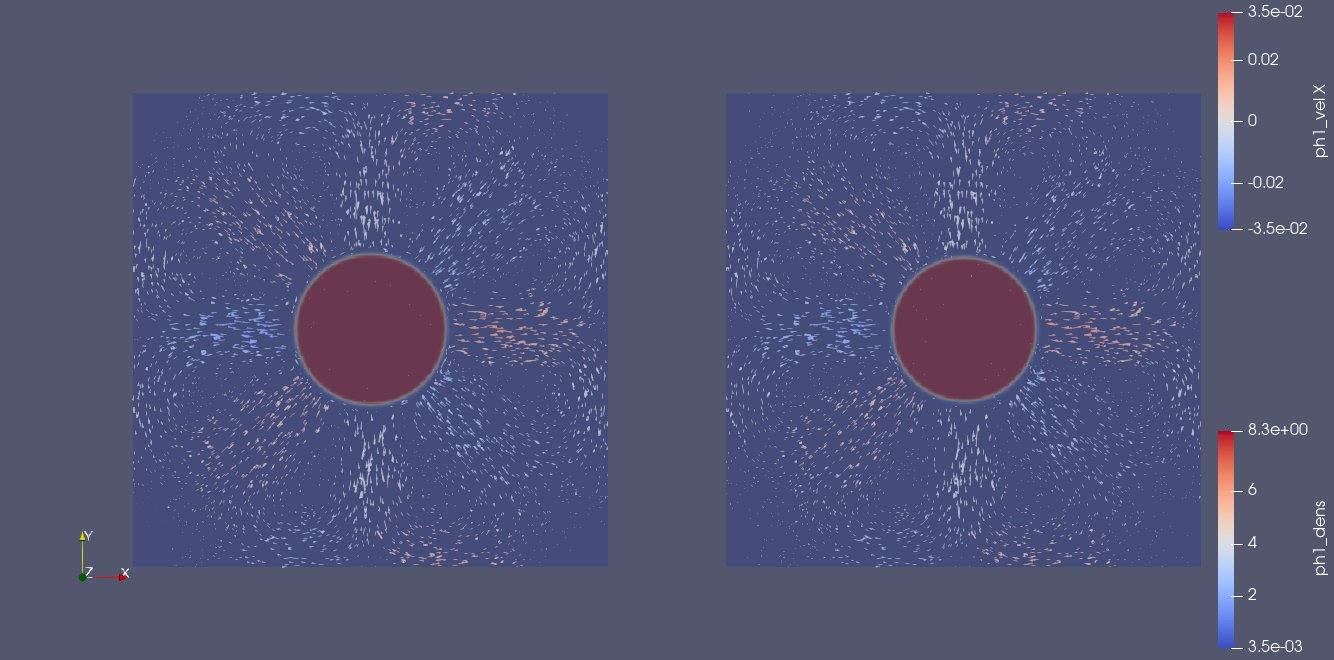
\includegraphics[width=0.6\textwidth]{pics/TwoCMP_MRT_StaticvsOscEq.png}
		\end{figure}
	\end{frame}

	\begin{frame}{Two-components results}
		
		Minor and major axes oscillations. These are not validated results. They only reflect the expected behavior of the droplet.
		\begin{figure}
			\centering
			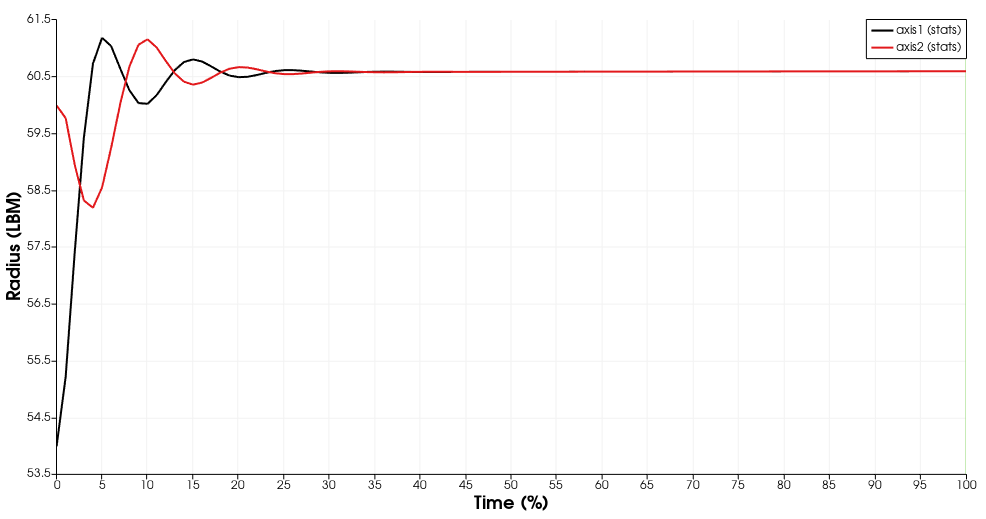
\includegraphics[width=0.9\textwidth]{pics/TwoCMP_MRT_OscRadius.png}
		\end{figure}
	\end{frame}

	\begin{frame}{Partial conclusions}
		
		Coding tasks:
		\begin{itemize}
			\item The force needs to be generalized for non-periodic BCs. 
			\item Pressure, velocity (and symmetric) boundaries have to be generalized for the multi-component case.
			\item Change falling droplet for raising bubble (allows for modifying the external viscosity to slow down the bubble.)
			\item Fortran version?
		\end{itemize}
	
		~\\Theoretical tasks:
		\begin{itemize}
			\item Dig deeper into bibliography (Lamb's book) to obtain the analytical solutions
			
		\end{itemize}
	\end{frame}
	
	\begin{frame}{Actions}
	\begin{itemize}
		\item Stay in oscillation case and obtain the comparison
		\item Initialize with a different radius (stabilized)
		\item Can we impose composition and pressure to eliminate peaks?
		\item Run case with radius higher than stabilized
		
		\item Read papers referencing Lamb's equation for analytical comparison
	\end{itemize}
	\end{frame}

	%---------------------------------------------------------
	%---------------------------------------------------------
	\subsection{Weekly meeting - LBM - Mar 24 - 2022}\label{meet:LBM00324}
	\label{}
	\justifying
	\begin{frame}{Weekly meeting - LBM}
		\textbf{Mar 24 - 2022}\\~\\
		\begin{itemize}
			
			\item Dynamic validation: oscillating droplet
			\item Next dynamic cases: raising bubble - splashing droplet
			
		\end{itemize}
	\end{frame}
	
	\begin{frame}{Oscillating droplet}
		\textbf{Indications from the last meeting...}\\~\\
		\begin{itemize}
			\item Initialize droplet with different radii
			\item Find papers referencing Lamb's equation
		\end{itemize}
		
		
		~\\ Done during these weeks:
		\begin{enumerate}
			\item Static simulations to obtain $R_e$ and $\Delta p$, and thus compute $\sigma$
			\item Dynamic oscillation. $R_e$ was obtained, along with the oscillation period $T_n$.
		\end{enumerate}
	
	\end{frame}
	
	\begin{frame}{Static results - Young Laplace}
		$P_c = \frac{\sigma}{r}$, for a 2D geometry.
		$\sigma = $ 0.12141. Here, $r = R_e$, the equilibrium radius.
		
		\begin{figure}[h]
			\centering
			\begin{subfigure}{.5\textwidth}
				\centering
				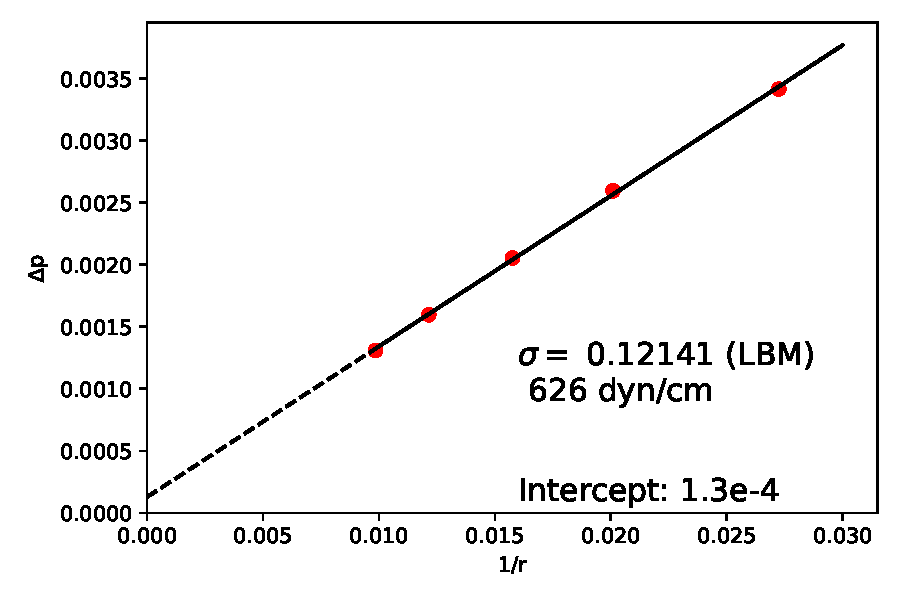
\includegraphics[width=1\linewidth]{pics/IFT.pdf}
				\caption{Young-Laplace validation}
			\end{subfigure}%
			\begin{subfigure}{.5\textwidth}
				\centering
				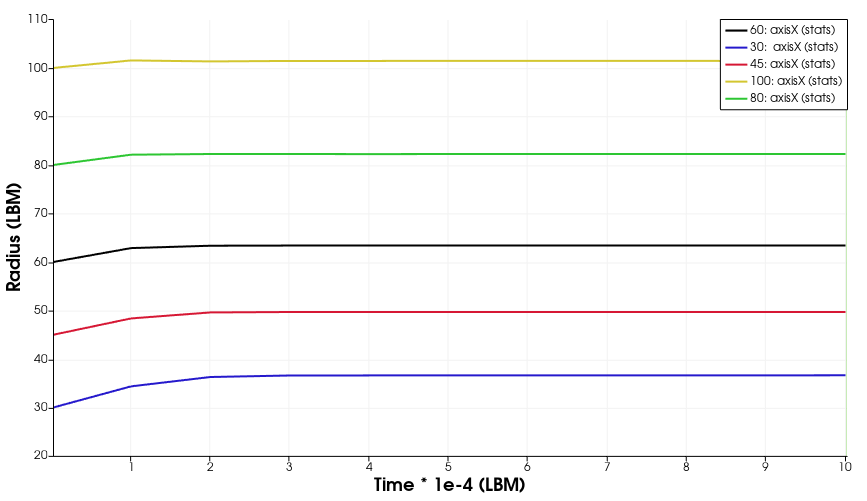
\includegraphics[width=1\linewidth]{pics/2c_staticRChange.png}
				\caption{Evolution of $R_e$ for the static cases.}
			\end{subfigure}
			\caption{Young Laplace and $R_e$ change due to thermodynamic inconsistency.}
			\label{fig:laplace}
		\end{figure}
		 
	\end{frame}
	
	\begin{frame}{Oscillating droplet}
		$R_{x,0} = 60, R_{y,0} = 0.9 R_{x,0}$, in a grid of 400x400. $\tau_l = \tau_v = 0.56$, to reduce the viscous dissipation.
		\begin{figure}[h]
			\centering
			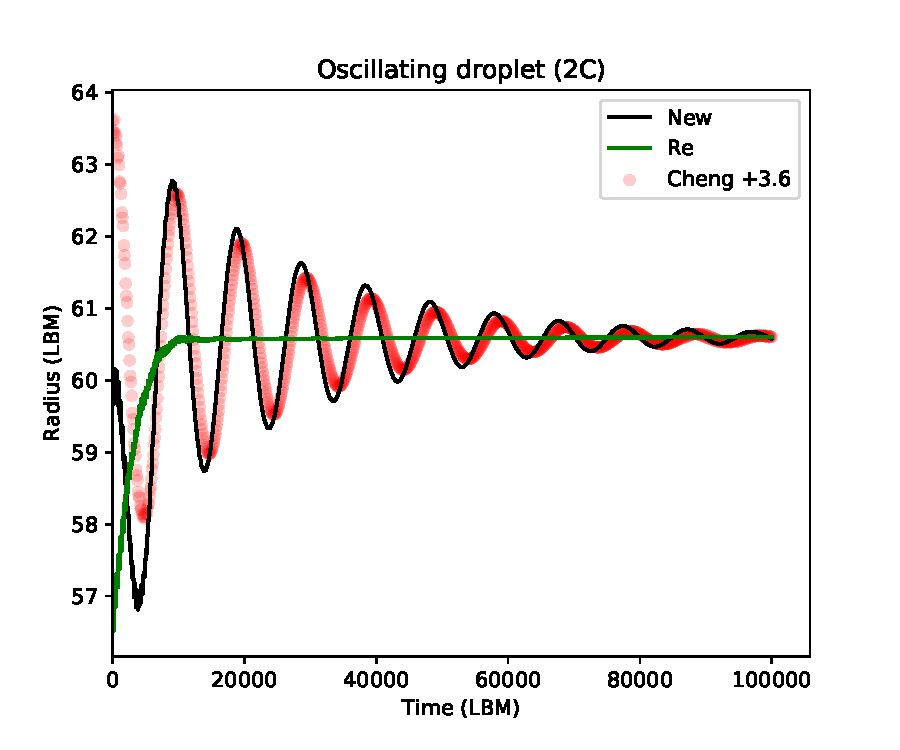
\includegraphics[scale=0.4]{pics/2cOsc.pdf}
			\caption{Oscillation of the X axis compared with Cheng's solution.}
			\label{fig:2cOsc}
		\end{figure}
	\end{frame}
	
	\begin{frame}{Fourier transform}
		
		\begin{columns}
			
			\column{0.5\textwidth}
			\begin{figure}[h]
				\centering
				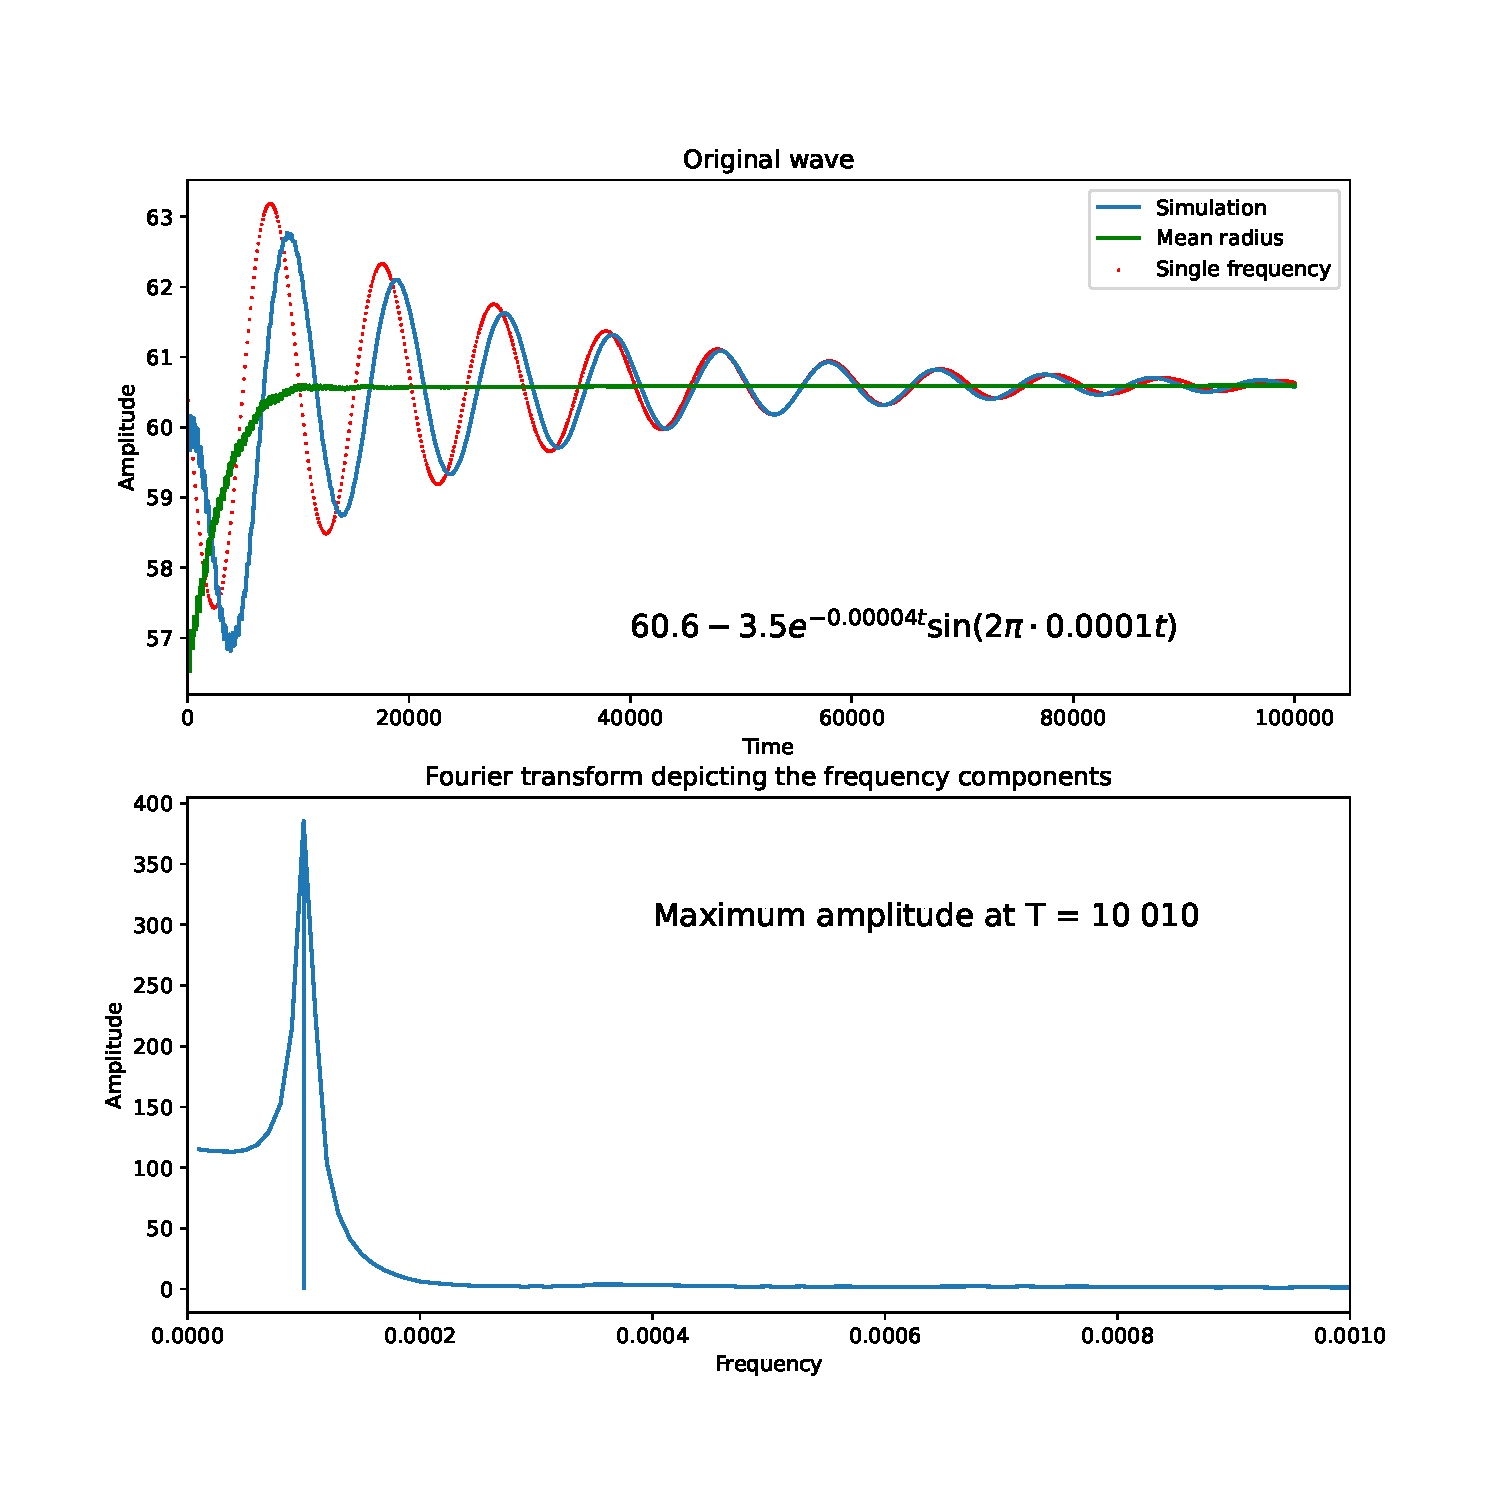
\includegraphics[width=1\linewidth]{pics/fourier.pdf}
				\caption{Maximum amplitude at $T_n = 10010$.}
				\label{fig:2cOsc}
			\end{figure}
			
			\column{0.5\textwidth}
			Analytical solution:
			\begin{equation}
			T_a = 2 \pi \left[ \frac{n (n^2-1) \sigma}{\rho_l R_e^3} \right]^{-0.5}
			\end{equation}
			
			Giving a period $T_a = $ 9989. This gives a relative error of 2\%. 
			
		\end{columns}
		
		
	\end{frame}
	
	\begin{frame}{Conclusions and questions}
		
		\begin{itemize}
			\item<1> The oscillation period has been matched successfully with the analytical solution.
			\item<1> The first oscillation is masked by a thermodynamic inconsistency, what causes the droplet to increase its radius, at the cost of decreasing the vapor density. This is my hypothesis for the change in equilibrium radius, and not that the initial interface profile is providing additional energy to the system.
			\item<2-> Things that could be done if further analysis is required:
			\begin{itemize}
				\item Calibrate $\beta$ and $\kappa$ to remove the inconsistency (this only would improve the prediction during first oscillation.)
				\item The jump magnitude of the radius is dependent on the grid size:\\
				 200x200 42.8 to 43.6 (0.8)\\
				 300x300 42.8 to 45.3 (2.5).
			\end{itemize}
		\end{itemize}
	\end{frame}
	
	\begin{frame}{Next dynamic cases - Raising bubble}
				
		\begin{columns}
			
			\column{0.5\textwidth}
			Expectations:
			\begin{itemize}
				\item Test two simultaneous forces. Gravity:
				\begin{equation*}
					\mathbf{F}_g = \mathbf{g} (1- \frac{<\rho>}{\rho})
				\end{equation*}
			\end{itemize}
			
			Validations:
			\begin{itemize}
				\item Bubble shape as a function of Bond and Reynolds numbers.
				\item Terminal velocity (Reynolds number).
			\end{itemize}
			\column{0.5\textwidth}
			Implications:
			\begin{itemize}
				\item Implement the gravity force
				\item At the small scale given by the use of $a$ and $b$, how small the gravity turns to be? My preliminary calculation is $\mathbf{g}_{LBM} = 6.31 e-14$, compared with interaction forces of 1e-1.
			\end{itemize}
		\end{columns}
		~\\~\\
		{\tiny Sankaranarayanan K., Shan X., Kevrekidis I.G., and Sundaresan S. Analysis of drag and virtual mass forces in bubbly suspensions using an implicit formulation of the lattice Botlzmann method.}
	\end{frame}
	
	\begin{frame}{Next dynamic cases - Splashing droplet}
		
		\begin{columns}
			
			\column{0.5\textwidth}
			Expectations:
			\begin{itemize}
				\item Validate the $beta$ model at several density ratios and Reynolds values
				\item Implement the symmetric BC for the top
				\item Implement the solid-fluid interaction
			\end{itemize}
			
			Validations:
			\begin{itemize}
				\item Cheng's and other published results
				\item Droplet shape and boundaries
			\end{itemize}
			\column{0.5\textwidth}
			Implications:
			\begin{itemize}
				\item Test the solid-fluid interactions (although this has minor effect)
				\item Test implementation of other BC than periodic for two components.
			\end{itemize}
		\end{columns}
	\end{frame}
	
	
	\begin{frame}{Actions}
		\begin{itemize}
			\item
		\end{itemize}
	\end{frame}

	%---------------------------------------------------------
	%---------------------------------------------------------
	\subsection{Report - Mar 28 - 2022}
	\label{}
	\justifying
	\begin{frame}{}
		\textbf{Report - Mar 28 - 2022}\\~\\
		\begin{itemize}
			
			\item Cheng's paper
			\item Dynamic cases
			\item Questions about thermodynamics
			
		\end{itemize}
	\end{frame}

	\begin{frame}{Cheng's paper}
		\begin{itemize}
			\item Source of dissipation: increasing radius, not tested using $\kappa$ (source term in MRT),  everyone else is still using it (credibility).
			\item Oscillations (I will keep record of a bibliographic search to study how to present this result).
			\item Looking at a more fine time-resolution, the droplet increases its radius after 1000 iterations, first in the right side, and then to the left side. The increase is not high (within the size of the interface) but still think it should not happen. 

			
		\end{itemize}
	\end{frame}

	\begin{frame}{Dynamic cases}
		\begin{itemize}
			\item Rising bubble. I have not found a case using periodic boundary conditions. Preliminary results: bubble accelerates, the droplet and its interface are stable. I did not bring pictures to first address the appropriateness of my approach to this case.
			
		\end{itemize}
	\end{frame}

	\begin{frame}{Questions about thermodynamics}
		
		\begin{equation*}
		\left(\frac{\partial \ln \phi_i}{\partial P}\right)_{T,N} = \frac{\bar{v}_i}{RT} - \frac{1}{P}
		\end{equation*}
		
		\begin{itemize}
			\item Saturation pressure and temperatures.	
			\item Does it have any meaning the inverse of the partial molar volume and what would be the implication of using it as an splitting coefficient?
		\end{itemize}
	\end{frame}


	\begin{frame}{Actions}
		\begin{itemize}
			\item Read bibliography about oscillations of other authors
			\item Read Cheng's reports and decide for which case replicate for validation
			\item Which $a,b$ from EOS regime can be simulated for the rising bubble?
			\item Oscillation case is done. It's important to recognize the reason for the increasing radius.
			\item Math about what it would mean to split according to the partial molar volume. 
			\item Partial molar properties for general cases!
			
		\end{itemize}
	\end{frame}
	
	%---------------------------------------------------------
	%---------------------------------------------------------
	\subsection{Report - Apr 11 - 2022}
	\label{}
	\justifying
	\begin{frame}{}
		\textbf{Report - Apr 11 - 2022}\\~\\
		\begin{itemize}
			\item PNG 510
			\begin{itemize}
				\item Method of characteristics
				\item Laplace transform
				\item Partially miscible displacement (analytical solution)
			\end{itemize}
			\item PNG 520
			\begin{itemize}
				\item Usage of Rachford-Rice equation for different purposes
				\item Doubt with Raoult's law (ideal solution)
				\item Generative function $\frac{g^R}{RT}$
			\end{itemize}
			\item EME 521
			\begin{itemize}
				\item SPH fundamentals 
				\item Boundary conditions
			\end{itemize}
			\item PNG 501
			\begin{itemize}
				\item Generalization of fractional flow with the presence of capillarity and gravity
			\end{itemize}
			\item Qualifying exam
		\end{itemize}
	\end{frame}

	\begin{frame}{Actions}
		\begin{columns}
			
			\column{0.5\textwidth}
			
			
			\column{0.5\textwidth}
			
		\end{columns}
	\end{frame}
	
	%---------------------------------------------------------
	%---------------------------------------------------------
	
	\subsection{Report - Apr 18 - 2022}
	\label{}
	\justifying
	\begin{frame}{}
		\textbf{Report - Apr 18 - 2022}\\~\\
		\begin{itemize}
			\item Asymmetry fixed in LBM (videos. Highlight case that diverges (high shear?))
			\item Presentation with simulation setup
			\item Read well-balanced LBM 
			\item PBM. Doubt about increasing in cell moles due to decreasing in $M_w$.
			\item Comment about SPH
		\end{itemize}
	\end{frame}
	
	\begin{frame}{Actions}
		\begin{columns}
			
			\column{0.5\textwidth}
			Search SPH + Porous Media Applications\\
			Replicate the error case where density decreases but the molecular weight makes the molar density higher.\\
			\textbf{Note}: the Cahn-Hilliard macroscopic equation can be integrated into Navier-Stokes by multiple forms. Muzammil is working on integrating the solution via external force, and solve one PDF per component. Others, have solved the Cahn-Hilliard via finite-element methods, while solving a single PDF for two components, or solving $n_c-1$ CH to obtain order parameters + 1 PDF to recover NS. Another approach: solve an LBM that recovers CH, and then proceed solving a single PDF for NS.\\
			
			\column{0.5\textwidth}
			Assumptions behind the parachor approximation, also for multiphase mixtures.\\
			How well-balaned LBM affects scaling. Does it give an extra degree of freedom?\\
			\textbf{Shan-Chen pseudopotential used in literature to replicate results}\\
			Compile readings and gravity implementations.\\
			Read cases in multiphase book.
			
			
		\end{columns}
	\end{frame}
	
	%---------------------------------------------------------
	%---------------------------------------------------------
	\subsection{LBM Meeting - Apr 22 - 2022}
	\label{meet:LBM00422}
	\justifying
	\begin{frame}{LBM Meeting}
		\textbf{Apr 22 - 2022}\\~\\
		Recap from last meeting (see \ref{meet:LBM00324}):
		\begin{itemize}
			\item The oscillating droplet case was validated against the analytical solution
			\item The thermodynamic inconsistency usually compromises the vapor density.
		\end{itemize}
		
		Today:
		\begin{itemize}
			\item Raising bubble physics
			\item Related studies
			\item Simulation setup and results (single component)
			\item Simulation setup and results (multicomponent)
		\end{itemize}
	\end{frame}
	
	
	
	\begin{frame}{Raising bubble physics}
		
		\begin{columns}[T]
		
			\column{0.5\textwidth}
			
			\begin{itemize}
				\item Main properties
				\begin{itemize}
					\item Surface tension
					\item Body forces
					\item Viscosity and density ratio
					\item Boundary conditions
				\end{itemize}
			
				\item Bond and Morton numbers fix $R_e = \frac{u_t d_b}{\nu_l}$
				\begin{equation*}
				\begin{split}
				B_o = \frac{g \Delta \rho d_b^2}{\sigma}\\
				M_o = \frac{g \Delta \rho \mu_l^4}{\sigma^3 
					\rho_l^2}
				\end{split}
				\end{equation*}
				
				\item The drag coefficient, $C_D$, function of $R_e$, and defined as: 
				\begin{equation*}
				\begin{split}
				C_D = \frac{4 \Delta \rho g d_b}{3 u_t^2 \rho_l}
				\end{split}
				\end{equation*}
				resulting from a drag and gravity force balance. 
				\end{itemize}
		
			\column{0.5\textwidth}
			\begin{figure}
				\centering
				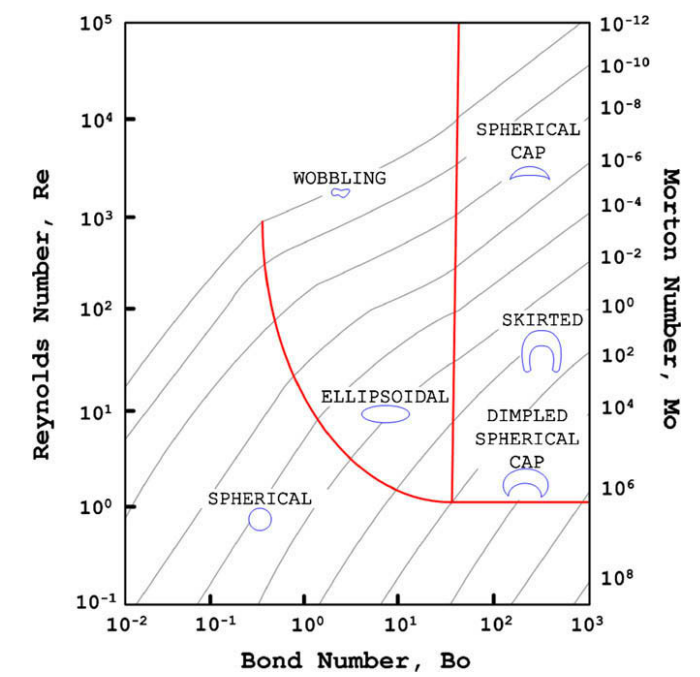
\includegraphics[scale=0.2]{pics/shapeRegimes.png}
				\\{\tiny \justifying Taken from Amaya-Bower L., Lee T. Single bubble rising dynamics for moderate Reynolds number using Lattice Boltzmann Method. Computer and Fluids. 2010.}
			\end{figure}
			
		\end{columns}
		
	\end{frame}

	\begin{frame}{Experimental relationship of $C_D$ with $R_e$}
		
		The constants may change due to the 2D approximation. 
		\begin{figure}
			\centering
			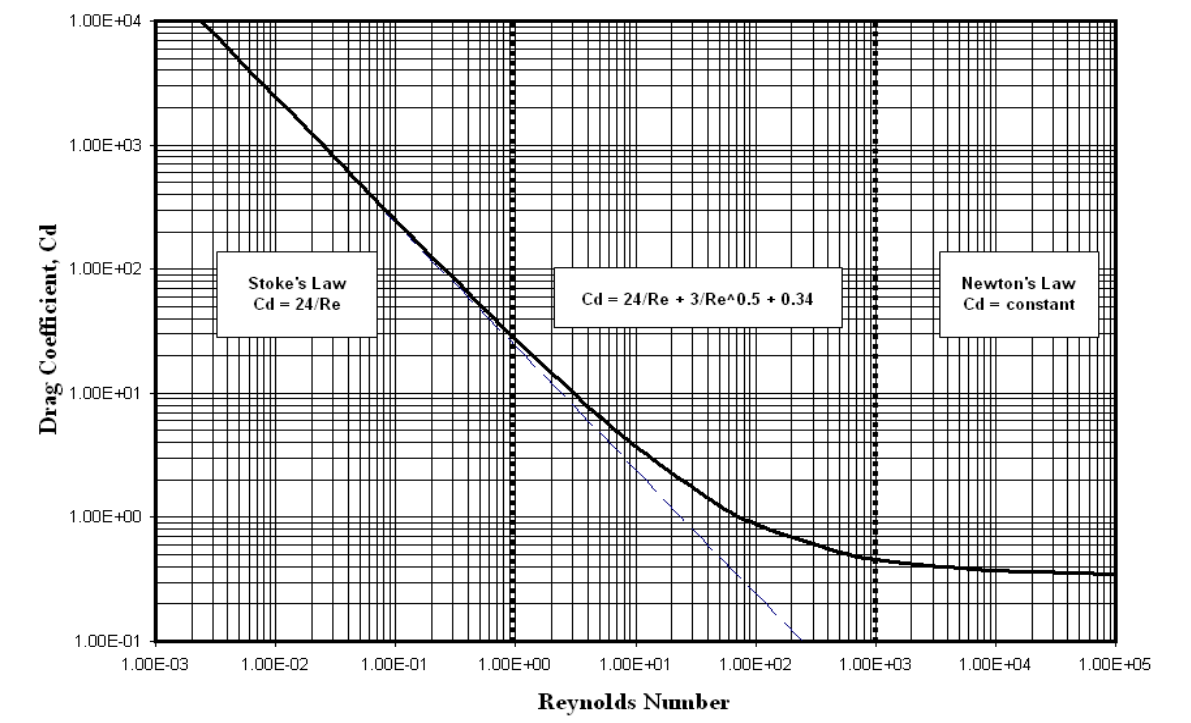
\includegraphics[scale=0.2]{pics/dragRe.png}
			\\{\tiny \justifying Taken from API Specifications for Oil and Gas Separators and PNG 480 Handout. L. Ayala, H. Emami-M. }
		\end{figure}
	\end{frame}
	
	\begin{frame}[t]{Considerations}
		\justifying
		
		\begin{columns}[T]
			
			\column{0.45\textwidth}
			\textbf{Goal}~\\
			\justifying
			
			Test the pseudopotential approach for partially misc. mixtures, under the action of gravity.\\~\\
			
			\textbf{Methodology}~\\
			Test different flow regimes based on Bond (Eotvos) and Morton numbers. Validate against \textbf{terminal velocities and bubble shapes.}
			
			\begin{equation*}
			R_e = \frac{\rho_l u_b d_b}{\mu_l}
			\end{equation*}
			\begin{equation*}
			B_o = \frac{g \Delta \rho d_b^2}{\sigma} \,\,\,\, 	M_o = \frac{g \Delta \rho \mu_l^4}{\sigma^3 
				\rho_l^2}
			\end{equation*}
			
			
			A thermodynamic state fixes $\rho, \Delta \rho, \sigma$. At a given temperature, in a single component case, some values are provided ($\rho, \Delta \rho$) and others can be obtained by simulating the static droplet ($\sigma$). \\
			
			\column{0.45\textwidth}{
				\justifying
				
			}
			
			\textbf{Procedure}	
			\begin{itemize}
				\item Select $B_o$
				\item Calculate the gravity $g = \frac{B_o \sigma}{\Delta \rho d_b^2}$
				\item Select $M_o$
				\item Calculate $\mu_l^4 = \frac{M_o \sigma^3 \rho_l^2}{g \Delta \rho }$
				\item Select the viscosity ratio
				\item Calculate $\mu_g = \mu_l * \frac{\mu_g}{\mu_l}$
			\end{itemize}
			
			The LBM parameters are thus fixed:

			\begin{equation*}
			\begin{split}
			\tau = \frac{\nu}{c_s^2}+ \frac{\Delta t}{2}
			\end{split}
			\end{equation*}
			
			\textbf{Try single component and then the multicomponent case.}
		\end{columns}
	\end{frame}
	
	\begin{frame}{Related studies}
		\textbf{Amaya-Bower L, Taehun L. 2010.}~\\
		\begin{itemize}
			\item LBM (modified to remove acoustic waves) with Cahn Hilliard (recovered through second PDF).
			\item Closed domain in 2D and 3D.
			\item Evaluate dependency to:
			\begin{itemize}
				\item Grid resolution. They recommend $d_b$ = 40.
				\item Domain size. $4d_b$x$9d_b$.
				\item $\mu$ ratio $>$ 100 to reach $u_t$
				\item Gravity force implementation. No difference between $-g (\rho-\rho_r) \nabla h$ and $-g \rho \nabla h$. 
			\end{itemize}  
		\end{itemize}
		~\\
		\textbf{Sankaranarayanan, K., Shan X., Kevrekidis, I.G., and Sundaresan S. 2002.}~\\
		\begin{itemize}
			\item Two-component model. 
			\item Periodic domain in 3D. $\mathbf{a} = g(1-\frac{\tilde{\rho_r}}{\rho})$
			\item Contributions to our work:
			\begin{itemize}
				\item Uses van der Waals for 1 component and ideal for the second one
				\item Shows 2D results depicting wiggling by unstable conditions
				\item Suggests an implicit scheme, that seems to be still local
				\item Closure problem for upscaling drag between phases
				\item Stands the difficulty to achieve high $B_o$, while keeping low $M_o$
			\end{itemize}  
		\end{itemize}
	%https://www-sciencedirect-com.ezaccess.libraries.psu.edu/science/article/pii/S0301932222000106#fig0005
	
	%https://www-sciencedirect-com.ezaccess.libraries.psu.edu/science/article/pii/S1290072921000466?via%3Dihub
	\end{frame}
	
	
	\begin{frame}[t]{Simulation setup (Amaya)}
		\justifying
		\begin{columns}[t]
			\column{0.45\textwidth}
			
			\textbf{Domain}: (!) 200x360 mesh (2D)\\
			\textbf{Fluid}: Water at 485.33 K ($T_r$ = 0.75), and $P_r$ = 0.092. \\$\rho_l^0$  = 7.679 (), $\rho_v^0$  = 0.109. $\rho_L/\rho_g$ = 70. $\tau_l$ = 210.5. $\tau_g$ = 0.8. $\mu_l/\mu_g$ =10.\\~\\
			Initial condition: Spherical droplet with $d_o$ = 40, and $w_o$ = 8.
			
			~\\
			\textbf{Boundary conditions}: No-slip condition on all boundaries.
			
			~\\
			\textbf{Parameters}: Shan-Chen $G$=-1.0. \\
			Beta = 0.9\\
			Time = 10000 ($\approx 10 \sqrt{\frac{d_b}{g}}$)\\
			~\\
			
			
		
			\column{0.45\textwidth}
			
		
			\textbf{Single static simulation}:\\ $\Delta \rho $ = 7.2 (7.7-0.5), $d_s$ = 40.0, \\ $\Delta P$ = 8.5e-3 - 5.87e-3 = 2.623e-3 \\$\sigma = \Delta P \cdot r$ = 0.05254.\\
			
			
			First, the single component case was tested as follows:
			\begin{enumerate}
				\item $B_o$ = 1. $M_o$ = 3e-5. $\mu_R$ = 100. 
				\item $B_o$ = 10. $M_o$ = 2e-2. $\mu_R$ = 10.
				\item $B_o$ = 10. $M_o$ = 2e-2. $\mu_R$ = 100. 
				\item $B_o$ = 0.1. $M_o$ = 1e-2. $\mu_R$ = 100.
				\item $B_o$ = 22. $M_o$ = 8.4e-4. $\mu_R$ = 100. 
			\end{enumerate}
		\end{columns}
	\end{frame}
	
	\begin{frame}{Preliminary Results}
		\begin{figure}
			\centering
			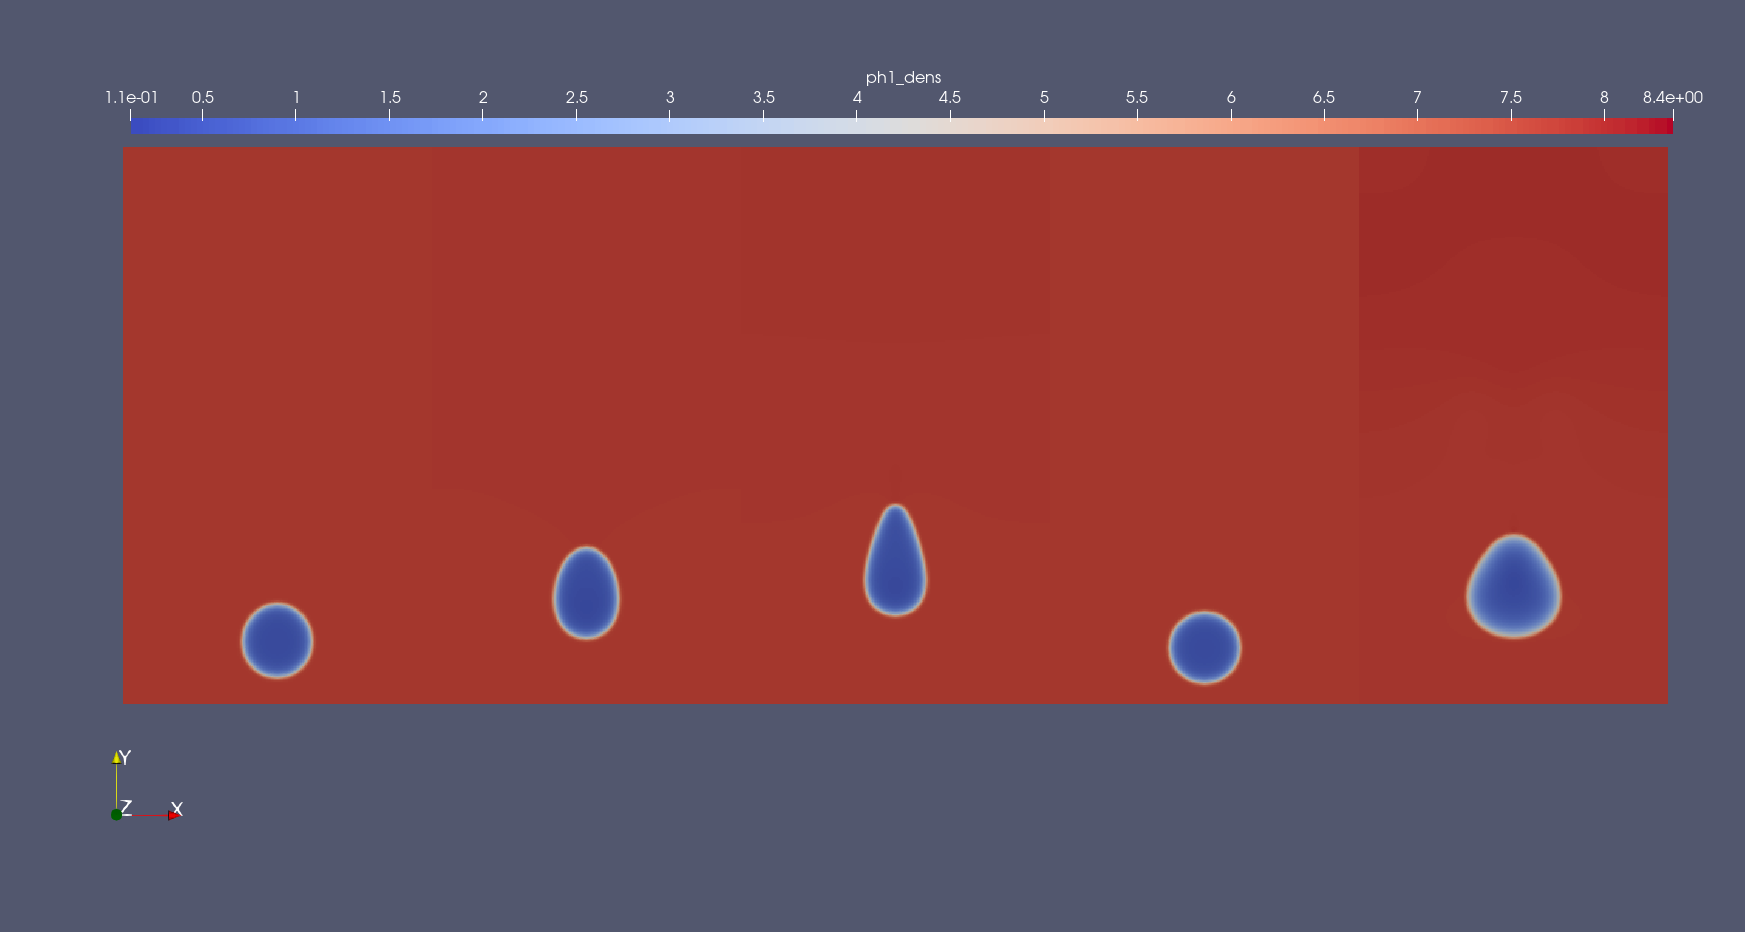
\includegraphics[scale=0.2]{pics/risingCompDen.png}
			\\{\tiny \justifying Bubble shapes}
		\end{figure}
	\end{frame}

	\begin{frame}{Preliminary Results}
		\begin{figure}
			\centering
			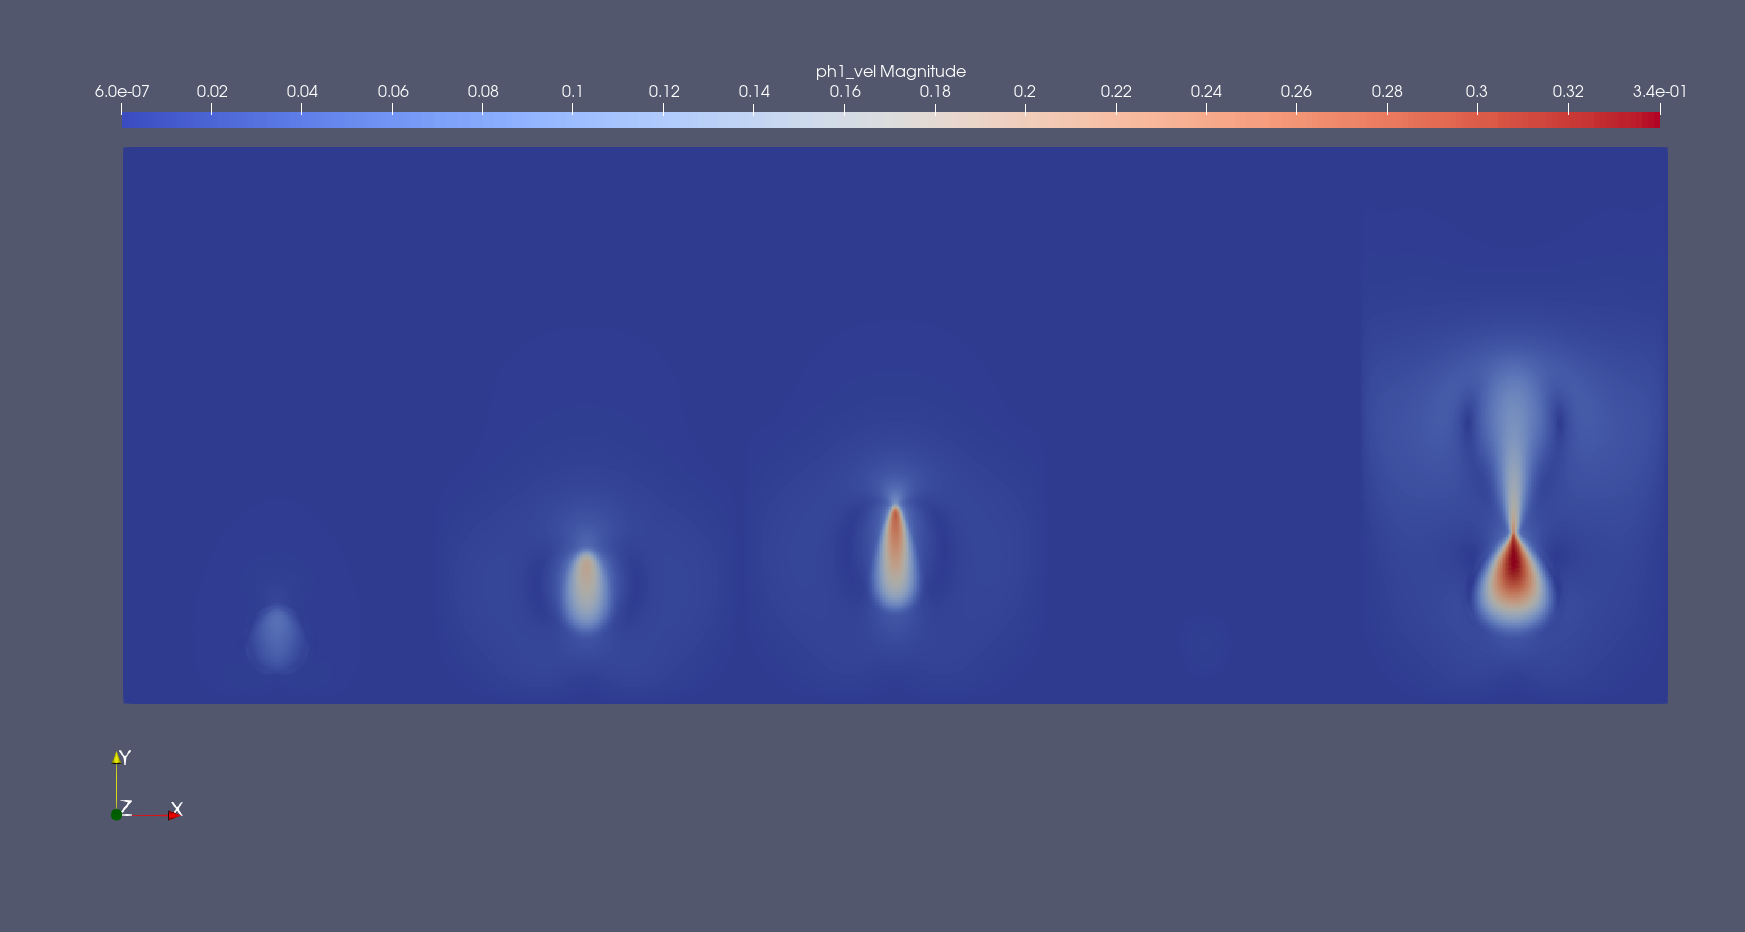
\includegraphics[scale=0.2]{pics/risingCompVel.png}
			\\{\tiny \justifying Velocity field}
		\end{figure}
	\end{frame}

	\begin{frame}{Difficulties in single phase}
		\textbf{}\\~\\
		\begin{itemize}
			\item Reach low Morton values (due to restrictions in kinematic viscosity).
			\item Reach high Bond numbers (high gravity)
			\item The cap shapes are not being observed, and the ellipsoidal tends to be more triangular.
			\item Hard to change Bond with fixed $\sigma$. System becomes unstable with other values of $G$.
		\end{itemize}
	\end{frame}
		
		
	\begin{frame}{Increasing the Morton number}
		Trying to make the liquid more viscous (at $B_o$ = 10), seems to not allow the bubble to rise ($M_o$ = 8e6), which later collapses.\\~\\
		\begin{itemize}
			\item $\tau_g$ = 0.52. $\tau_l$ = 47
			\item $\tau_g$ = 2.0. $\tau_l$ = 47 
			\item $\tau_g$ = 0.92. $\tau_l$ = 4.7 
		\end{itemize}
		\begin{figure}
			\centering
			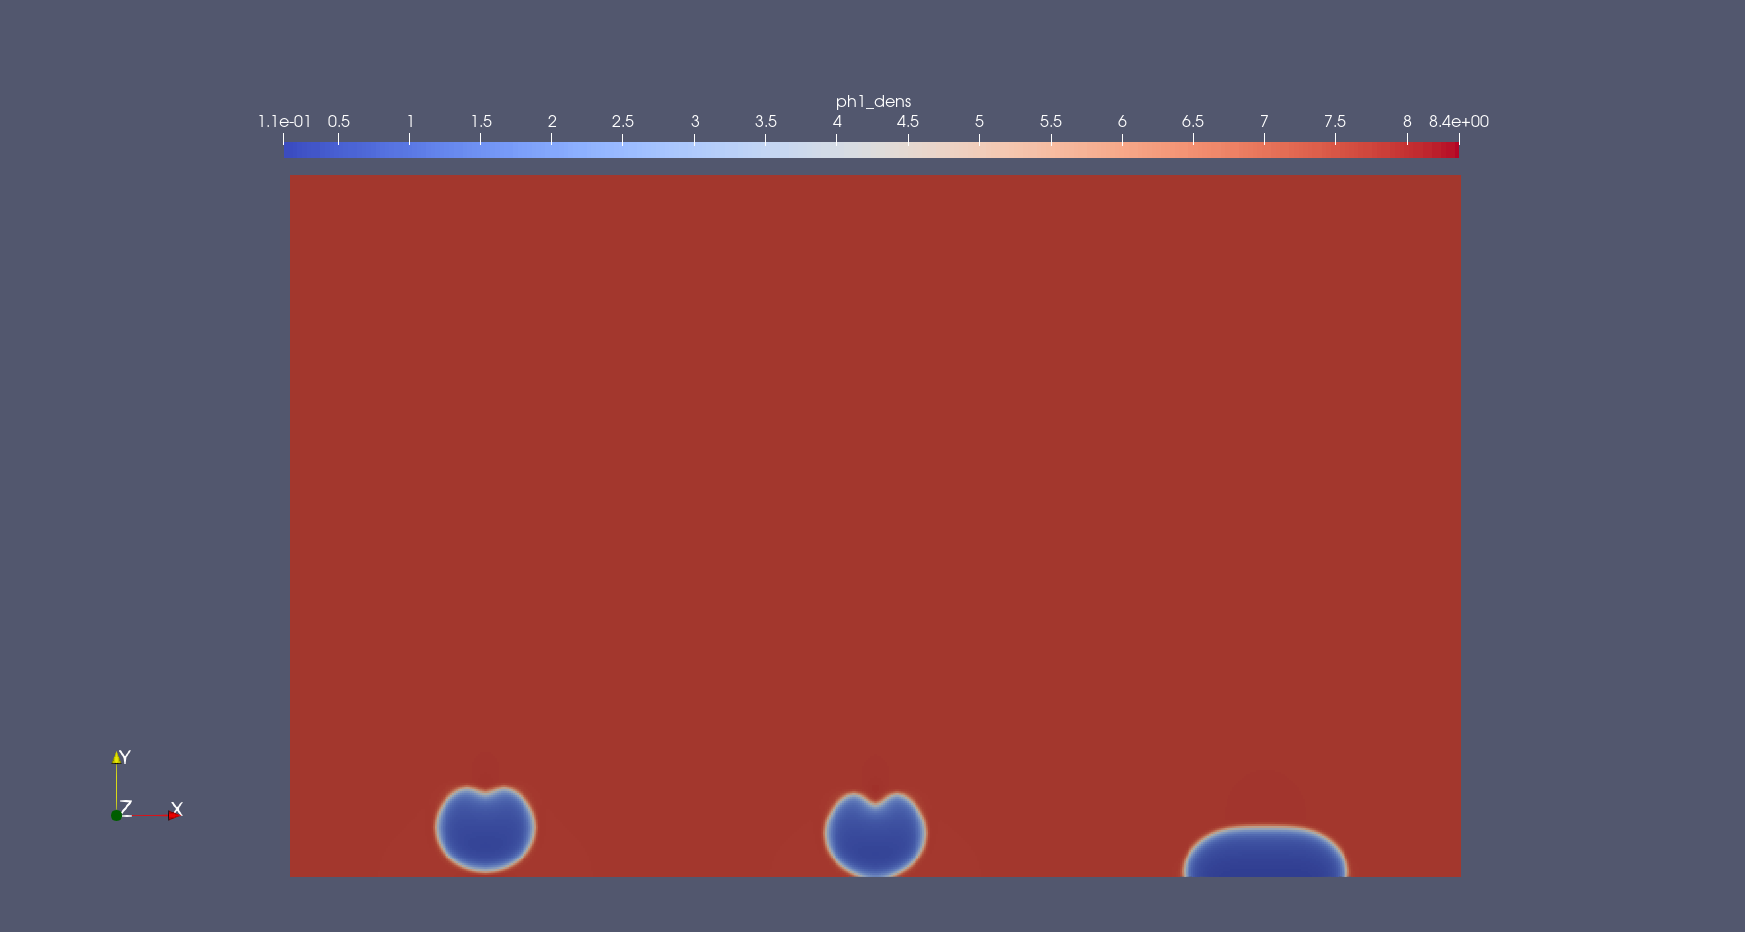
\includegraphics[scale=0.15]{pics/risingCompDen456.png}
			\\{\tiny \justifying Velocity field}
		\end{figure}
	\end{frame}

	\begin{frame}{Potential solutions}
		\textbf{}\\~\\
		\begin{itemize}
			\item Fix MRT parameters
			\item Consider an implicit scheme
			\item Compare against the usual Shan-Chen force which may provide better stability 
		\end{itemize}
	\end{frame}
	
	\begin{frame}{Multicomponent case - First approach}
		\textbf{MC case with the beta model}\\~\\
		Using the same mixture that was used for the oscillating droplet, with a viscosity ratio of 10, two cases were run:
		\begin{itemize}
			\item $B_o$ = 10, $M_o$ = 5e-3.
			\item $B_o$ = 10, $M_o$ = 5e-4.
		\end{itemize}
	\end{frame}
	\begin{frame}{Multicomponent case - First approach}
		\begin{figure}
			\centering
			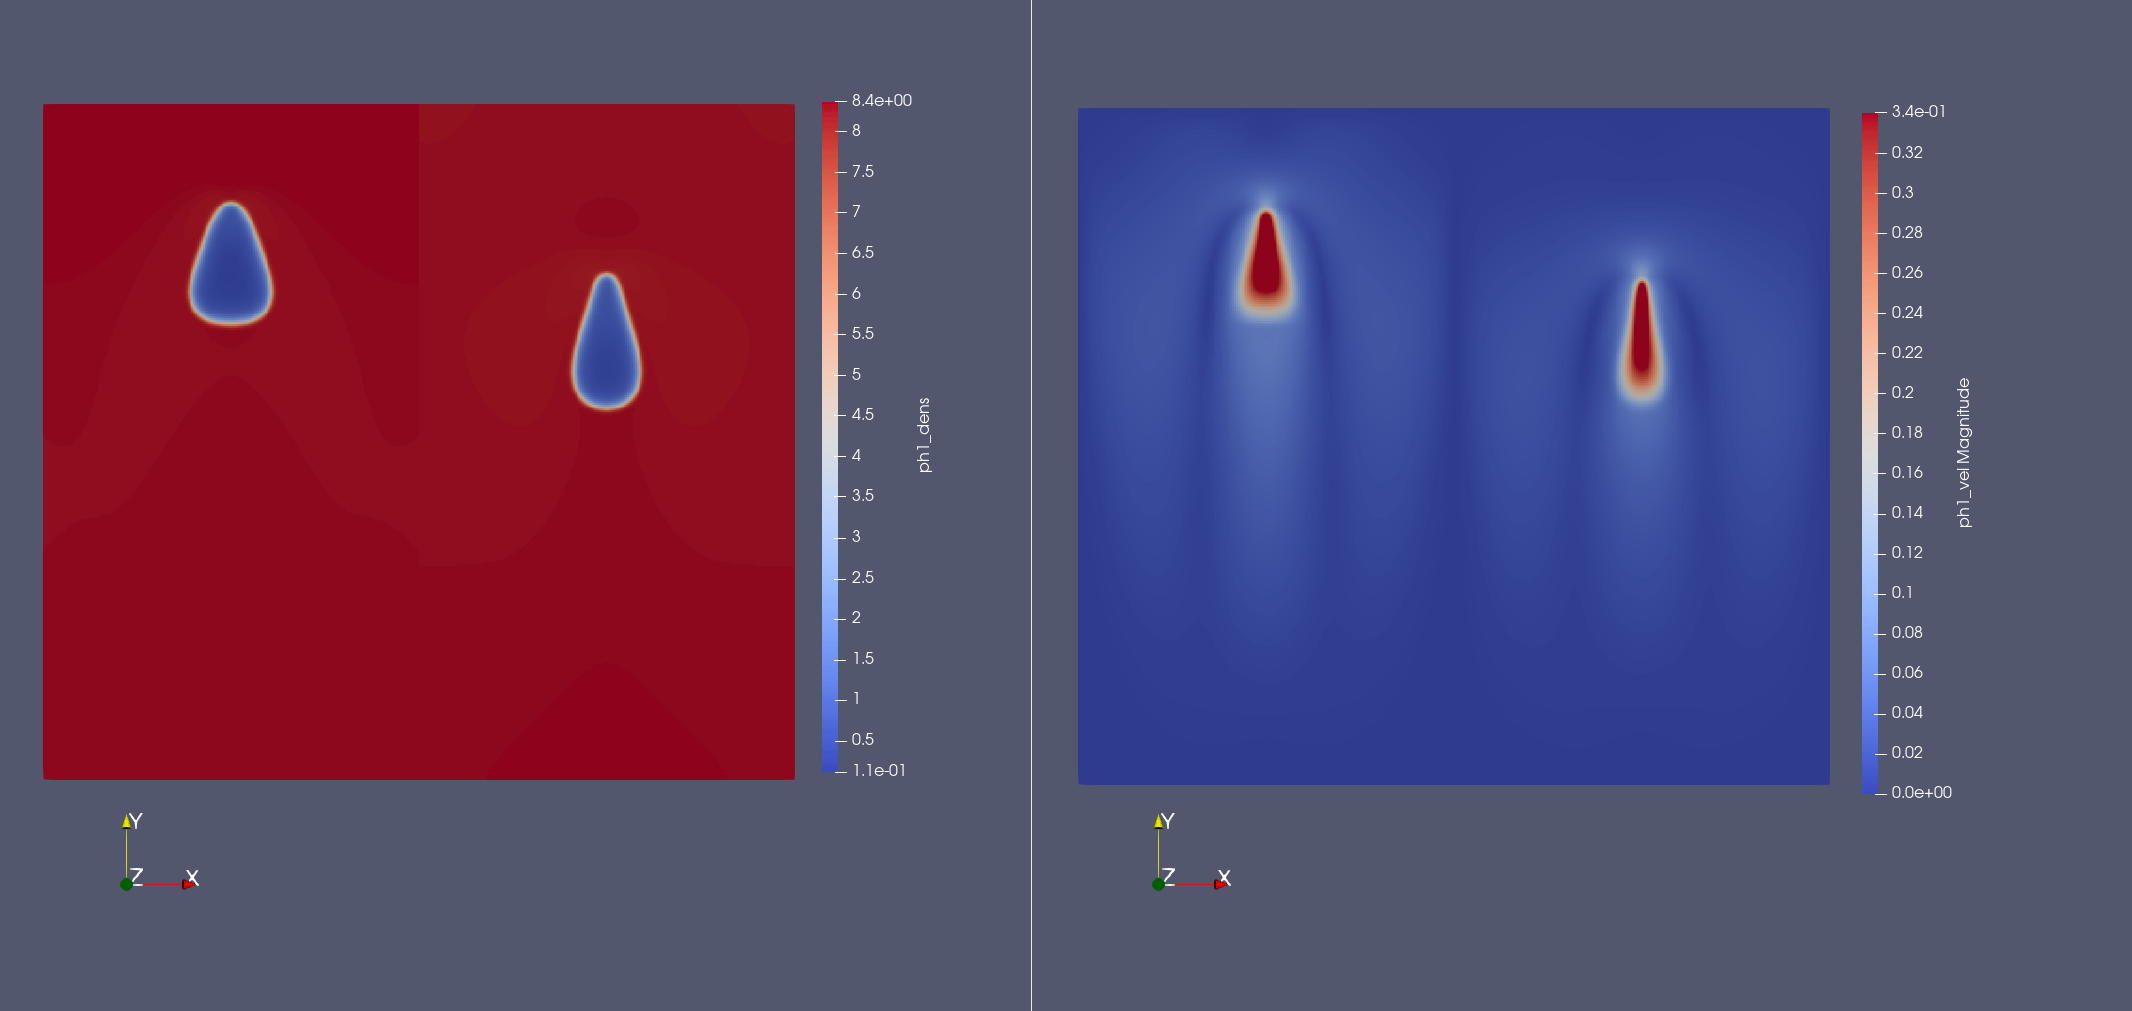
\includegraphics[scale=0.15]{pics/risingMCComp.png}
			\\{\tiny \justifying Density and Velocity field}
		\end{figure}
	\end{frame}

	\begin{frame}{Difficulties in single phase}
		\textbf{}\\~\\
		\begin{itemize}
			\item Same as in single component
			\item Reach stable simulations
			\item Seems that walls are affecting more the shape than in the single component
		\end{itemize}
	\end{frame}

	\begin{frame}{Actions}
		\begin{columns}[T]
			
			\column{0.5\textwidth}
			Possible actions: Immiscible force. Implement periodic BCs with solid nodes in the boundary. ~\\
			
			Proposed by the group:
			\begin{itemize}
				\item Switch to periodic boundaries
				\item Use Shan-Chen to reproduce other's results
				\item Apply well-balanced model with Shan-Chen
				\item Look for $C_D$ for cylinders, as this is Stokes flow, and its truncation has an impact
				\item Reduce $d$, increase $g$. 
				
			\end{itemize}
			
			\column{0.5\textwidth}
			
		\end{columns}
	\end{frame}

	%---------------------------------------------------------
	%---------------------------------------------------------
	\subsection{Dr. Mehmani RG - LBM - Apr 28 - 2022}
	\label{}
	\justifying
	\begin{frame}{Dr. Mehmani RG - LBM - Apr 28 - 2022}
		\textbf{Lattice Boltzmann Method - Formulation and Current Research}
		
		~\\Outline:
		\begin{itemize}
			\item Motivation
			\item The Lattice Boltzmann Method - Formulation
			\item Dynamic validations
			\item Ongoing work
		\end{itemize}
	\end{frame}
	
	\begin{frame}{Motivation}
		
		Applications: 
		\begin{itemize}
			\item CO$_2$ mineralization, gas densification, and gas diffusion 
			\item Solute transport and phase distribution
			\item Relative permeabilities - wettability
		\end{itemize}
		
		~\\\textbf{Why a new code?}: 
		\begin{itemize}
			\item 3D version for arbitrary domains, forces, and boundary conditions
			\item Future parallelization
			\item Coupling with other transport equations
		\end{itemize}
		
		~\\~\\Fortran 90, Object Oriented, LBM code for multi-component ($N_c$) mixtures. Output in VTK format.
	\end{frame}


	\begin{frame}[t]
		\frametitle{The Lattice Boltzmann Method - Formulation}
		
		The Lattice Boltzmann Method is based on kinetic theory, that states:
		
		\begin{equation}\label{eq:LBPDE}
			\underbrace{\frac{\partial f_i(x,t)}{\partial t} + \mathbf{c}_i \frac{\partial f_i(x,t)}{\partial x}}_{\text{Streaming - DF Advection}} = \underbrace{\mathbf{\Omega}}_{\text{Collision}} 
		\end{equation}
		
		What in its discretized form\footnote{Going from \ref{eq:LBPDE} to \ref{eq:LBE}, what about spatial derivative?} becomes:
		\begin{equation}\label{eq:LBE}
			f_i(x+ \mathbf{c}_i \Delta t, t+\Delta t) - f_i(x, t) = - \mathbf{M}^{-1} \mathbf{S} [\mathbf{m}(x,t) - \mathbf{m}^{\text{eq}}]  + \hat{F}_i
		\end{equation}
		where $\mathbf{m}$ are vectors of moments, $\mathbf{S}$ is a relaxation diagonal matrix, and $\mathbf{M}$ is a fixed matrix depending on DnQm. $ \mathbf{m}^{\text{eq}} = f(f_i^{\text{eq}}, \mathbf{F})$.
	\end{frame}
	
	
	\begin{frame}
		\frametitle{Macroscopic variables}
		Density and velocity are computed as follows:
		\begin{equation}
			\rho = \sum_i f_i \, \, \, \, \, \, \, \,  \mathbf{u} = \sum_i \mathbf{c}_i f_i
		\end{equation}
		Two important constitutive equations:
		\begin{equation*}
			f_i^{\text{eq}} = \rho \omega_i \left[ 1 + \frac{\vec{u}\cdot \vec{\mathbf{c}_i}}{c^2_s} + \frac{(\vec{u}\cdot \vec{\mathbf{c}_i})^2}{2c^4_s}-  \frac{\vec{u}\cdot \vec{u}}{2c^2_s} \right]
		\end{equation*}
		
		\begin{equation*}
			\hat{F}_i = \frac{\mathbf{F}}{\rho} \frac{\vec{u} - \vec{\mathbf{c}_i}}{c^2_s} f_i^{\text{eq}}  
		\end{equation*}
		
		where $\mathbf{F}$ is defined in the multiphase problem, as the Shan Cheng force:
		\begin{equation}
			\mathbf{F} = -G \psi(x) \sum_i \omega_i \psi(x+\mathbf{c}_i \delta t) \mathbf{c}_i \, \, \, \, \, \psi := \sqrt{\frac{2(P^{\text{\tiny EoS}}-c_s^2\rho)}{G \delta t c_s^2}}
		\end{equation}
	\end{frame}
	
	\begin{frame}{Dynamic Validations}
		
		The main validation sources are: analytical solutions, Cheng's codes, qualitative physics understanding.\\~\\
		
		
		\begin{columns}[T]
			
			\column{0.5\textwidth}
			Single phase:
			\begin{itemize}
				\item Channel flow ($\mathbf{F}$ \& $\nabla p$-driven)
				\item Couette flow (plates)
				\item Cylinder (turbulent)
				\item Cavity flow
				\item Porous medium
			\end{itemize}
			
			\column{0.5\textwidth}
			Multiphase:
			\begin{itemize}
				\item Static droplet
				\item Oscillation droplet
				\item Falling droplet
			\end{itemize}
		\end{columns}
	\end{frame}
	
	\begin{frame}{Single phase validations (quantitative)}
		\begin{figure}[h]
			\centering
			\begin{subfigure}{.5\textwidth}
				\centering
				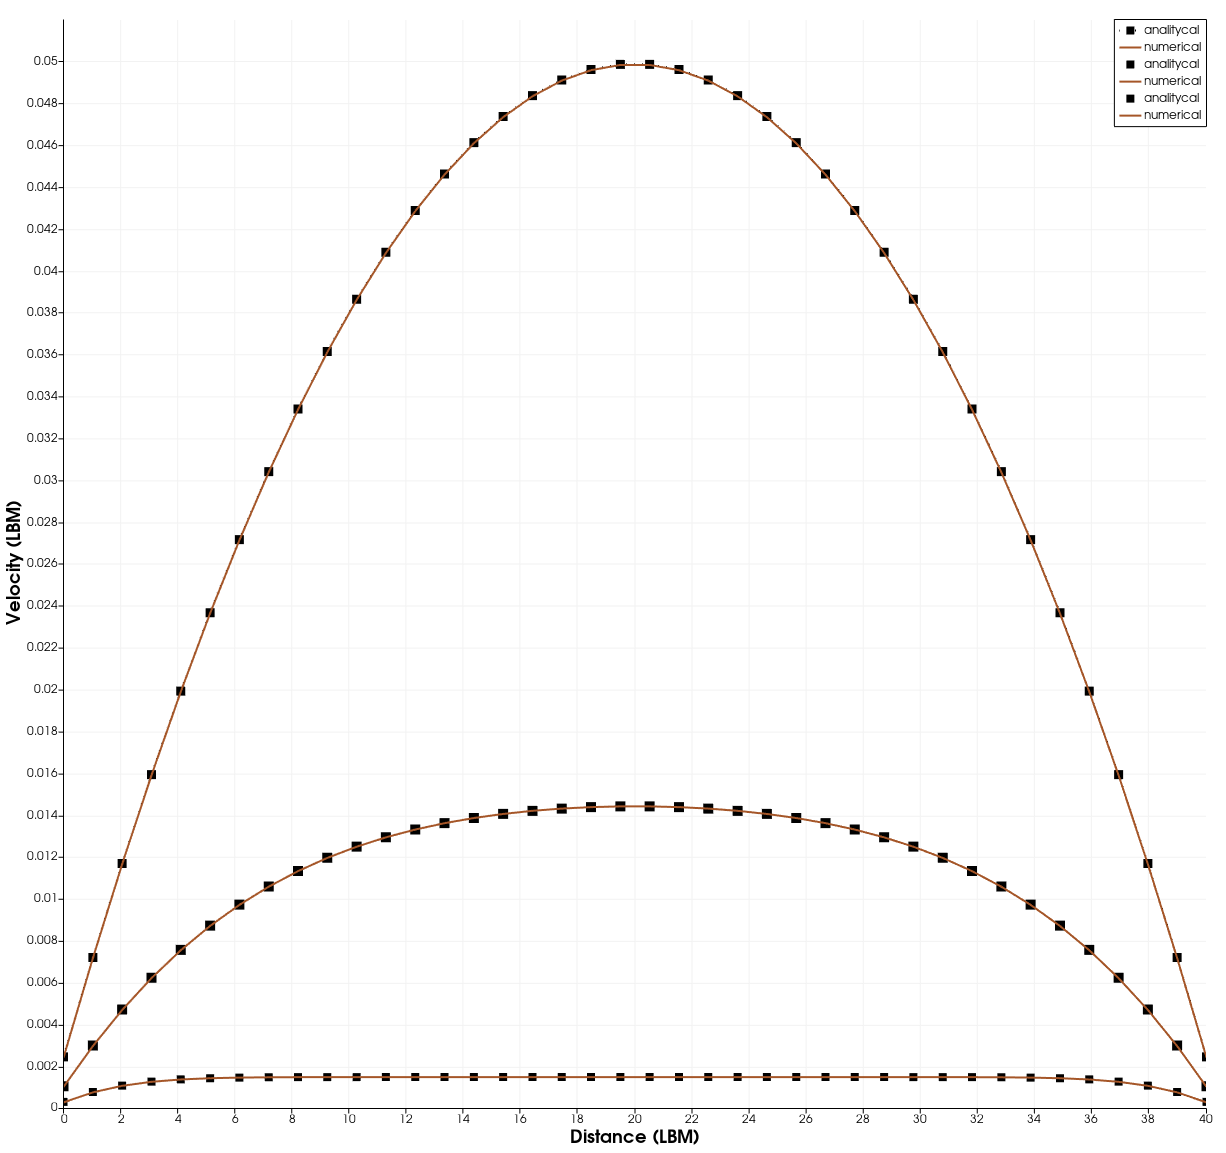
\includegraphics[width=.9\linewidth]{pics/channelForceDrivenValidation.png}
				\caption{$\mathbf{F}$-driven channel flow}
				\label{fig:sub1}
			\end{subfigure}%
			\begin{subfigure}{.5\textwidth}
				\centering
				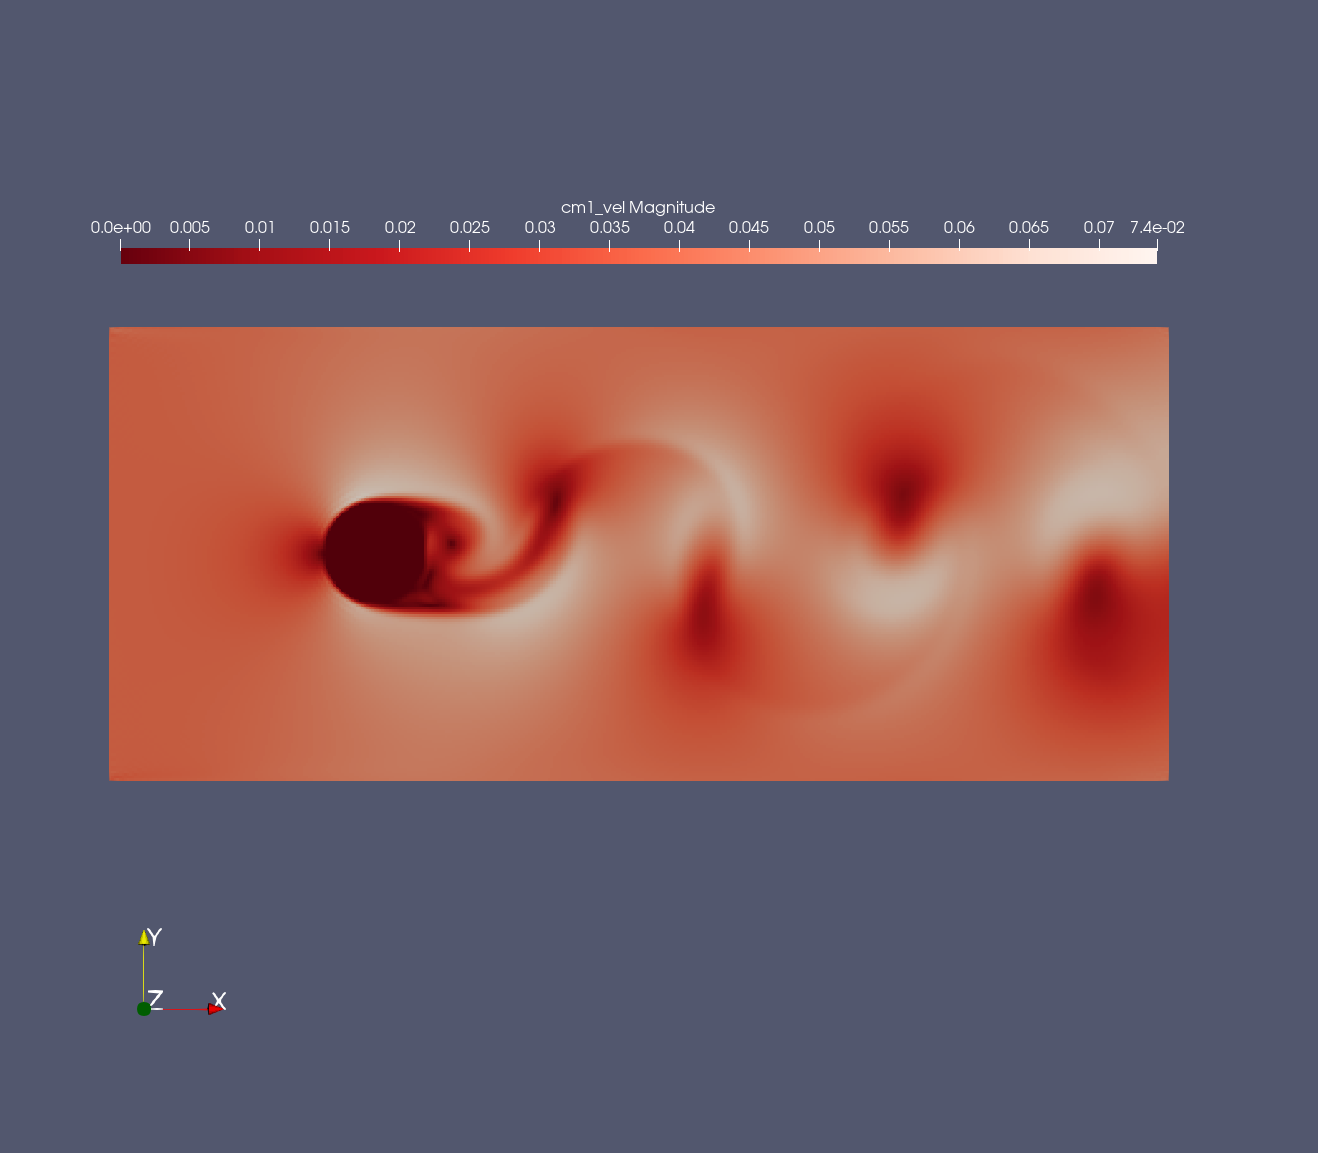
\includegraphics[width=.9\linewidth]{pics/cylinderTurbulent.png}
				\caption{Turbulent flow around cylinder}
				\label{fig:sub2}
			\end{subfigure}
			\caption{Results with direct source for quantitative comparisons.}
			\label{fig:osci}
		\end{figure}
	\end{frame}
	
	\begin{frame}{Single phase validations (qualitative)}
		\begin{figure}[h]
			\centering
			\begin{subfigure}{.5\textwidth}
				\centering
				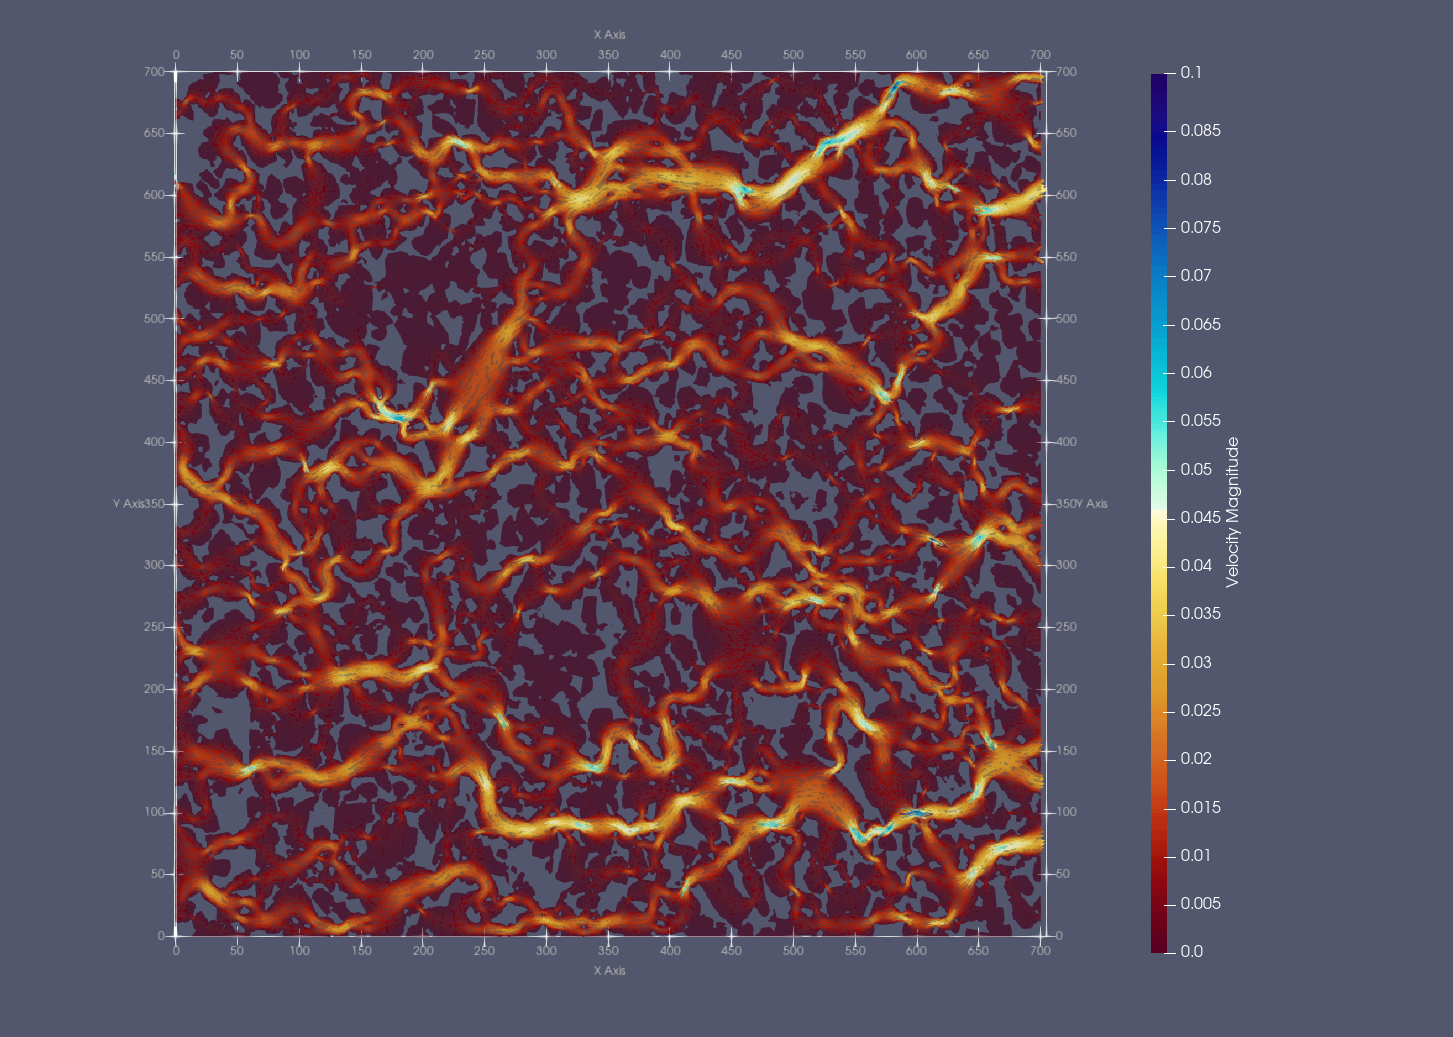
\includegraphics[width=.9\linewidth]{pics/pmVelLowV.png}
				\caption{Arbitrary porous medium (real image).}
		
			\end{subfigure}%
			\begin{subfigure}{.5\textwidth}
				\centering
				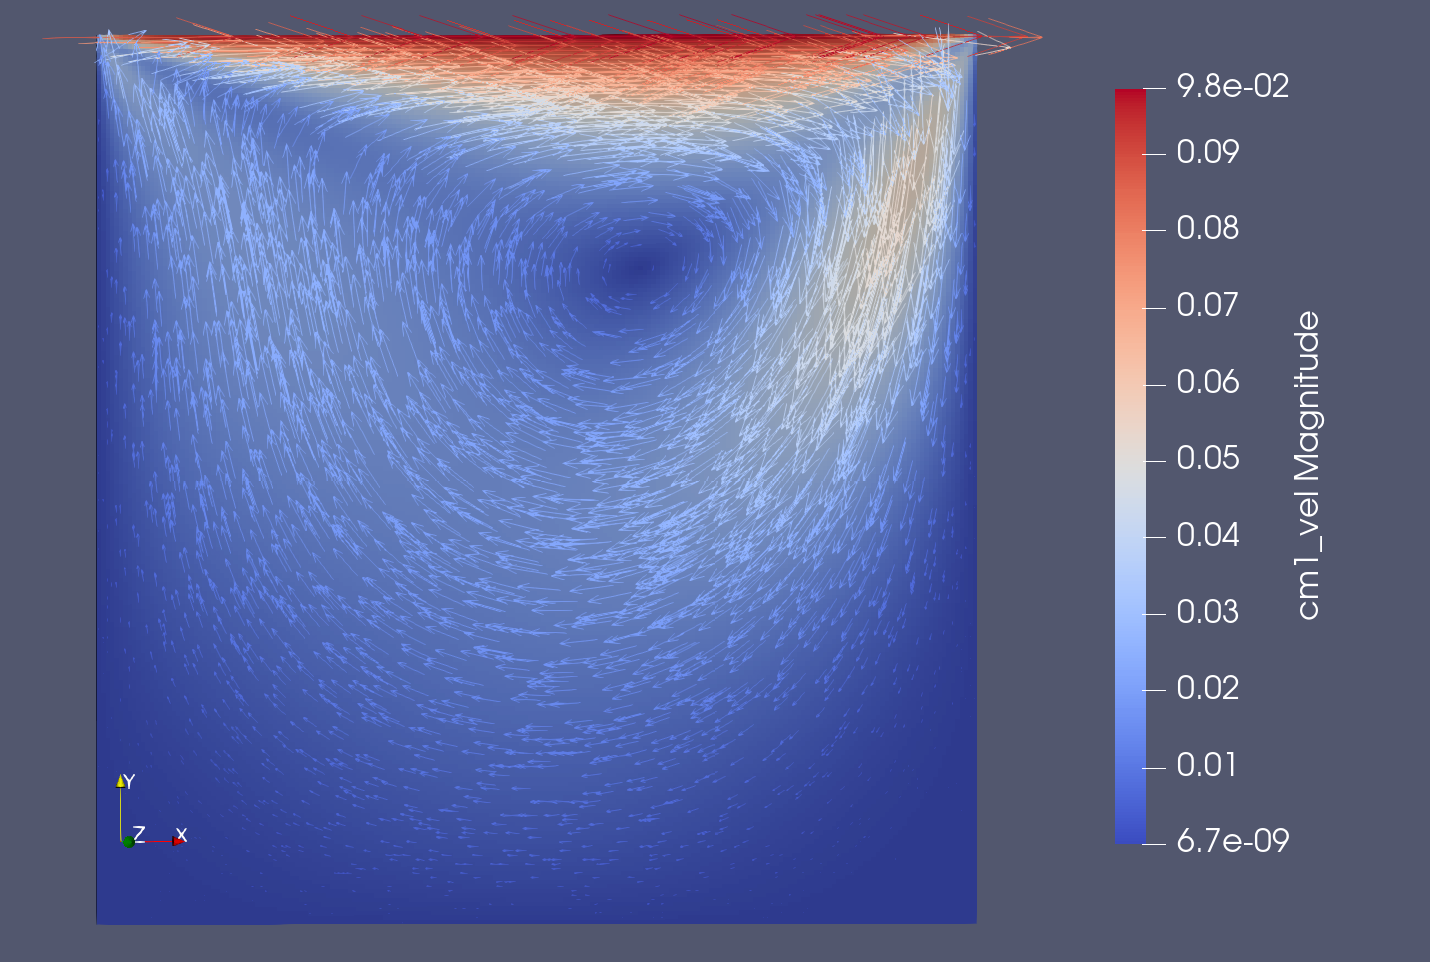
\includegraphics[width=.9\linewidth]{pics/cavity.png}
				\caption{Cavity flow, imposing a velocity on the upper wall.}
		
			\end{subfigure}
			\caption{Single phase cases qualitatively demonstrating the ability of modeling arbitrary porous media and arbitrary boundary conditions.}
	
		\end{figure}
	\end{frame}
	
	\begin{frame}{Multiphase single component - Oscillating droplet}
		\begin{figure}[h]
			\centering
			\begin{subfigure}{.5\textwidth}
				\centering
				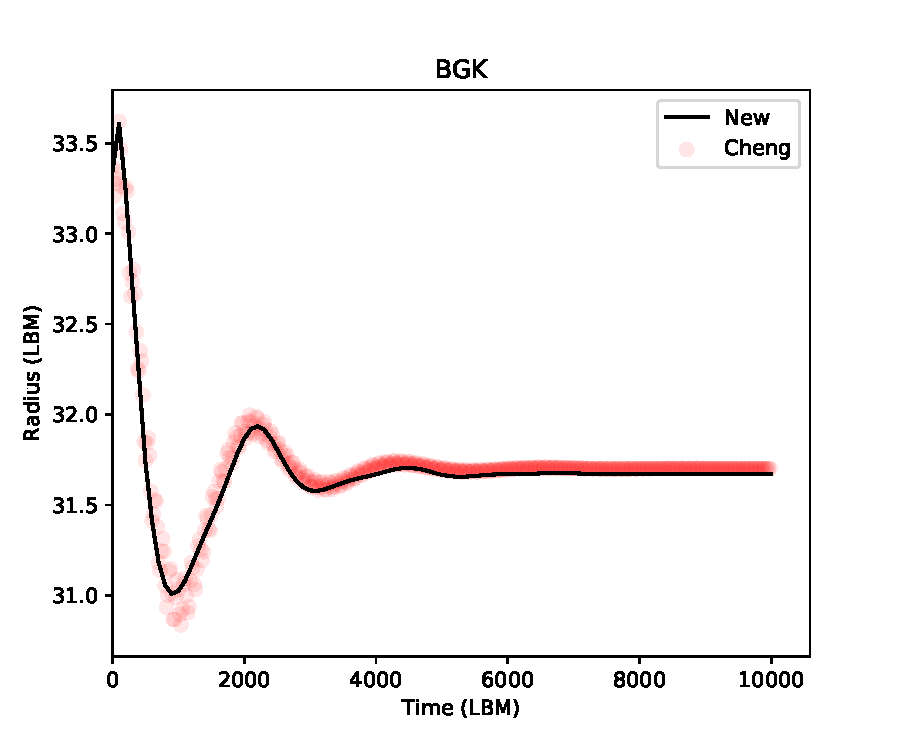
\includegraphics[width=.9\linewidth]{pics/BGKOsc.pdf}
				\caption{BGK}
	
			\end{subfigure}%
			\begin{subfigure}{.5\textwidth}
				\centering
				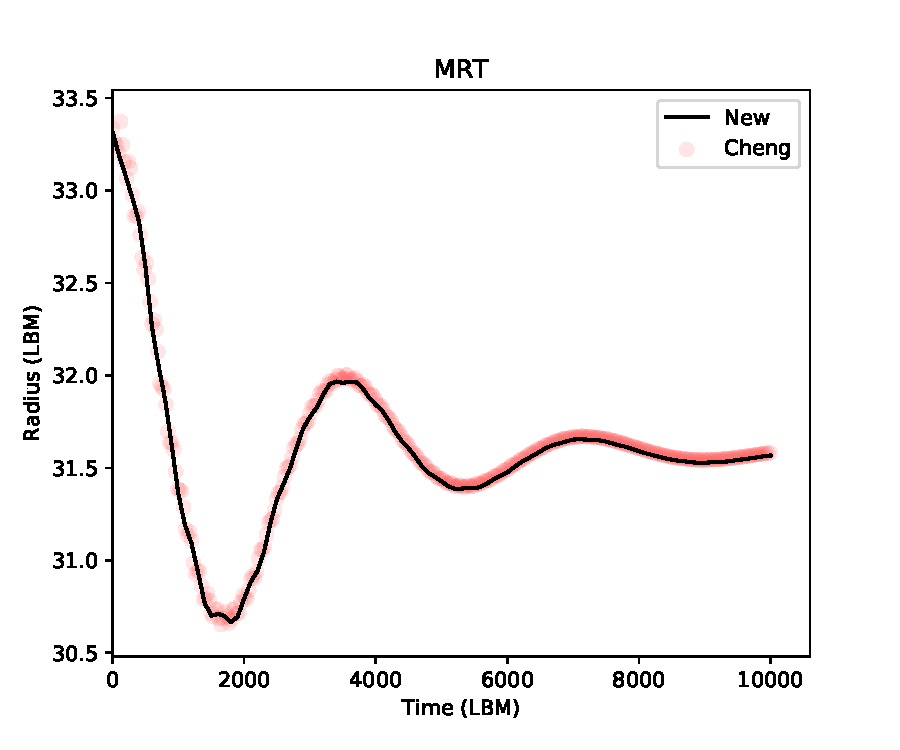
\includegraphics[width=.9\linewidth]{pics/MRTOsc.pdf}
				\caption{MRT}

			\end{subfigure}
			\caption{Oscillation droplet case. Viscosities are different in each case.}
		\end{figure}
	\end{frame}
	
	
		\begin{frame}{Static results - Young Laplace}
		$P_c = \frac{\sigma}{r}$, for a 2D geometry.
		$\sigma = $ 0.12141. Here, $r = R_e$, the equilibrium radius.
		
		\begin{figure}[h]
			\centering
			\begin{subfigure}{.5\textwidth}
				\centering
				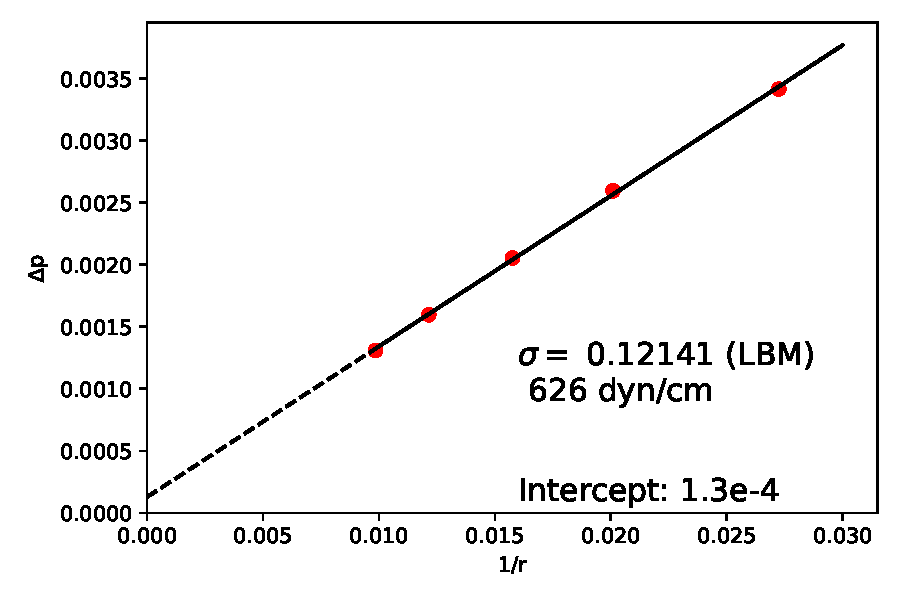
\includegraphics[width=1\linewidth]{pics/IFT.pdf}
				\caption{Young-Laplace validation}
			\end{subfigure}%
			\begin{subfigure}{.5\textwidth}
				\centering
				\includegraphics[width=1\linewidth]{pics/2c_staticRChange.png}
				\caption{Evolution of $R_e$ for the static cases.}
			\end{subfigure}
			\caption{Young Laplace and $R_e$ change due to thermodynamic inconsistency.}
			\label{fig:laplace}
		\end{figure}
		
	\end{frame}
	
	\begin{frame}{Oscillating droplet}
		$R_{x,0} = 60, R_{y,0} = 0.9 R_{x,0}$, in a grid of 400x400. $\tau_l = \tau_v = 0.56$, to reduce the viscous dissipation.
		\begin{figure}[h]
			\centering
			\includegraphics[scale=0.4]{pics/2cOsc.pdf}
			\caption{Oscillation of the X axis compared with Cheng's solution.}
			\label{fig:2cOsc}
		\end{figure}
	\end{frame}
	
	\begin{frame}{Fourier transform}
		
		\begin{columns}
			
			\column{0.5\textwidth}
			\begin{figure}[h]
				\centering
				\includegraphics[width=1\linewidth]{pics/fourier.pdf}
				\caption{Maximum amplitude at $T_n = 10010$.}
				\label{fig:2cOsc}
			\end{figure}
			
			\column{0.5\textwidth}
			Analytical solution:
			\begin{equation}
				T_a = 2 \pi \left[ \frac{n (n^2-1) \sigma}{\rho_l R_e^3} \right]^{-0.5}
			\end{equation}
			Giving a period $T_a = $ 9989. This gives a relative error of 2\%. 
		\end{columns}	
	\end{frame}
	
	\begin{frame}{Ongoing work - Raising bubble physics}
		
		\begin{columns}[T]
			
			\column{0.5\textwidth}
			
			\begin{itemize}
				\item Main properties
				\begin{itemize}
					\item Surface tension
					\item Body forces
					\item Viscosity and density ratio
					\item Boundary conditions
				\end{itemize}
				
				\item Bond and Morton numbers fix $R_e = \frac{u_t d_b}{\nu_l}$
				\begin{equation*}
					\begin{split}
						B_o = \frac{g \Delta \rho d_b^2}{\sigma}\\
						M_o = \frac{g \Delta \rho \mu_l^4}{\sigma^3 
							\rho_l^2}
					\end{split}
				\end{equation*}
				
				\item The drag coefficient, $C_D$, function of $R_e$, and defined as: 
				\begin{equation*}
					\begin{split}
						C_D = \frac{4 \Delta \rho g d_b}{3 u_t^2 \rho_l}
					\end{split}
				\end{equation*}
				resulting from a drag and gravity force balance. 
			\end{itemize}
			
			\column{0.5\textwidth}
			\begin{figure}
				\centering
				\includegraphics[scale=0.2]{pics/shapeRegimes.png}
				\\{\tiny \justifying Taken from Amaya-Bower L., Lee T. Single bubble rising dynamics for moderate Reynolds number using Lattice Boltzmann Method. Computer and Fluids. 2010.}
			\end{figure}
			
		\end{columns}
		
	\end{frame}
	
	\begin{frame}{Experimental relationship of $C_D$ with $R_e$}
		
		The constants may change due to the 2D approximation. 
		\begin{figure}
			\centering
			\includegraphics[scale=0.2]{pics/dragRe.png}
			\\{\tiny \justifying Taken from API Specifications for Oil and Gas Separators and PNG 480 Handout. L. Ayala, H. Emami-M. }
		\end{figure}
	\end{frame}
	
	\begin{frame}[t]{Considerations}
		\justifying
		
		\begin{columns}[T]
			
			\column{0.45\textwidth}
			\textbf{Goal}~\\
			\justifying
			
			Test the pseudopotential approach for partially misc. mixtures, under the action of gravity.\\~\\
			
			\textbf{Methodology}~\\
			Test different flow regimes based on Bond (Eotvos) and Morton numbers. Validate against \textbf{terminal velocities and bubble shapes.}
			
			\begin{equation*}
				R_e = \frac{\rho_l u_b d_b}{\mu_l}
			\end{equation*}
			\begin{equation*}
				B_o = \frac{g \Delta \rho d_b^2}{\sigma} \,\,\,\, 	M_o = \frac{g \Delta \rho \mu_l^4}{\sigma^3 
					\rho_l^2}
			\end{equation*}
			
			
			A thermodynamic state fixes $\rho, \Delta \rho, \sigma$. At a given temperature, in a single component case, some values are provided ($\rho, \Delta \rho$) and others can be obtained by simulating the static droplet ($\sigma$). \\
			
			\column{0.45\textwidth}{
				\justifying
				
			}
			
			\textbf{Procedure}	
			\begin{itemize}
				\item Select $B_o$
				\item Calculate the gravity $g = \frac{B_o \sigma}{\Delta \rho d_b^2}$
				\item Select $M_o$
				\item Calculate $\mu_l^4 = \frac{M_o \sigma^3 \rho_l^2}{g \Delta \rho }$
				\item Select the viscosity ratio
				\item Calculate $\mu_g = \mu_l * \frac{\mu_g}{\mu_l}$
			\end{itemize}
			
			The LBM parameters are thus fixed:
			
			\begin{equation*}
				\begin{split}
					\tau = \frac{\nu}{c_s^2}+ \frac{\Delta t}{2}
				\end{split}
			\end{equation*}
			
			\textbf{Try single component and then the multicomponent case.}
		\end{columns}
	\end{frame}
	
	\begin{frame}[t]{Simulation setup (Amaya)}
		\justifying
		\begin{columns}[t]
			\column{0.45\textwidth}
			
			\textbf{Domain}: (!) 200x360 mesh (2D)\\
			\textbf{Fluid}: Water at 485.33 K ($T_r$ = 0.75), and $P_r$ = 0.092. \\$\rho_l^0$  = 7.679 (), $\rho_v^0$  = 0.109. $\rho_L/\rho_g$ = 70. $\tau_l$ = 210.5. $\tau_g$ = 0.8. $\mu_l/\mu_g$ =10.\\~\\
			Initial condition: Spherical droplet with $d_o$ = 40, and $w_o$ = 8.
			
			~\\
			\textbf{Boundary conditions}: No-slip condition on all boundaries.
			
			~\\
			\textbf{Parameters}: Shan-Chen $G$=-1.0. \\
			Beta = 0.9\\
			Time = 10000 ($\approx 10 \sqrt{\frac{d_b}{g}}$)\\
			~\\
			
			
			
			\column{0.45\textwidth}
			
			
			\textbf{Single static simulation}:\\ $\Delta \rho $ = 7.2 (7.7-0.5), $d_s$ = 40.0, \\ $\Delta P$ = 8.5e-3 - 5.87e-3 = 2.623e-3 \\$\sigma = \Delta P \cdot r$ = 0.05254.\\
			
			
			First, the single component case was tested as follows:
			\begin{enumerate}
				\item $B_o$ = 1. $M_o$ = 3e-5. $\mu_R$ = 100. 
				\item $B_o$ = 10. $M_o$ = 2e-2. $\mu_R$ = 10.
				\item $B_o$ = 10. $M_o$ = 2e-2. $\mu_R$ = 100. 
				\item $B_o$ = 0.1. $M_o$ = 1e-2. $\mu_R$ = 100.
				\item $B_o$ = 22. $M_o$ = 8.4e-4. $\mu_R$ = 100. 
			\end{enumerate}
		\end{columns}
	\end{frame}
	
	\begin{frame}{Preliminary Results}
		\begin{figure}
			\centering
			\includegraphics[scale=0.2]{pics/risingCompDen.png}
			\\{\tiny \justifying Bubble shapes}
		\end{figure}
	\end{frame}
	
	\begin{frame}{Preliminary Results}
		\begin{figure}
			\centering
			\includegraphics[scale=0.2]{pics/risingCompVel.png}
			\\{\tiny \justifying Velocity field}
		\end{figure}
	\end{frame}
	
	\begin{frame}{Difficulties in single phase}
		\textbf{}\\~\\
		\begin{itemize}
			\item Reach low Morton values (due to restrictions in kinematic viscosity).
			\item Reach high Bond numbers (high gravity)
			\item The cap shapes are not being observed, and the ellipsoidal tends to be more triangular.
			\item Hard to change Bond with fixed $\sigma$. System becomes unstable with other values of $G$.
		\end{itemize}
	\end{frame}
	
	
	\begin{frame}{Increasing the Morton number}
		Trying to make the liquid more viscous (at $B_o$ = 10), seems to not allow the bubble to rise ($M_o$ = 8e6), which later collapses.\\~\\
		\begin{itemize}
			\item $\tau_g$ = 0.52. $\tau_l$ = 47
			\item $\tau_g$ = 2.0. $\tau_l$ = 47 
			\item $\tau_g$ = 0.92. $\tau_l$ = 4.7 
		\end{itemize}
		\begin{figure}
			\centering
			\includegraphics[scale=0.15]{pics/risingCompDen456.png}
			\\{\tiny \justifying Velocity field}
		\end{figure}
	\end{frame}
	
	\begin{frame}{Potential solutions}
		\textbf{}\\~\\
		\begin{itemize}
			\item Fix MRT parameters
			\item Consider an implicit scheme
			\item Compare against the usual Shan-Chen force which may provide better stability 
		\end{itemize}
	\end{frame}
	
	\begin{frame}{Multicomponent case - First approach}
		\textbf{MC case with the beta model}\\~\\
		Using the same mixture that was used for the oscillating droplet, with a viscosity ratio of 10, two cases were run:
		\begin{itemize}
			\item $B_o$ = 10, $M_o$ = 5e-3.
			\item $B_o$ = 10, $M_o$ = 5e-4.
		\end{itemize}
	\end{frame}
	\begin{frame}{Multicomponent case - First approach}
		\begin{figure}
			\centering
			\includegraphics[scale=0.15]{pics/risingMCComp.png}
			\\{\tiny \justifying Density and Velocity field}
		\end{figure}
	\end{frame}
	
	\begin{frame}{Difficulties in single phase}
		\textbf{}\\~\\
		\begin{itemize}
			\item Same as in single component
			\item Reach stable simulations
			\item Seems that walls are affecting more the shape than in the single component
		\end{itemize}
	\end{frame}
	
	\begin{frame}{}
		\centering
		Thank you!
	\end{frame}


	%---------------------------------------------------------
	%---------------------------------------------------------
	\subsection{LBM Meeting - June 10 - 2022}
	\label{}
	\justifying
	\begin{frame}{LBM Meeting}
		\textbf{June 10 - 2022}\\~\\
		Recap from last meeting (see \ref{meet:LBM00422}):
		\begin{itemize}
			\item The splitting coef. did not provide stable simulations for a rising bubble. Possible reasons:
				\begin{itemize}
					\item Interaction with walls in closed domain
					\item Incorrect initial conditions
				\end{itemize}
			\item Main task from last meeting: reproduce bubbly flow with simpler model and compare
			\item The paper aims to test the scheme under dynamic conditions
		\end{itemize}
		
		~\\Today:
		\begin{itemize}
			\item Sankaranarayanan (Sankarana) scheme and rising bubble revisited
			\item Comparison with splitting coefficient
			\item New force scheme with no splitting coefficient
			\item Next direction
		\end{itemize}
	\end{frame}


	
	\begin{frame}[t]{Sankaranarayanan}
		In literature, many articles refer to this model to simulate bubbly flow with LBM. The model uses two components with a force defined by:
		
		\begin{equation}
			F_i^\sigma = - \psi^\sigma(\locx) \sum_{\sigma_2} G_{\sigma,\sigma_2} \sum_\alpha \psi^{\sigma_2} ( \locx + \vele \delta t)  w_\alpha \vele
		\end{equation}
		where:
		\begin{equation*}
			\psi^{(1)} (\rho) = \rho, \, \, \,  \psi^{(2)} (\rho) = \sqrt{\frac{\rho}{1-b\rho} - a \rho^2 - \rho}
		\end{equation*}
		
		The authors claim second component follows a van der Waals-type EoS, while the first one an ideal gas law. Such model produces the pressure equation:

		\begin{equation}
			\label{eq:pressureLBMPseudoP}
			\begin{split}
			p = c_s^2 \rho + \frac{c_s^2 \delta t}{2} \sum_\sigma \sum_{\sigma_2} G_{\sigma,\sigma_2} \psi_\sigma \psi_{\sigma_2} 
			\end{split}
		\end{equation}
		In the model, the interaction parameters can represent either attraction or repulsion.
		
		\begin{alertblock}{Important remark}
			This scheme is not thermodynamic consistent, but was able to represent \textbf{hydrodynamics} and forces pointing to \textbf{opposite directions}.
		\end{alertblock}
	\end{frame}

	\begin{frame}{Simulation setup}
		\justifying
		\begin{columns}[t]
			\column{0.45\textwidth}
			
			\textbf{Domain}: 160x400 mesh (2D)\\

			\textbf{Fluid}:
			\begin{tabular}{|c|c|c|c|c|}
				\hline
				Name & $\omega$ & Tc & Pc & Mw \\
				\hline
				C3 & 0.152 & 370 & 42.46 & 0.0441 \\
				\hline
				C5 & 0.251 & 470 & 33.68 & 0.0722 \\
				\hline
			\end{tabular}
		
			Temperature = 306.7 K (Tr = 0.83). \\
			
			Equilibrium conditions \\(equimolar, 60 psi): \\
			$\rho_l, \rho_v$ (lbm/ft3) = 37.5, 0.54. \\
			$mw_l, mw_v$ (g/mol) = 62.8, 48.9. \\
			$\bar{\rho}_\text{ratio}$ = 14.3.\\ 
			$K_1, K_2$ = 2.49, 0.25. $\gamma$ = 0.5744. \\~\\
			\textbf{Boundary conditions}: Full periodic.
			\textbf{Initial conditions}: Bubble in equilibrium, $r_0, w_0$ = 24, 5 lu.
			
			
			\column{0.45\textwidth}
			Each model requires a different initialization (close to its equilibrium) ~\\
			(otherwise, spinodal decomposition appears).\\~\\
			
			\textbf{Parameters}:\\
			Sankarana: Attraction and repulsion G: $G_{11}=0, G_{12}=1, G_{22}=-1$\\
			$\beta$ = 1.0 (prevent further decomposition)\\
			Time = 1e4 (static), 1e5 (dynamic)\\
			
			\begin{equation*}
				\begin{split}
				B_o = \frac{g \Delta \rho d_b^2}{\sigma}\\
				M_o = \frac{g \Delta \rho \mu_l^4}{\sigma^3 \rho_l^2} = \frac{g \Delta \rho \nu_l^4 \rho_l^2}{\sigma^3}\\
				\nu_v = \nu_l \cdot \underbrace{\frac{\mu_v}{\mu_l}}_{\mu \text{ ratio inv.}} \cdot \frac{\rho_l}{\rho_v}
				\end{split}
			\end{equation*}
			
		\end{columns}
	\end{frame}

	\begin{frame}[t]{Static Results}

		\begin{columns}[t]
			\column{0.45\textwidth}
			Sankarana:\\~\\
			Initialization: $\rho_l$ = 5.75, $\rho_v$ = 2.17. ~\\
			$x_{1,l}$ = 0.02, $x_{1,v}$ = 0.52. ~\\

			Static results:\\
			$\rho_l$ = 5.77, $\rho_v$ = 2.17. $x_{1,l}$ = 0.02, $x_{1,v}$ = 0.47. For $r_e$ = 27, $\Delta p = \frac{\sigma}{r}$ = 0.00274. $\sigma$ = 0.074.
			\begin{equation*}
				\begin{split}
				B_o = 141 465 \cdot g \, \, \, \, \, M_o = 294 952 \cdot g \cdot \nu^4_l\\
				\nu_v = 0.02645 \nu_l 
				\end{split}
			\end{equation*}

			\column{0.45\textwidth}
			Splitting Coefficient Scheme:\\~\\
			Initialization: $\rho_l$ = 8.069, $\rho_v$ = 0.1157. ~\\
			$x_{1,l}$ = 0.234, $x_{1,v}$ = 0.750. ~\\

			Static results:\\
			$\rho_l$ = 8.07, $\rho_v$ = 0.358. $x_{1,l}$ = 0.234, $x_{1,v}$ = 0.58. For $r_e$ = 25.1, $\Delta p = \frac{\sigma}{r}$ = 0.00285. $\sigma$ = 0.072.
			\begin{equation*}
				\begin{split}
				B_o = 67 481 \cdot g \, \, \, \, \, M_o = 6976 \cdot g \cdot \nu^4_l\\
				\nu_v = 0.2254 \nu_l
				\end{split}
			\end{equation*}

		\end{columns}

		\begin{figure}
			\centering
			\includegraphics[scale=0.15]{pics/shapeRegimes.png}
		\end{figure}

	\end{frame}

	\begin{frame}[t]{Dynamic results with Sankarana}
		\begin{columns}
			\column{0.25\textwidth}
			Spherical:
			\begin{figure}
				\centering
				\includegraphics[width=1.0\textwidth]{pics/bubbles/spherical1st.png}
			\end{figure}
			
			\column{0.25\textwidth}
			Ellipsoidal
			\begin{figure}
				\centering
				\includegraphics[width=1.0\textwidth]{pics/bubbles/ellipsoidal1st.png}
			\end{figure}
		
			\column{0.25\textwidth}
			Cap:
			\begin{figure}
				\centering
				\includegraphics[width=1.0\textwidth]{pics/bubbles/dimple1st.png}
			\end{figure}
		\end{columns}
		
		~\\~\\Animations that provide further insight:
		\begin{itemize}
			\item Spinodal decomposition and rising (small square) (spinodalAndDimple.mp4)
			\item Rising in long channel (channelSankaraRissing.mp4)
			\item Bubbly flow under gravity (bubblyFlowSCIM.mp4)
			\item Spinodal decomposition and coalescence (coallescence.avi)
			\item Dependence on initial conditions (bubbleComparisonSankaInit and bubbleComparisonVWInit)
		\end{itemize}
	\end{frame}

	\begin{frame}{Direction of the cohesion force}
		\begin{figure}
			\includegraphics[width=\textheight]{pics/bubbles/forceProfileSankSplit.png}
		\end{figure}
	\end{frame}
	\begin{frame}{Dynamic results with splitting coefficient}
		\begin{figure}
			\centering
			\includegraphics[width=1.0\textwidth]{pics/bubbles/comparisonSphElp.png}
		\end{figure}
	\end{frame}

	\begin{frame}{Observations}

		\begin{columns}[t]
			\column{0.45\textwidth}
			About the Sankaranarayanan model:
			\begin{itemize}
				\item The model allows for counterflow of components (force in opposite directions)
				\item It adapts to the hydrodynamic conditions, depicting the correct shapes (see shape diagrams).
				\item The model is not thermodynamic consistent and makes no sense that every component obeys a different law (EoS).
				
			\end{itemize}

			\column{0.45\textwidth}
			About Splitting coefficient:
			\begin{itemize}
				\item Both components are forced to move in the same direction (no matter current conditions)
				\item Once phase pressure is reached, components are \textit{trapped} and can not diffuse 
				\item Interaction of splitting coefficient with external forces seems to violate hydrodynamics
				\item Unstable. This is fixed by $u^{mod}_i = u_i + \frac{\beta F_i}{\tau - 0.5}$, but fugacities start to deviate.
			\end{itemize}
		\end{columns}
		~\\~\\
		\begin{itemize}
			\item About boundary conditions: reference density has to be constantly corrected, or velocity reset is required
			\item About numerical stability: how to reduce $\delta t$ without affecting the force magnitude (otherwise, density gradient is not supported)
		\end{itemize}
		
	\end{frame}

	\begin{frame}{Partial conclusions}
		\begin{itemize}
			\item The splitting coefficient requires a major revision for modeling rising bubbles 
			\item The Sankaranarayanan model should be used to extract qualitative features, and adapt those in a dynamic splitting coefficient
			\item For the paper purposes, a different scenario should be simulated:
			\begin{itemize}
				\item Droplet splash
				\item Rayleigh-Taylor instability  
			\end{itemize}
			\item Implement a free energy-based scheme (in any of its flavors) may elucidate in the correct splitting expression
			\item The work on rising bubble allowed to identify current limitations that can be later exploited 
		\end{itemize}
	\end{frame}

	\begin{frame}{New scheme based on the Sankarana ideas}

		Mass-basis cubic equation of state:
		\begin{equation*}
			p = \frac{R_sT}{(1-b_m \rho)} \rho - \frac{a_m \rho^2}{f(b_m \rho)} = c_s^2 \rho + \frac{c_s^2 \delta t}{2} \sum_\sigma \sum_{\sigma_2} G_{\sigma,\sigma_2} \psi_\sigma \psi_{\sigma_2} 
		\end{equation*}

		where the mixture parameters are defined as:
		\begin{equation*}
			a_m = \sum_\sigma \sum_{\sigma_2} \chi_\sigma \chi_{\sigma_2} \sqrt{a_\sigma a_{\sigma_2}} (1-\varLambda_{\sigma, \sigma_2}) \; \; \; \; \; a_m \rho^2 = \sum_\sigma \sum_{\sigma_2} \rho_\sigma  \rho_{\sigma_2} \sqrt{a_\sigma a_{\sigma_2}} (1-\varLambda_{\sigma, \sigma_2})
		\end{equation*}

		Finally, the pressure equation takes the convenient form:
		\begin{equation}
			p = \frac{R_sT}{(1-b_m \rho)} \rho - \sum_\sigma \sum_{\sigma_2} \rho_\sigma  \sqrt{\frac{a_\sigma}{f(b_m \rho)} } \rho_{\sigma_2} \sqrt{\frac{a_{\sigma_2}}{f(b_m \rho)} }   (1-\varLambda_{\sigma, \sigma_2})
		\end{equation}

		That resembles closely the pressure equation recovered with pseudo-potentials in the equation \ref{eq:pressureLBMPseudoP}.

		\begin{equation*}\label{eq:newPseudopotential}
			\psi(\rho_\sigma) = \rho_\sigma \sqrt{\frac{a_\sigma}{f(b_m \rho_m)}} \; \; \; \; b_m \rho_m = \sum_\sigma b_\sigma \rho_\sigma
		\end{equation*}
		
		and the interaction between components is exactly given by:
		\begin{equation*}
			G_{\sigma,\sigma_2} = \frac{2(\varLambda_{\sigma, \sigma_2}-1)}{c_s^2 \delta t} 
		\end{equation*}
	
	\end{frame}

	\begin{frame}{Final force expression}

		Force divided into two terms (attraction and repulsion): 
		
		\begin{equation}\begin{split}
			F_i^\sigma = - \psi^\sigma(\locx) \sum_{\sigma_2} G_{\sigma,\sigma_2} \sum_\alpha \psi^{\sigma_2} ( \locx + \vele \delta t)  w_\alpha \vele\\
			 - \frac{1}{c_s^2 \delta t} \sum_\alpha  w_\alpha \vele [\frac{R_sT}{1-b_m \rho} \rho_\sigma - c_s^2 \rho_\sigma ] ( \locx + \vele \delta t) 
		\end{split}
		\end{equation}
	\end{frame}
	

	\begin{frame}{Simulation setup}
		
		\begin{columns}
			
			\column{0.5\textwidth}
			From van der Waals implementation into the phase behavior model (C++):\\~\\
			
			Name, mw, pc, tc, acen, vc, shift\\
			C3 0.044097 615.8 666.05 0.1522 0.0 0.0\\
			C5 0.044097 488.5 845.80 0.2514 0.0 0.0\\~\\
			
			Conditions:\\
			P = 275.36 psi, T = 192.34 F. z = [0.5, 0.5]\\~\\
			
			Results from flash:
			
			Densities = 13.5852 lb/ft3, 2.3956 lb/ft3 (4.693187 lu, 0.8275917 lu)\\~\\
			Fugacities = 906.34 kPa, 604.423 kPa (0.043939432 lu, 0.029302344 lu)\\~\\
			Liquid composition = [0.36357, 0.63643]\\~\\
			Gas composition = [0.54527, 0.45473]\\~\\
			Ki = 1.49975, 0.714505. $\gamma$ = 0.642
			\column{0.5\textwidth}
			
		\end{columns}
		
	\end{frame}


	\begin{frame}{Results}
		The density profile converges to the correct values given by the vdW EoS. The splitting coefficient, with no calibration in $\beta$, compromises the vapor density to under predicted values.
		\begin{figure}
			\centering
			\includegraphics[width=\textwidth]{pics/1dnewForce/density.png}
		\end{figure}
	\end{frame}
	
	\begin{frame}{Results}
		The pressure with the new scheme converges to the correct pressure value. The splitting scheme, as the density of the vapor is lower, the convergence pressure is also lower. Due to the small compressibility of the liquid, to achieve this value of pressure, small changes in density are needed, so the liquid density is not compromised.
		\begin{figure}
			\centering
			\includegraphics[width=\textwidth]{pics/1dnewForce/pressure.png}
		\end{figure}
	\end{frame}

	\begin{frame}{Results}
		The compositions in both cases do not match with equilibrium values. This is due that the model does not allow for diffusion if the pressure is already in equilibrium. These results suggest that transport is favored to keep the liquid properties are they were initialized, and balances the vapor properties accordingly.
		\begin{figure}
			\centering
			\includegraphics[width=\textwidth]{pics/1dnewForce/massFraction.png}
		\end{figure}
	\end{frame}

	\begin{frame}{Results}
		Fugacities prove the non chemical-equilibrium in the system.
		\begin{figure}
			\centering
			\includegraphics[width=\textwidth]{pics/1dnewForce/fugacity.png}
		\end{figure}
	\end{frame}

	\begin{frame}{Results}
		\begin{figure}
			\centering
			\includegraphics[width=\textwidth]{pics/1dnewForce/forceX.png}
		\end{figure}
	\end{frame}
	
	\begin{frame}{Summary}
		General goal: Test the splitting coefficient scheme under dynamic conditions. \\
		
		What has been done so far:
		
		\begin{itemize}
			\item Implemented multicomponent LBM code for $n_c$ components and $n_f$ forces 
			\item Validated the implementation for single phase conditions (analytical solutions)
			\item Validated the splitting scheme in multiphase conditions: 
			\begin{itemize}
				\item Droplet oscillations
				\item \textbf{Rising bubble}
			\end{itemize}
		\end{itemize}
		
		Specific objectives:
		\begin{itemize}
			\item Writing the manuscript presenting the splitting scheme along with MRT 
			\item Present 2/3 dynamic scenarios 
			\item Find the conditions where the model is suitable
			\item Write the findings, and particularly, suitability and limitations
		\end{itemize}
		
		~\\
		Let's now analyze what was found for the rising bubble case.
	\end{frame}
	
	\begin{frame}{Actions to take}
		\begin{itemize}
			\item Design new simulation cases with no additional forces
			\item Write current findings (aiming to the paper)
			\item Start the free energy development
		\end{itemize}
	\end{frame}
	
	
	%---------------------------------------------------------
	%---------------------------------------------------------
	\subsection{Report - June 15 - 2022}
	\label{}
	\justifying
	\begin{frame}{}
		\textbf{June 15 - 2022}\\~\\
		Discussion topics:
		\begin{itemize}
			\item Free energy theory and implementation (see procedure)
			\begin{itemize}
				\item Mathematical procedure
				\item Questions about pressure tensor approach
				\item Thermodynamic properties as tensor quantities
			\end{itemize}
			\item Code sharing (and new branch for free energy)
			\begin{itemize}
				\item Code shared with Muzammil
				\item Code running in Windows (setup time: 1.5 h)
				\item Code efficiency: 3 times slower than Cheng's code, with no printing
				
			\end{itemize}
			\item Paper (update): splash case running
			\item Qualifying (update)
			\item Actions (to be defined)
		\end{itemize}
		
	\end{frame}
	
	\begin{frame}[t]{Free energy theory}
		Continuity and Navier-Stokes equation:
		\begin{equation*}
			\begin{split}
			\partial_t \rho + \partial_\alpha (\rho u_\alpha) = 0\\
			\rho \partial_t u_\alpha  + \rho u_\beta \partial_\beta (u_\alpha) = \partial_\beta \sigma_{\alpha\beta} + \rho f_\alpha +  \color{red} f^s_\alpha
			\end{split}
		\end{equation*}
		
	where the stress tensor is defined as:
	\begin{equation*}
			\sigma_{\alpha\beta} = -p \kronecker + \lambda \partial_\gamma u_\gamma \kronecker + \mu (\partial_\beta u_\alpha + \partial_\alpha u_\beta)
	\end{equation*}
	
	According with Currie's book \footnote{Fundamentals in Fluid Mechanics}, a mechanical pressure, "accounting only for the translational energy of the molecules", can be defined as $\bar{p} = \sum_\alpha \sigma_{\alpha\alpha} /3$. The thermodynamic pressure (which account for all energy modes, including intermolecular attraction) and the mechanical pressure are related by:
	\begin{equation*}
		p - \bar{p} = (\lambda + \frac{2}{3}) \nabla \cdot u = K  \partial_\gamma u_\gamma
	\end{equation*}
	
	However, this result does not account for the surface tension force $\color{red} f^s_\alpha$. It is probable then, that this relationship needs to be redefined. It is argued that $K=0$ for monoatomic gases, which do not have vibrational or rotational energy modes (although they do not claim that they still may have intermolecular attraction). In that case $\lambda = -\frac{2}{3}$, modifying the stress tensor. As this term did not arise in the CE expansion, should we include it in $\sigma_{\alpha\beta}$? The only case where both expressions converge, is where we have an incompressible fluid ($\nabla \cdot u = \partial_\gamma u_\gamma = 0 $) or a static fluid. Q: \color{red} How does surface tension affect the mechanical pressure?
	
	\end{frame}
	
	\begin{frame}[t]{Surface tension force}
		Derivation of the surface tension contribution to the stress tensor: 
		\begin{equation*}
			\begin{split}
				{\color{red} f^s_\alpha} = k \rho \partial_\alpha \partial_\gamma \partial_\gamma \rho = k  \partial_\alpha (\rho \partial_\gamma \partial_\gamma \rho) - k (\partial_\alpha \rho) \partial_\gamma \partial_\gamma \rho\\
					 {\color{red} f^s_\alpha} = k  \partial_\alpha (\rho \partial_\gamma \partial_\gamma \rho) - [ k \partial_\gamma (\partial_\alpha \rho \cdot  \partial_\gamma \rho) - k (\partial_\gamma \rho) \partial_\alpha \partial_\gamma \rho  ]\\
					 {\color{red} f^s_\alpha} = k  \partial_\alpha (\rho \partial_\gamma \partial_\gamma \rho) - k \partial_\gamma (\partial_\alpha \rho \cdot  \partial_\gamma \rho) + \frac{k}{2} \partial_\alpha (\partial_\gamma \rho)^2
			\end{split}
		\end{equation*}
		If the parameter $k$ is considered to be uniform, and we switch the dummy $\gamma$ by a new dummy\footnote{$\beta$ is interchangeable with $\alpha$ in the term that accompanies $\kronecker$ delta.} $\beta$, the force can be expressed as a divergence: 
		\begin{equation*}
			\begin{split}
			 {\color{red} f^s_\alpha} = \partial_\beta [\frac{k}{2}(\partial_\gamma \rho)^2 + k \rho \partial_\gamma \partial_\gamma \rho ] \kronecker - \partial_\beta [k \partial_\alpha \rho \partial_\beta \rho] =
			  {\color{red} \partial_\beta [A_{\alpha\beta} \kronecker - B_{\alpha\beta}]} 
			\end{split}
		\end{equation*}
		Thus, the stress tensor, embedding the surface tension, is redifined as:
		
		\begin{equation*}
			\sigma_{\alpha\beta} = -p \kronecker + \lambda \partial_\gamma u_\gamma \kronecker + \mu (\partial_\beta u_\alpha + \partial_\alpha u_\beta) \color{red} + A_{\alpha\beta} \kronecker - B_{\alpha\beta}
		\end{equation*}
		 
		 And the pressure tensor, excluding the symmetric gradient, and excluding $ \color{red} \lambda \partial_\gamma u_\gamma \kronecker$:
		 \begin{equation*}
		 	P_{\alpha\beta} = (p - \frac{k}{2}(\partial_\gamma \rho)^2 - k \rho \partial_\gamma \partial_\gamma \rho) \kronecker + k \partial_\alpha \rho \partial_\beta \rho  \color{red} = (p-A_{\alpha\beta}) \kronecker + B_{\alpha\beta}
		 \end{equation*}
	 	Q: Should we include $ \color{red} \lambda \partial_\gamma u_\gamma \kronecker$ in this definition? What is the nature of ${\color{red} f^s_\alpha} = k \rho \partial_\alpha \partial_\gamma \partial_\gamma \rho$?
	\end{frame}
	
	\begin{frame}[t]{Gibbs-Duhem}
		\begin{equation*}
			SdT - V dp + \sum N_k d\mu_k = 0
		\end{equation*}
		which at constant temperature becomes:
		\begin{equation*}
			\begin{split}
				dp = \sum \bar{\rho}_k  d\mu_k  \rightarrow \partial_\alpha p = \sum \bar{\rho}_k  \partial_\alpha \mu_k
			\end{split}
		\end{equation*}
	This relates the local variations (assuming local thermodynamic equilibrium for these equations to be valid) of two-scalar quantities, $p$, and $\mu_k$. 
	
	\begin{equation*}
		\begin{split}
		\partial_\beta P_{\alpha\beta} = (\partial_\beta p - \partial_\beta A_{\alpha\beta} ) \kronecker + \partial_\beta B_{\alpha\beta} = \partial_\alpha p - \partial_\beta ( A_{\alpha\beta} \kronecker  - B_{\alpha\beta} )\\
		\partial_\beta P_{\alpha\beta} = \sum \bar{\rho}_k  \partial_\alpha \mu_k - \partial_\beta ( A_{\alpha\beta} \kronecker  - B_{\alpha\beta} )
		\end{split}
	\end{equation*}
	
	The divergence of the pressure tensor has two contributions. One, due to the chemical potential gradient, and a second one, due to the divergence of the tensor produced by the force $f^s_\alpha$.
	
	Let's contrast with what was presented in the previous meeting: $\partial_\beta P_{\alpha\beta} = \sum \bar{\rho}_k  \partial_\alpha \mu^m_k$.
	~\\~\\
	
	This expression however, has an implicit redefinition for the chemical potential $\mu^m_k$, that now must includes two terms: bulk and the interface contribution.However, such definition does not explain rigorously (to me at least) how the two scalar quantities $p, \mu_k$ were transformed into tensor quantities ($d P_{\alpha\beta} = \sum \bar{\rho}_k d\mu_{\alpha\beta,k}$).
	\end{frame}
	
	\begin{frame}{Gibbs-Duhem}
		\begin{figure}
			\includegraphics[width=\textwidth]{pics/pressureTensorDraw.png}
		\end{figure}
	
		Q: How to define correctly the directionality (anistropy) of some thermodynamic properties (which are supposed to be scalar) in our procedure? (Some papers discuss tensor notation for the free energy). 
	\end{frame}
	
	\begin{frame}{Other concerns}
		\begin{itemize}
			\item The parameter $k$ has to be uniform for us to be allowed to introduce it into the derivative $f^s_\alpha = \partial_\beta...$. With the inclusion of a parameter per component, and due to compositional gradients, should we apply the recipe again to account for these gradients in the pressure tensor?
			
			\item In the continuum assumption, the properties have to be defined for thermodynamics to apply. However, some regions in the cubic EoS lead to negative compressibilities (violating thermodynamics, because they are not equilibrium states). Along the interface, eventually those states will be reached. Does the pressure tensor (which arised from $\nabla p - f^s$) produce correct pressures that lead to correct thermodynamic properties (local and scalar) along the interface? How can we define then thermodynamic properties in regions where some conditions are violated? Along the interface, how to define a local pressure that relates to other (scalar) local thermodynamic variables?
			
			\item If to correct for the interface, we make use of a pressure tensor, don't we need also to define tensor thermodynamic variables?
			
		\end{itemize}
	
		This questions do not stop me from implementing the equations from Kruger's book and Muzammil's procedure. These are more to preserve rigorosity. 
	\end{frame}
	\begin{frame}{Actions}
		\begin{itemize}
			\item Here...
		\end{itemize}
	\end{frame}
	
	%---------------------------------------------------------
	%---------------------------------------------------------
	\subsection{Report - June 30 - 2022}
	\label{}
	\justifying
	\begin{frame}{}
		\textbf{June 30 - 2022}\\~\\
		Discussion topics:
		\begin{itemize}
			\item Qualifying questions and Proposal: What problem do we see unsolved in physics that is feasible for our LBM model. 
			\item Paper: generating the output for the oscillation case. Writing the procedure. Bottle-neck: Pressure boundary condition for additional cases of interest (evaporating channel, or porous media).
			\item Research: free-energy implementation, code optimization, code sharing process, Git tutorial
		\end{itemize}
	\end{frame}
	
	\begin{frame}[t]{Qualifying questions}
	 \begin{itemize}
	 	\item If quantum mechanics predicts vibrating particles at $T$ = 0 to not violate the Heisenberg uncertainty principle, is this not a violation of the third law that assigns zero entropy at $T$=0?
	 	\item Is it necessary to assume that two equilibrium states are connected through an irreversible path? Is a fundamental assumption?
	 	\item Relationship between fundamental differential ():
	 	\begin{equation}
	 		\begin{split}
	 			dU = Td_e S - p dV + \mu^k d_e N^k\\
	 			dU = Td S - p dV + \mu^k (d_e N^k + d_i N^k) \\ dU = Td S - p dV + \mu^k d_e N^k - T d_i S \\
	 			dU = T d_e S - p dV + \mu^k d_e N^k 
	 		\end{split}
	 	\end{equation}
 		and the Legendre transformations:
 		\begin{equation}
 			\begin{split}
 				dF  = dU - TdS - SdT = Td S - p dV + \mu^k d_e N^k - T d_i S - TdS - SdT =\\ - S dT - p dV + \mu^k d_e N^k - T d_i S\\
 				dF  = T d_e S - p dV + \mu^k d_e N^k - TdS - SdT = -S dT - p dV + \mu^k d_e N^k - T d_i S 
 			\end{split}
 		\end{equation}
 		What is the standard way of defining $dU$ and redefining transformations?
	 \end{itemize}
	\end{frame}
	
	\begin{frame}[t]{Qualifying questions}
		\begin{itemize}
			\item Can we affirm that always the molecules at the surface have more free energy than the bulk, even if the free-energy is not monotonically increasing?
			\item $Td_i S = \sigma dA$. How can we know the nature of a form of energy? (reversible or irreversible)
			\item System at constant $T, V, N^k$ has entropy constant? Not energy?
			\item Should I memorize all the kind of equations with name of mathematicians? 
			\begin{equation*}
				\begin{split}
					\text{Laplace: } \Delta f = 0\\
					\text{Euler: } 	\rho \partial_t u_\alpha  + \rho u_\beta \partial_\beta (u_\alpha) = - \partial_\beta p\kronecker + \rho g_\alpha\\
					\text{Burger: } \rho \partial_t u_\alpha  + \rho u_\beta \partial_\beta (u_\alpha) = \mu \partial_\beta (\partial_\beta u_\alpha + \partial_\alpha u_\beta)\\
					\text{Burger: } \partial_t u_\alpha  + u_\beta \partial_\beta (u_\alpha) = \nu \partial_\beta (\partial_\beta u_\alpha + \partial_\alpha u_\beta)\\
					\text{Poisson: } \Delta f = y
				\end{split}
			\end{equation*}
		\item Green's functions and use?
		\item Proposal. I just plan a discussion to where to aim in the writing I am about to start.
		\item Chemical potential of non-ideal mixtures based on fugacity or activity definitions. 
		\end{itemize}
	\end{frame}
		
	\begin{frame}[t]{Paper}
		Things to be done: relates free energy with chemical and mechanical equilibrium under which Shan-Chen consistency is evaluated. Check more Cheng's slides (they are in order, but not the content necessarily). Nomenclature defined. Problems with pressure BC.
	\end{frame}

	\begin{frame}[t]{Research}
		Part of the time spent this week was on optimizing the code and arranging it to be easily shared. Installing everything for a new user, these were the difficulties:
		\begin{itemize}
			\item I was too open to other's preferences for coding. Later I saw that is someone is new, them will need more backing, and it is easier to provide if I am the one deciding which tools to use. If it is someone experienced with already preferences for programming, will figure out easier how to setup the code. 
			
			\item Gradient routine is ready. 50\% Laplacian routine. Free energy is about 50\% (the framework was almost ready to receive it. Laplacian and gradients were missing, and correct fugacity calculation). 
			
			\item What was fixed: connectivity was wrong for cases with mixed BC (walls and periodic). Velocity modification was wrong (using wrong force). Arrays size is predefined at compilation time. Printing is modular.  
			
			\item Problem with pressure boundary condition and others that need density at the boundary (we need to differentiate inlets from outlets). 
			
			\item Free corners seems to work better being assigned to the outflow than to the wall. 
			
			\item Free energy for non-uniform systems (Cahn -Hilliard) at 50\%. 
		\end{itemize}
	\end{frame}

	%---------------------------------------------------------
	%---------------------------------------------------------
	\subsection{Report - July 7 - 2022}
	\label{}
	\justifying
	\begin{frame}{}
		\textbf{July 7 - 2022}\\~\\
		Discussion topics:
		\begin{itemize}
			\item Free-energy advances (verbal report)
			\item Qualifying questions (see last meeting)
			\item Paper advance and AGU abstract (see paper draft)
			\item Research proposal (based on past Dr. Mehmani meeting)
		\end{itemize}
	\end{frame}
	
	\begin{frame}[t]{Research proposal}
		Multicomponent phenomena and phase separation in confined spaces is a theory still under development, being studied through CFD techniques and modern numerical models. 
		
		The plan is to incoporate the interface thermodynamics to the PBM for confined spaces, and take into consideration the surface phenomena into the LBM thermodynamics. 
		
		How does the phase envelope shifts in confined spaces and what is the contribution of the medium geometry? What about systems out of equilibrium. What out of equilibrium systems are of interest here.
		
		Applications:
		\begin{itemize}
			\item Droplet condensation and impact on hydraulic conductivity (masks?)
			\item Natural gas production 
			\item CO2 adsorption in shales
			\item CO2 leakage through sealing rocks
			\item Can we include surfactant as any other component and naturaly find it on the surface through surface thermodynamics?
			\item Explain the behavior of the Amott plot (residual saturation with wettability)
			\item Rarefied flow. Applications? Theory breaks down? What is needed to fix it. 
		\end{itemize}
	
	Gap: People do not understand fully the interactions between phase transition and confined spaces.\\~\\
	Method: LBM, interface thermodynamic theory. Gaps in this method too?\\
	Structure: Problem - Importance - What has been done - Gap - Solution.
	\end{frame}
	
	\begin{frame}{Actions}
		\begin{itemize}
			\item Let's finish the topics for qualifying and start practicing before digging more into other research topics, such as irreversible thermodynamics, or keep them written down for later. This will include writing about the interface thermodynamics. Read Firozabadi paper about thermodynamics in shales.
			\item Start proposal and send a first version next week. Functional modification for the solid presence, both for molecular interaction and curvature alteration. Just keep two applications to not be expansive and better sell the idea in the proposal.
		\end{itemize}
	\end{frame}
	
	
	%---------------------------------------------------------
	%---------------------------------------------------------
	\subsection{Report - July 14 - 2022}
	\label{}
	\justifying
	\begin{frame}{}
		\textbf{July 14 - 2022}\\~\\
		Relevant topics:
		\begin{itemize}
			\item Qualifying (proposal): I finished the first version of the proposal, using as a basis our conundrum of thermodynamic consistency with LBM, but proposal a correct interaction with the solid, to validate different experimental observations and to be in agreement with other analytical results from similar theories. Apart from the references cited in the draft, here is my reading plan:
			\begin{itemize}
				\item Jin, Z., Firoozabadi, A. (2016). Thermodynamic modeling of phase behavior in Shale media. SPE.
				\item Rauter, M. T., Galteland, O., Erdős, M., Moultos, O. A., Vlugt, T. J. H., Schnell, S. K., Bedeaux, D., Kjelstrup, S. (2020). Two-phase equilibrium conditions in nanopores. Nanomaterials.
				\item Liu, C., Wu, H. (2019). An Energetic Variational Approach for the Cahn–Hilliard Equation with Dynamic Boundary Condition: Model Derivation and Mathematical Analysis. Archive for Rational Mechanics and Analysis.
			\end{itemize}
		
			\item Qualifying (math and thermo): Covered the solution of coupled ODEs, linear algebra problems (column, row, null spaces, not cuadratic systems of $Ax =b$ problems), starting the Laplace transforms for PDE solutions. In Thermo, studying the derivation of different relationships (Helmholtz equation, Gibbs-Duhem and its use for chemical potential calculations) and the results implied by the assumption of ideal gas and other PVT relationships, upon $C_p - C_v$, $\partial U/ \partial V$, and other important properties.
			\item Advancing with SARI credits, which I must complete (some of them) before August. 
			
		\end{itemize}
	\end{frame}
	
	\begin{frame}{}
		\textbf{July 14 - 2022}\\~\\
		Relevant topics:
		\begin{itemize}
			\item Free energy: Muzammil programmed the well-balanced collision operator in a secondary Fortran code, and we together pasted it into the current LBM program, obtaining correct qualitative results (density profiles look similar to the Matlab version). He was able to run the code in the Windows machine and I think he is planning to validate soon other cases, comparing against the previous results from Matlab.
			
			\item Important regarding the code: the optimization was achieved by translating the arrays to the static memory (allocating at compilation time). However, in cases of 1000x1000 lattices and beyond, the executable is exceeding a limit size of about 2 GB (this I think is natural, because statisc memory is limited), what forces us to partially go back to the dynamic allocation scheme, at least for some arrays. This (minor) problem only limits the size of the domain.
			
			\item Paper: 1. In ran a new case for the oscillations, to test if the deviations from Lamb's equation for droplets higher than 60 lu was due to the domain/diameter ratio. Turns out that running the 80 radius case with extended domain did not decrease the deviation. I am trying to find the correct argument for explaining this. For now, the Lamb's assumptions break down for bubbles higher than 60 lu.
			
			\item Paper: 2. I ran some initial cases for the droplet hitting the wall, at different Weber and Reynolds numbers. This needs more work, but the cases are running correctly for most of the conditions. I prefer to keep working on this before stating what conditions are not being stable. 
		\end{itemize}
	\end{frame}
	%---------------------------------------------------------
	%---------------------------------------------------------
	\subsection{}
	\label{}
	\justifying
	\begin{frame}{}
		\textbf{Month day - 2022}\\~\\
		Discussion topics:
	\end{frame}
	
	\begin{frame}{}
		\textbf{}\\~\\
		\begin{itemize}
			\item 
			\begin{itemize}
				\item 
			\end{itemize}
		\end{itemize}
	\end{frame}
	\begin{frame}{}
		
	\end{frame}
		\begin{frame}{Discussion}
		\begin{columns}
			
			\column{0.5\textwidth}
			
			
			\column{0.5\textwidth}
			
		\end{columns}
	\end{frame}
	

	%---------------------------------------------------------
	\section*{Useful frame options}
	\label{}
	\justifying
	\begin{frame}
		\textbf{Report XXX XX - 202X}\\~\\
		Main discussion points:
		\begin{itemize}
			\item Topic 1
			\item Topic 2
		\end{itemize}
	\end{frame}
	%---------------------------------------------------------

	%---------------------------------------------------------
	\begin{frame}
	\end{frame}
	%---------------------------------------------------------
	%---------------------------------------------------------
	\begin{frame}
	\end{frame}
	%---------------------------------------------------------
	%---------------------------------------------------------
	\begin{frame}
	\end{frame}
	%---------------------------------------------------------
		%---------------------------------------------------------
	%Changing visivility of the text
	\begin{frame}
		\frametitle{Sample frame title}
		This is a text in second frame. For the sake of showing an example.
		
		\begin{itemize}
			\item<1-> Text visible on slide 1
			\item<2-> Text visible on slide 2
			\item<3> Text visible on slides 3
			\item<4-> Text visible on slide 4
		\end{itemize}
	\end{frame}
	
	%---------------------------------------------------------
	
	
	%---------------------------------------------------------
	%Example of the \pause command
	\begin{frame}
		In this slide \pause
		
		the text will be partially visible \pause
		
		And finally everything will be there
	\end{frame}
	%---------------------------------------------------------
	
	%---------------------------------------------------------
	%Highlighting text
	\begin{frame}
		\frametitle{Sample frame title}
		
		In this slide, some important text will be
		\alert{highlighted} because it's important.
		Please, don't abuse it.
		
		\begin{block}{Remark}
			Sample text
		\end{block}
		
		\begin{alertblock}{Important theorem}
			Sample text in red box
		\end{alertblock}
		
		\begin{examples}
			Sample text in green box. The title of the block is ``Examples".
		\end{examples}
	\end{frame}
	%---------------------------------------------------------
	
	
	%---------------------------------------------------------
	%Two columns
	\begin{frame}
		\frametitle{Two-column slide}
		
		\begin{columns}
			
			\column{0.5\textwidth}
			This is a text in first column.
			$$E=mc^2$$
			\begin{itemize}
				\item First item
				\item Second item
			\end{itemize}
			
			\column{0.5\textwidth}
			This text will be in the second column
			and on a second tought this is a nice looking
			layout in some cases.
		\end{columns}
	\end{frame}
	%---------------------------------------------------------
	
	
\end{document}